% **************************************************************************************************************
% A Classic Thesis Style
% An Homage to The Elements of Typographic Style
%
% Copyright (C) 2015 André Miede http://www.miede.de
%
% If you like the style then I would appreciate a postcard. My address 
% can be found in the file ClassicThesis.pdf. A collection of the 
% postcards I received so far is available online at 
% http://postcards.miede.de
%
% License:
% This program is free software; you can redistribute it and/or modify
% it under the terms of the GNU General Public License as published by
% the Free Software Foundation; either version 2 of the License, or
% (at your option) any later version.
%
% This program is distributed in the hope that it will be useful,
% but WITHOUT ANY WARRANTY; without even the implied warranty of
% MERCHANTABILITY or FITNESS FOR A PARTICULAR PURPOSE.  See the
% GNU General Public License for more details.
%
% You should have received a copy of the GNU General Public License
% along with this program; see the file COPYING.  If not, write to
% the Free Software Foundation, Inc., 59 Temple Place - Suite 330,
% Boston, MA 02111-1307, USA.
%
% **************************************************************************************************************
\RequirePackage{fix-cm} % fix some latex issues see: http://texdoc.net/texmf-dist/doc/latex/base/fixltx2e.pdf
\documentclass[ twoside,openright,titlepage,numbers=noenddot,headinclude,%1headlines,% letterpaper a4paper
                footinclude=true,cleardoublepage=empty,abstractoff, % <--- obsolete, remove (todo)
                BCOR=5mm,paper=a4,fontsize=11pt,%11pt,a4paper,%
                ngerman,american,%
                ]{scrreprt}

%********************************************************************
% Note: Make all your adjustments in here
%*******************************************************
% ****************************************************************************************************
% classicthesis-config.tex 
% formerly known as loadpackages.sty, classicthesis-ldpkg.sty, and classicthesis-preamble.sty 
% Use it at the beginning of your ClassicThesis.tex, or as a LaTeX Preamble 
% in your ClassicThesis.{tex,lyx} with % ****************************************************************************************************
% classicthesis-config.tex 
% formerly known as loadpackages.sty, classicthesis-ldpkg.sty, and classicthesis-preamble.sty 
% Use it at the beginning of your ClassicThesis.tex, or as a LaTeX Preamble 
% in your ClassicThesis.{tex,lyx} with % ****************************************************************************************************
% classicthesis-config.tex 
% formerly known as loadpackages.sty, classicthesis-ldpkg.sty, and classicthesis-preamble.sty 
% Use it at the beginning of your ClassicThesis.tex, or as a LaTeX Preamble 
% in your ClassicThesis.{tex,lyx} with \input{classicthesis-config}
% ****************************************************************************************************  
% If you like the classicthesis, then I would appreciate a postcard. 
% My address can be found in the file ClassicThesis.pdf. A collection 
% of the postcards I received so far is available online at 
% http://postcards.miede.de
% ****************************************************************************************************


% ****************************************************************************************************
% 0. Set the encoding of your files. UTF-8 is the only sensible encoding nowadays. If you can't read
% äöüßáéçèê∂åëæƒÏ€ then change the encoding setting in your editor, not the line below. If your editor
% does not support utf8 use another editor!
% ****************************************************************************************************
\PassOptionsToPackage{utf8}{inputenc}
	\usepackage{inputenc}

% ****************************************************************************************************
% 1. Configure classicthesis for your needs here, e.g., remove "drafting" below 
% in order to deactivate the time-stamp on the pages
% ****************************************************************************************************
\PassOptionsToPackage{eulerchapternumbers,listings,%drafting,
					 pdfspacing,%floatperchapter,%linedheaders,%
					 subfig,beramono,eulermath,parts}{classicthesis}                                        
% ********************************************************************
% Available options for classicthesis.sty 
% (see ClassicThesis.pdf for more information):
% drafting
% parts nochapters linedheaders
% eulerchapternumbers beramono eulermath pdfspacing minionprospacing
% tocaligned dottedtoc manychapters
% listings floatperchapter subfig
% ********************************************************************


% ****************************************************************************************************
% 2. Personal data and user ad-hoc commands
% ****************************************************************************************************
\newcommand{\myTitle}{On Electric Owls\xspace}
\newcommand{\mySubtitle}{Implicit life-stories of robots and their impact on human empathy\xspace}
\newcommand{\myDegree}{Media Arts and Science\xspace}
\newcommand{\myName}{Palash Nandy\xspace}
\newcommand{\myProf}{Cynthia Breazeal\xspace}
\newcommand{\myOtherProf}{Tod Machover\xspace}
\newcommand{\mySupervisor}{Edith Ackermann\xspace}
\newcommand{\myFaculty}{\xspace}
\newcommand{\myDepartment}{MIT Media Lab\xspace}
\newcommand{\myUni}{Massachusetts Institute of Technology\xspace}
\newcommand{\myLocation}{Cambridge\xspace}
\newcommand{\myTime}{May 6, 2016\xspace}
\newcommand{\myVersion}{version 4.2\xspace}

% ********************************************************************
% Setup, finetuning, and useful commands
% ********************************************************************
\newcounter{dummy} % necessary for correct hyperlinks (to index, bib, etc.)
\newlength{\abcd} % for ab..z string length calculation
\providecommand{\mLyX}{L\kern-.1667em\lower.25em\hbox{Y}\kern-.125emX\@}
\newcommand{\ie}{i.\,e.}
\newcommand{\Ie}{I.\,e.}
\newcommand{\eg}{e.\,g.}
\newcommand{\Eg}{E.\,g.} 
% ****************************************************************************************************


% ****************************************************************************************************
% 3. Loading some handy packages
% ****************************************************************************************************
% ******************************************************************** 
% Packages with options that might require adjustments
% ******************************************************************** 
%\PassOptionsToPackage{ngerman,american}{babel}   % change this to your language(s)
% Spanish languages need extra options in order to work with this template
%\PassOptionsToPackage{spanish,es-lcroman}{babel}
	\usepackage{babel}                  

\usepackage{csquotes}
\PassOptionsToPackage{%
    %backend=biber, %instead of bibtex
	backend=bibtex8,bibencoding=ascii,%
	language=auto,%
	style=numeric-comp,%
    %style=authoryear-comp, % Author 1999, 2010
    %bibstyle=authoryear,dashed=false, % dashed: substitute rep. author with ---
    sorting=nyt, % name, year, title
    maxbibnames=10, % default: 3, et al.
    %backref=true,%
    natbib=true % natbib compatibility mode (\citep and \citet still work)
}{biblatex}
    \usepackage{biblatex}

\PassOptionsToPackage{fleqn}{amsmath}       % math environments and more by the AMS 
    \usepackage{amsmath}

% ******************************************************************** 
% General useful packages
% ******************************************************************** 
\PassOptionsToPackage{T1}{fontenc} % T2A for cyrillics
    \usepackage{fontenc}     
\usepackage{textcomp} % fix warning with missing font shapes
\usepackage{scrhack} % fix warnings when using KOMA with listings package          
\usepackage{xspace} % to get the spacing after macros right  
\usepackage{mparhack} % get marginpar right
\usepackage{fixltx2e} % fixes some LaTeX stuff --> since 2015 in the LaTeX kernel (see below)
%\usepackage[latest]{latexrelease} % will be used once available in more distributions (ISSUE #107)
\PassOptionsToPackage{printonlyused,smaller}{acronym} 
    \usepackage{acronym} % nice macros for handling all acronyms in the thesis
    %\renewcommand{\bflabel}[1]{{#1}\hfill} % fix the list of acronyms --> no longer working
    %\renewcommand*{\acsfont}[1]{\textsc{#1}} 
    \renewcommand*{\aclabelfont}[1]{\acsfont{#1}}
% ****************************************************************************************************


% ****************************************************************************************************
% 4. Setup floats: tables, (sub)figures, and captions
% ****************************************************************************************************
\usepackage{tabularx} % better tables
    \setlength{\extrarowheight}{3pt} % increase table row height
\newcommand{\tableheadline}[1]{\multicolumn{1}{c}{\spacedlowsmallcaps{#1}}}
\newcommand{\myfloatalign}{\centering} % to be used with each float for alignment
\usepackage{caption}
% Thanks to cgnieder and Claus Lahiri
% http://tex.stackexchange.com/questions/69349/spacedlowsmallcaps-in-caption-label
% [REMOVED DUE TO OTHER PROBLEMS, SEE ISSUE #82]    
%\DeclareCaptionLabelFormat{smallcaps}{\bothIfFirst{#1}{~}\MakeTextLowercase{\textsc{#2}}}
%\captionsetup{font=small,labelformat=smallcaps} % format=hang,
\captionsetup{font=small} % format=hang,
\usepackage{subfig}  
% ****************************************************************************************************


% ****************************************************************************************************
% 5. Setup code listings
% ****************************************************************************************************
\usepackage{listings} 
%\lstset{emph={trueIndex,root},emphstyle=\color{BlueViolet}}%\underbar} % for special keywords
\lstset{language=[LaTeX]Tex,%C++,
    morekeywords={PassOptionsToPackage,selectlanguage},
    keywordstyle=\color{RoyalBlue},%\bfseries,
    basicstyle=\small\ttfamily,
    %identifierstyle=\color{NavyBlue},
    commentstyle=\color{Green}\ttfamily,
    stringstyle=\rmfamily,
    numbers=none,%left,%
    numberstyle=\scriptsize,%\tiny
    stepnumber=5,
    numbersep=8pt,
    showstringspaces=false,
    breaklines=true,
    %frameround=ftff,
    %frame=single,
    belowcaptionskip=.75\baselineskip
    %frame=L
} 
% ****************************************************************************************************             


% ****************************************************************************************************
% 6. PDFLaTeX, hyperreferences and citation backreferences
% ****************************************************************************************************
% ********************************************************************
% Using PDFLaTeX
% ********************************************************************
\PassOptionsToPackage{pdftex,hyperfootnotes=false,pdfpagelabels}{hyperref}
    \usepackage{hyperref}  % backref linktocpage pagebackref
\pdfcompresslevel=9
\pdfadjustspacing=1 
\PassOptionsToPackage{pdftex}{graphicx}
    \usepackage{graphicx} 
 

% ********************************************************************
% Hyperreferences
% ********************************************************************
\hypersetup{%
    %draft, % = no hyperlinking at all (useful in b/w printouts)
    colorlinks=true, linktocpage=true, pdfstartpage=3, pdfstartview=FitV,%
    % uncomment the following line if you want to have black links (e.g., for printing)
    %colorlinks=false, linktocpage=false, pdfstartpage=3, pdfstartview=FitV, pdfborder={0 0 0},%
    breaklinks=true, pdfpagemode=UseNone, pageanchor=true, pdfpagemode=UseOutlines,%
    plainpages=false, bookmarksnumbered, bookmarksopen=true, bookmarksopenlevel=1,%
    hypertexnames=true, pdfhighlight=/O,%nesting=true,%frenchlinks,%
    urlcolor=webbrown, linkcolor=RoyalBlue, citecolor=webgreen, %pagecolor=RoyalBlue,%
    %urlcolor=Black, linkcolor=Black, citecolor=Black, %pagecolor=Black,%
    pdftitle={\myTitle},%
    pdfauthor={\textcopyright\ \myName, \myUni, \myFaculty},%
    pdfsubject={},%
    pdfkeywords={},%
    pdfcreator={pdfLaTeX},%
    pdfproducer={LaTeX with hyperref and classicthesis}%
}   

% ********************************************************************
% Setup autoreferences
% ********************************************************************
% There are some issues regarding autorefnames
% http://www.ureader.de/msg/136221647.aspx
% http://www.tex.ac.uk/cgi-bin/texfaq2html?label=latexwords
% you have to redefine the makros for the 
% language you use, e.g., american, ngerman
% (as chosen when loading babel/AtBeginDocument)
% ********************************************************************
\makeatletter
\@ifpackageloaded{babel}%
    {%
       \addto\extrasamerican{%
			\renewcommand*{\figureautorefname}{Figure}%
			\renewcommand*{\tableautorefname}{Table}%
			\renewcommand*{\partautorefname}{Part}%
			\renewcommand*{\chapterautorefname}{Chapter}%
			\renewcommand*{\sectionautorefname}{Section}%
			\renewcommand*{\subsectionautorefname}{Section}%
			\renewcommand*{\subsubsectionautorefname}{Section}%     
                }%
       \addto\extrasngerman{% 
			\renewcommand*{\paragraphautorefname}{Absatz}%
			\renewcommand*{\subparagraphautorefname}{Unterabsatz}%
			\renewcommand*{\footnoteautorefname}{Fu\"snote}%
			\renewcommand*{\FancyVerbLineautorefname}{Zeile}%
			\renewcommand*{\theoremautorefname}{Theorem}%
			\renewcommand*{\appendixautorefname}{Anhang}%
			\renewcommand*{\equationautorefname}{Gleichung}%        
			\renewcommand*{\itemautorefname}{Punkt}%
                }%  
            % Fix to getting autorefs for subfigures right (thanks to Belinda Vogt for changing the definition)
            \providecommand{\subfigureautorefname}{\figureautorefname}%             
    }{\relax}
\makeatother

% ********************
% MIT/MAS specific stuff - palash
% *******************

% *******************
% my thesis specific stuff - palash
% *******************
\newcommand{\specialcell}[2][c]{%
  \begin{tabular}[#1]{@{}c@{}}#2\end{tabular}}


% ****************************************************************************************************
% 7. Last calls before the bar closes
% ****************************************************************************************************
% ********************************************************************
% Development Stuff
% ********************************************************************
%\PassOptionsToPackage{l2tabu,orthodox,abort}{nag}
%   \usepackage{nag}
%\PassOptionsToPackage{warning, all}{onlyamsmath}
%   \usepackage{onlyamsmath}

% ********************************************************************
% Last, but not least...
% ********************************************************************
\usepackage{classicthesis} 
% ****************************************************************************************************


% ****************************************************************************************************
% 8. Further adjustments (experimental)
% ****************************************************************************************************
% ********************************************************************
% Changing the text area
% ********************************************************************
%\linespread{1.05} % a bit more for Palatino
%\areaset[current]{312pt}{761pt} % 686 (factor 2.2) + 33 head + 42 head \the\footskip
%\setlength{\marginparwidth}{7em}%
%\setlength{\marginparsep}{2em}%

% ********************************************************************
% Using different fonts
% ********************************************************************
%\usepackage[oldstylenums]{kpfonts} % oldstyle notextcomp
%\usepackage[osf]{libertine}
%\usepackage[light,condensed,math]{iwona}
%\renewcommand{\sfdefault}{iwona}
%\usepackage{lmodern} % <-- no osf support :-(
%\usepackage{cfr-lm} % 
%\usepackage[urw-garamond]{mathdesign} <-- no osf support :-(
%\usepackage[default,osfigures]{opensans} % scale=0.95 
%\usepackage[sfdefault]{FiraSans}
% ****************************************************************************************************

% ****************************************************************************************************  
% If you like the classicthesis, then I would appreciate a postcard. 
% My address can be found in the file ClassicThesis.pdf. A collection 
% of the postcards I received so far is available online at 
% http://postcards.miede.de
% ****************************************************************************************************


% ****************************************************************************************************
% 0. Set the encoding of your files. UTF-8 is the only sensible encoding nowadays. If you can't read
% äöüßáéçèê∂åëæƒÏ€ then change the encoding setting in your editor, not the line below. If your editor
% does not support utf8 use another editor!
% ****************************************************************************************************
\PassOptionsToPackage{utf8}{inputenc}
	\usepackage{inputenc}

% ****************************************************************************************************
% 1. Configure classicthesis for your needs here, e.g., remove "drafting" below 
% in order to deactivate the time-stamp on the pages
% ****************************************************************************************************
\PassOptionsToPackage{eulerchapternumbers,listings,%drafting,
					 pdfspacing,%floatperchapter,%linedheaders,%
					 subfig,beramono,eulermath,parts}{classicthesis}                                        
% ********************************************************************
% Available options for classicthesis.sty 
% (see ClassicThesis.pdf for more information):
% drafting
% parts nochapters linedheaders
% eulerchapternumbers beramono eulermath pdfspacing minionprospacing
% tocaligned dottedtoc manychapters
% listings floatperchapter subfig
% ********************************************************************


% ****************************************************************************************************
% 2. Personal data and user ad-hoc commands
% ****************************************************************************************************
\newcommand{\myTitle}{On Electric Owls\xspace}
\newcommand{\mySubtitle}{Implicit life-stories of robots and their impact on human empathy\xspace}
\newcommand{\myDegree}{Media Arts and Science\xspace}
\newcommand{\myName}{Palash Nandy\xspace}
\newcommand{\myProf}{Cynthia Breazeal\xspace}
\newcommand{\myOtherProf}{Tod Machover\xspace}
\newcommand{\mySupervisor}{Edith Ackermann\xspace}
\newcommand{\myFaculty}{\xspace}
\newcommand{\myDepartment}{MIT Media Lab\xspace}
\newcommand{\myUni}{Massachusetts Institute of Technology\xspace}
\newcommand{\myLocation}{Cambridge\xspace}
\newcommand{\myTime}{May 6, 2016\xspace}
\newcommand{\myVersion}{version 4.2\xspace}

% ********************************************************************
% Setup, finetuning, and useful commands
% ********************************************************************
\newcounter{dummy} % necessary for correct hyperlinks (to index, bib, etc.)
\newlength{\abcd} % for ab..z string length calculation
\providecommand{\mLyX}{L\kern-.1667em\lower.25em\hbox{Y}\kern-.125emX\@}
\newcommand{\ie}{i.\,e.}
\newcommand{\Ie}{I.\,e.}
\newcommand{\eg}{e.\,g.}
\newcommand{\Eg}{E.\,g.} 
% ****************************************************************************************************


% ****************************************************************************************************
% 3. Loading some handy packages
% ****************************************************************************************************
% ******************************************************************** 
% Packages with options that might require adjustments
% ******************************************************************** 
%\PassOptionsToPackage{ngerman,american}{babel}   % change this to your language(s)
% Spanish languages need extra options in order to work with this template
%\PassOptionsToPackage{spanish,es-lcroman}{babel}
	\usepackage{babel}                  

\usepackage{csquotes}
\PassOptionsToPackage{%
    %backend=biber, %instead of bibtex
	backend=bibtex8,bibencoding=ascii,%
	language=auto,%
	style=numeric-comp,%
    %style=authoryear-comp, % Author 1999, 2010
    %bibstyle=authoryear,dashed=false, % dashed: substitute rep. author with ---
    sorting=nyt, % name, year, title
    maxbibnames=10, % default: 3, et al.
    %backref=true,%
    natbib=true % natbib compatibility mode (\citep and \citet still work)
}{biblatex}
    \usepackage{biblatex}

\PassOptionsToPackage{fleqn}{amsmath}       % math environments and more by the AMS 
    \usepackage{amsmath}

% ******************************************************************** 
% General useful packages
% ******************************************************************** 
\PassOptionsToPackage{T1}{fontenc} % T2A for cyrillics
    \usepackage{fontenc}     
\usepackage{textcomp} % fix warning with missing font shapes
\usepackage{scrhack} % fix warnings when using KOMA with listings package          
\usepackage{xspace} % to get the spacing after macros right  
\usepackage{mparhack} % get marginpar right
\usepackage{fixltx2e} % fixes some LaTeX stuff --> since 2015 in the LaTeX kernel (see below)
%\usepackage[latest]{latexrelease} % will be used once available in more distributions (ISSUE #107)
\PassOptionsToPackage{printonlyused,smaller}{acronym} 
    \usepackage{acronym} % nice macros for handling all acronyms in the thesis
    %\renewcommand{\bflabel}[1]{{#1}\hfill} % fix the list of acronyms --> no longer working
    %\renewcommand*{\acsfont}[1]{\textsc{#1}} 
    \renewcommand*{\aclabelfont}[1]{\acsfont{#1}}
% ****************************************************************************************************


% ****************************************************************************************************
% 4. Setup floats: tables, (sub)figures, and captions
% ****************************************************************************************************
\usepackage{tabularx} % better tables
    \setlength{\extrarowheight}{3pt} % increase table row height
\newcommand{\tableheadline}[1]{\multicolumn{1}{c}{\spacedlowsmallcaps{#1}}}
\newcommand{\myfloatalign}{\centering} % to be used with each float for alignment
\usepackage{caption}
% Thanks to cgnieder and Claus Lahiri
% http://tex.stackexchange.com/questions/69349/spacedlowsmallcaps-in-caption-label
% [REMOVED DUE TO OTHER PROBLEMS, SEE ISSUE #82]    
%\DeclareCaptionLabelFormat{smallcaps}{\bothIfFirst{#1}{~}\MakeTextLowercase{\textsc{#2}}}
%\captionsetup{font=small,labelformat=smallcaps} % format=hang,
\captionsetup{font=small} % format=hang,
\usepackage{subfig}  
% ****************************************************************************************************


% ****************************************************************************************************
% 5. Setup code listings
% ****************************************************************************************************
\usepackage{listings} 
%\lstset{emph={trueIndex,root},emphstyle=\color{BlueViolet}}%\underbar} % for special keywords
\lstset{language=[LaTeX]Tex,%C++,
    morekeywords={PassOptionsToPackage,selectlanguage},
    keywordstyle=\color{RoyalBlue},%\bfseries,
    basicstyle=\small\ttfamily,
    %identifierstyle=\color{NavyBlue},
    commentstyle=\color{Green}\ttfamily,
    stringstyle=\rmfamily,
    numbers=none,%left,%
    numberstyle=\scriptsize,%\tiny
    stepnumber=5,
    numbersep=8pt,
    showstringspaces=false,
    breaklines=true,
    %frameround=ftff,
    %frame=single,
    belowcaptionskip=.75\baselineskip
    %frame=L
} 
% ****************************************************************************************************             


% ****************************************************************************************************
% 6. PDFLaTeX, hyperreferences and citation backreferences
% ****************************************************************************************************
% ********************************************************************
% Using PDFLaTeX
% ********************************************************************
\PassOptionsToPackage{pdftex,hyperfootnotes=false,pdfpagelabels}{hyperref}
    \usepackage{hyperref}  % backref linktocpage pagebackref
\pdfcompresslevel=9
\pdfadjustspacing=1 
\PassOptionsToPackage{pdftex}{graphicx}
    \usepackage{graphicx} 
 

% ********************************************************************
% Hyperreferences
% ********************************************************************
\hypersetup{%
    %draft, % = no hyperlinking at all (useful in b/w printouts)
    colorlinks=true, linktocpage=true, pdfstartpage=3, pdfstartview=FitV,%
    % uncomment the following line if you want to have black links (e.g., for printing)
    %colorlinks=false, linktocpage=false, pdfstartpage=3, pdfstartview=FitV, pdfborder={0 0 0},%
    breaklinks=true, pdfpagemode=UseNone, pageanchor=true, pdfpagemode=UseOutlines,%
    plainpages=false, bookmarksnumbered, bookmarksopen=true, bookmarksopenlevel=1,%
    hypertexnames=true, pdfhighlight=/O,%nesting=true,%frenchlinks,%
    urlcolor=webbrown, linkcolor=RoyalBlue, citecolor=webgreen, %pagecolor=RoyalBlue,%
    %urlcolor=Black, linkcolor=Black, citecolor=Black, %pagecolor=Black,%
    pdftitle={\myTitle},%
    pdfauthor={\textcopyright\ \myName, \myUni, \myFaculty},%
    pdfsubject={},%
    pdfkeywords={},%
    pdfcreator={pdfLaTeX},%
    pdfproducer={LaTeX with hyperref and classicthesis}%
}   

% ********************************************************************
% Setup autoreferences
% ********************************************************************
% There are some issues regarding autorefnames
% http://www.ureader.de/msg/136221647.aspx
% http://www.tex.ac.uk/cgi-bin/texfaq2html?label=latexwords
% you have to redefine the makros for the 
% language you use, e.g., american, ngerman
% (as chosen when loading babel/AtBeginDocument)
% ********************************************************************
\makeatletter
\@ifpackageloaded{babel}%
    {%
       \addto\extrasamerican{%
			\renewcommand*{\figureautorefname}{Figure}%
			\renewcommand*{\tableautorefname}{Table}%
			\renewcommand*{\partautorefname}{Part}%
			\renewcommand*{\chapterautorefname}{Chapter}%
			\renewcommand*{\sectionautorefname}{Section}%
			\renewcommand*{\subsectionautorefname}{Section}%
			\renewcommand*{\subsubsectionautorefname}{Section}%     
                }%
       \addto\extrasngerman{% 
			\renewcommand*{\paragraphautorefname}{Absatz}%
			\renewcommand*{\subparagraphautorefname}{Unterabsatz}%
			\renewcommand*{\footnoteautorefname}{Fu\"snote}%
			\renewcommand*{\FancyVerbLineautorefname}{Zeile}%
			\renewcommand*{\theoremautorefname}{Theorem}%
			\renewcommand*{\appendixautorefname}{Anhang}%
			\renewcommand*{\equationautorefname}{Gleichung}%        
			\renewcommand*{\itemautorefname}{Punkt}%
                }%  
            % Fix to getting autorefs for subfigures right (thanks to Belinda Vogt for changing the definition)
            \providecommand{\subfigureautorefname}{\figureautorefname}%             
    }{\relax}
\makeatother

% ********************
% MIT/MAS specific stuff - palash
% *******************

% *******************
% my thesis specific stuff - palash
% *******************
\newcommand{\specialcell}[2][c]{%
  \begin{tabular}[#1]{@{}c@{}}#2\end{tabular}}


% ****************************************************************************************************
% 7. Last calls before the bar closes
% ****************************************************************************************************
% ********************************************************************
% Development Stuff
% ********************************************************************
%\PassOptionsToPackage{l2tabu,orthodox,abort}{nag}
%   \usepackage{nag}
%\PassOptionsToPackage{warning, all}{onlyamsmath}
%   \usepackage{onlyamsmath}

% ********************************************************************
% Last, but not least...
% ********************************************************************
\usepackage{classicthesis} 
% ****************************************************************************************************


% ****************************************************************************************************
% 8. Further adjustments (experimental)
% ****************************************************************************************************
% ********************************************************************
% Changing the text area
% ********************************************************************
%\linespread{1.05} % a bit more for Palatino
%\areaset[current]{312pt}{761pt} % 686 (factor 2.2) + 33 head + 42 head \the\footskip
%\setlength{\marginparwidth}{7em}%
%\setlength{\marginparsep}{2em}%

% ********************************************************************
% Using different fonts
% ********************************************************************
%\usepackage[oldstylenums]{kpfonts} % oldstyle notextcomp
%\usepackage[osf]{libertine}
%\usepackage[light,condensed,math]{iwona}
%\renewcommand{\sfdefault}{iwona}
%\usepackage{lmodern} % <-- no osf support :-(
%\usepackage{cfr-lm} % 
%\usepackage[urw-garamond]{mathdesign} <-- no osf support :-(
%\usepackage[default,osfigures]{opensans} % scale=0.95 
%\usepackage[sfdefault]{FiraSans}
% ****************************************************************************************************

% ****************************************************************************************************  
% If you like the classicthesis, then I would appreciate a postcard. 
% My address can be found in the file ClassicThesis.pdf. A collection 
% of the postcards I received so far is available online at 
% http://postcards.miede.de
% ****************************************************************************************************


% ****************************************************************************************************
% 0. Set the encoding of your files. UTF-8 is the only sensible encoding nowadays. If you can't read
% äöüßáéçèê∂åëæƒÏ€ then change the encoding setting in your editor, not the line below. If your editor
% does not support utf8 use another editor!
% ****************************************************************************************************
\PassOptionsToPackage{utf8}{inputenc}
	\usepackage{inputenc}

% ****************************************************************************************************
% 1. Configure classicthesis for your needs here, e.g., remove "drafting" below 
% in order to deactivate the time-stamp on the pages
% ****************************************************************************************************
\PassOptionsToPackage{eulerchapternumbers,listings,%drafting,
					 pdfspacing,%floatperchapter,%linedheaders,%
					 subfig,beramono,eulermath,parts}{classicthesis}                                        
% ********************************************************************
% Available options for classicthesis.sty 
% (see ClassicThesis.pdf for more information):
% drafting
% parts nochapters linedheaders
% eulerchapternumbers beramono eulermath pdfspacing minionprospacing
% tocaligned dottedtoc manychapters
% listings floatperchapter subfig
% ********************************************************************


% ****************************************************************************************************
% 2. Personal data and user ad-hoc commands
% ****************************************************************************************************
\newcommand{\myTitle}{On Electric Owls\xspace}
\newcommand{\mySubtitle}{Implicit life-stories of robots and their impact on human empathy\xspace}
\newcommand{\myDegree}{Media Arts and Science\xspace}
\newcommand{\myName}{Palash Nandy\xspace}
\newcommand{\myProf}{Cynthia Breazeal\xspace}
\newcommand{\myOtherProf}{Tod Machover\xspace}
\newcommand{\mySupervisor}{Edith Ackermann\xspace}
\newcommand{\myFaculty}{\xspace}
\newcommand{\myDepartment}{MIT Media Lab\xspace}
\newcommand{\myUni}{Massachusetts Institute of Technology\xspace}
\newcommand{\myLocation}{Cambridge\xspace}
\newcommand{\myTime}{May 6, 2016\xspace}
\newcommand{\myVersion}{version 4.2\xspace}

% ********************************************************************
% Setup, finetuning, and useful commands
% ********************************************************************
\newcounter{dummy} % necessary for correct hyperlinks (to index, bib, etc.)
\newlength{\abcd} % for ab..z string length calculation
\providecommand{\mLyX}{L\kern-.1667em\lower.25em\hbox{Y}\kern-.125emX\@}
\newcommand{\ie}{i.\,e.}
\newcommand{\Ie}{I.\,e.}
\newcommand{\eg}{e.\,g.}
\newcommand{\Eg}{E.\,g.} 
% ****************************************************************************************************


% ****************************************************************************************************
% 3. Loading some handy packages
% ****************************************************************************************************
% ******************************************************************** 
% Packages with options that might require adjustments
% ******************************************************************** 
%\PassOptionsToPackage{ngerman,american}{babel}   % change this to your language(s)
% Spanish languages need extra options in order to work with this template
%\PassOptionsToPackage{spanish,es-lcroman}{babel}
	\usepackage{babel}                  

\usepackage{csquotes}
\PassOptionsToPackage{%
    %backend=biber, %instead of bibtex
	backend=bibtex8,bibencoding=ascii,%
	language=auto,%
	style=numeric-comp,%
    %style=authoryear-comp, % Author 1999, 2010
    %bibstyle=authoryear,dashed=false, % dashed: substitute rep. author with ---
    sorting=nyt, % name, year, title
    maxbibnames=10, % default: 3, et al.
    %backref=true,%
    natbib=true % natbib compatibility mode (\citep and \citet still work)
}{biblatex}
    \usepackage{biblatex}

\PassOptionsToPackage{fleqn}{amsmath}       % math environments and more by the AMS 
    \usepackage{amsmath}

% ******************************************************************** 
% General useful packages
% ******************************************************************** 
\PassOptionsToPackage{T1}{fontenc} % T2A for cyrillics
    \usepackage{fontenc}     
\usepackage{textcomp} % fix warning with missing font shapes
\usepackage{scrhack} % fix warnings when using KOMA with listings package          
\usepackage{xspace} % to get the spacing after macros right  
\usepackage{mparhack} % get marginpar right
\usepackage{fixltx2e} % fixes some LaTeX stuff --> since 2015 in the LaTeX kernel (see below)
%\usepackage[latest]{latexrelease} % will be used once available in more distributions (ISSUE #107)
\PassOptionsToPackage{printonlyused,smaller}{acronym} 
    \usepackage{acronym} % nice macros for handling all acronyms in the thesis
    %\renewcommand{\bflabel}[1]{{#1}\hfill} % fix the list of acronyms --> no longer working
    %\renewcommand*{\acsfont}[1]{\textsc{#1}} 
    \renewcommand*{\aclabelfont}[1]{\acsfont{#1}}
% ****************************************************************************************************


% ****************************************************************************************************
% 4. Setup floats: tables, (sub)figures, and captions
% ****************************************************************************************************
\usepackage{tabularx} % better tables
    \setlength{\extrarowheight}{3pt} % increase table row height
\newcommand{\tableheadline}[1]{\multicolumn{1}{c}{\spacedlowsmallcaps{#1}}}
\newcommand{\myfloatalign}{\centering} % to be used with each float for alignment
\usepackage{caption}
% Thanks to cgnieder and Claus Lahiri
% http://tex.stackexchange.com/questions/69349/spacedlowsmallcaps-in-caption-label
% [REMOVED DUE TO OTHER PROBLEMS, SEE ISSUE #82]    
%\DeclareCaptionLabelFormat{smallcaps}{\bothIfFirst{#1}{~}\MakeTextLowercase{\textsc{#2}}}
%\captionsetup{font=small,labelformat=smallcaps} % format=hang,
\captionsetup{font=small} % format=hang,
\usepackage{subfig}  
% ****************************************************************************************************


% ****************************************************************************************************
% 5. Setup code listings
% ****************************************************************************************************
\usepackage{listings} 
%\lstset{emph={trueIndex,root},emphstyle=\color{BlueViolet}}%\underbar} % for special keywords
\lstset{language=[LaTeX]Tex,%C++,
    morekeywords={PassOptionsToPackage,selectlanguage},
    keywordstyle=\color{RoyalBlue},%\bfseries,
    basicstyle=\small\ttfamily,
    %identifierstyle=\color{NavyBlue},
    commentstyle=\color{Green}\ttfamily,
    stringstyle=\rmfamily,
    numbers=none,%left,%
    numberstyle=\scriptsize,%\tiny
    stepnumber=5,
    numbersep=8pt,
    showstringspaces=false,
    breaklines=true,
    %frameround=ftff,
    %frame=single,
    belowcaptionskip=.75\baselineskip
    %frame=L
} 
% ****************************************************************************************************             


% ****************************************************************************************************
% 6. PDFLaTeX, hyperreferences and citation backreferences
% ****************************************************************************************************
% ********************************************************************
% Using PDFLaTeX
% ********************************************************************
\PassOptionsToPackage{pdftex,hyperfootnotes=false,pdfpagelabels}{hyperref}
    \usepackage{hyperref}  % backref linktocpage pagebackref
\pdfcompresslevel=9
\pdfadjustspacing=1 
\PassOptionsToPackage{pdftex}{graphicx}
    \usepackage{graphicx} 
 

% ********************************************************************
% Hyperreferences
% ********************************************************************
\hypersetup{%
    %draft, % = no hyperlinking at all (useful in b/w printouts)
    colorlinks=true, linktocpage=true, pdfstartpage=3, pdfstartview=FitV,%
    % uncomment the following line if you want to have black links (e.g., for printing)
    %colorlinks=false, linktocpage=false, pdfstartpage=3, pdfstartview=FitV, pdfborder={0 0 0},%
    breaklinks=true, pdfpagemode=UseNone, pageanchor=true, pdfpagemode=UseOutlines,%
    plainpages=false, bookmarksnumbered, bookmarksopen=true, bookmarksopenlevel=1,%
    hypertexnames=true, pdfhighlight=/O,%nesting=true,%frenchlinks,%
    urlcolor=webbrown, linkcolor=RoyalBlue, citecolor=webgreen, %pagecolor=RoyalBlue,%
    %urlcolor=Black, linkcolor=Black, citecolor=Black, %pagecolor=Black,%
    pdftitle={\myTitle},%
    pdfauthor={\textcopyright\ \myName, \myUni, \myFaculty},%
    pdfsubject={},%
    pdfkeywords={},%
    pdfcreator={pdfLaTeX},%
    pdfproducer={LaTeX with hyperref and classicthesis}%
}   

% ********************************************************************
% Setup autoreferences
% ********************************************************************
% There are some issues regarding autorefnames
% http://www.ureader.de/msg/136221647.aspx
% http://www.tex.ac.uk/cgi-bin/texfaq2html?label=latexwords
% you have to redefine the makros for the 
% language you use, e.g., american, ngerman
% (as chosen when loading babel/AtBeginDocument)
% ********************************************************************
\makeatletter
\@ifpackageloaded{babel}%
    {%
       \addto\extrasamerican{%
			\renewcommand*{\figureautorefname}{Figure}%
			\renewcommand*{\tableautorefname}{Table}%
			\renewcommand*{\partautorefname}{Part}%
			\renewcommand*{\chapterautorefname}{Chapter}%
			\renewcommand*{\sectionautorefname}{Section}%
			\renewcommand*{\subsectionautorefname}{Section}%
			\renewcommand*{\subsubsectionautorefname}{Section}%     
                }%
       \addto\extrasngerman{% 
			\renewcommand*{\paragraphautorefname}{Absatz}%
			\renewcommand*{\subparagraphautorefname}{Unterabsatz}%
			\renewcommand*{\footnoteautorefname}{Fu\"snote}%
			\renewcommand*{\FancyVerbLineautorefname}{Zeile}%
			\renewcommand*{\theoremautorefname}{Theorem}%
			\renewcommand*{\appendixautorefname}{Anhang}%
			\renewcommand*{\equationautorefname}{Gleichung}%        
			\renewcommand*{\itemautorefname}{Punkt}%
                }%  
            % Fix to getting autorefs for subfigures right (thanks to Belinda Vogt for changing the definition)
            \providecommand{\subfigureautorefname}{\figureautorefname}%             
    }{\relax}
\makeatother

% ********************
% MIT/MAS specific stuff - palash
% *******************

% *******************
% my thesis specific stuff - palash
% *******************
\newcommand{\specialcell}[2][c]{%
  \begin{tabular}[#1]{@{}c@{}}#2\end{tabular}}


% ****************************************************************************************************
% 7. Last calls before the bar closes
% ****************************************************************************************************
% ********************************************************************
% Development Stuff
% ********************************************************************
%\PassOptionsToPackage{l2tabu,orthodox,abort}{nag}
%   \usepackage{nag}
%\PassOptionsToPackage{warning, all}{onlyamsmath}
%   \usepackage{onlyamsmath}

% ********************************************************************
% Last, but not least...
% ********************************************************************
\usepackage{classicthesis} 
% ****************************************************************************************************


% ****************************************************************************************************
% 8. Further adjustments (experimental)
% ****************************************************************************************************
% ********************************************************************
% Changing the text area
% ********************************************************************
%\linespread{1.05} % a bit more for Palatino
%\areaset[current]{312pt}{761pt} % 686 (factor 2.2) + 33 head + 42 head \the\footskip
%\setlength{\marginparwidth}{7em}%
%\setlength{\marginparsep}{2em}%

% ********************************************************************
% Using different fonts
% ********************************************************************
%\usepackage[oldstylenums]{kpfonts} % oldstyle notextcomp
%\usepackage[osf]{libertine}
%\usepackage[light,condensed,math]{iwona}
%\renewcommand{\sfdefault}{iwona}
%\usepackage{lmodern} % <-- no osf support :-(
%\usepackage{cfr-lm} % 
%\usepackage[urw-garamond]{mathdesign} <-- no osf support :-(
%\usepackage[default,osfigures]{opensans} % scale=0.95 
%\usepackage[sfdefault]{FiraSans}
% ****************************************************************************************************


%********************************************************************
% Bibliographies
%*******************************************************
\addbibresource{Bibliography.bib}

%********************************************************************
% Hyphenation
%*******************************************************
%\hyphenation{put special hyphenation here}

% ********************************************************************
% GO!GO!GO! MOVE IT!
%*******************************************************
\begin{document}
\frenchspacing
\raggedbottom
\selectlanguage{american} % american ngerman
%\renewcommand*{\bibname}{new name}
%\setbibpreamble{}
\pagenumbering{arabic}
\pagestyle{plain}


%********************************************************************
% Frontmatter
%*******************************************************
%*******************************************************
% Titlepage
%*******************************************************
\begin{titlepage}
    % if you want the titlepage to be centered, uncomment and fine-tune the line below (KOMA classes environment)
    \begin{addmargin}[-1cm]{-2cm}
      {\setlength{\parindent}{0cm}
        \large  

        \hfill


        \begingroup
            \color{Maroon}\spacedallcaps{\myTitle} \\ 
            \mySubtitle \\ 

            \bigskip
        \endgroup



        \spacedlowsmallcaps{\myName}\\ 

        \vfill        

        {\small B.S. in Computer Science, Stanford University, 2003 } \\ \medskip

        {
            Submitted to the Program in Media Arts and Sciences, 
            School of Architecture and Planning, in partial fulfillment of the requirements 
            for the degree of Master of Science in Media Arts and Sciences at the 
            Massachusetts Institute of\\ Technology. 
        }\\ \medskip

        \spacedlowsmallcaps{June 2016} \\ \medskip

        \textcopyright\ Massachusetts Institute of Technology 2016. All rights reserved. \\ 

        \bigskip


        Author:\\
        \myName \\
        Program in Media Arts and Sciences \\ 
        \myTime \\ \bigskip

        Certified by:\\
        Cynthia Breazeal\\
        Associate Professor of Media Arts and Sciences\\
        Thesis Supervisor\\ \bigskip

        Accepted by:\\
        Pattie Maes \\
        Academic Head\\
        Program in Media Arts and Sciences\\         

        


        
        %\myDegree \\
        %\myDepartment \\                            
        %\myFaculty \\
        %\myUni \\ \bigskip





        }
  \end{addmargin}       
\end{titlepage}   

\cleardoublepage
\cleardoublepage%*******************************************************
% Titlepage
%*******************************************************
\begin{titlepage}
    % if you want the titlepage to be centered, uncomment and fine-tune the line below (KOMA classes environment)
    %\begin{addmargin}[-1cm]{-3cm}
      {\setlength{\parindent}{0cm}
        \large  


        \hfill


        \begingroup
            \hyphenpenalty=10000        

            \color{Maroon}\spacedallcaps{\myTitle} \\ 
            \mySubtitle \\ 

            \bigskip
        \endgroup

        \spacedlowsmallcaps{\myName}\\ \medskip

   Submitted to the Program in Media Arts and Sciences, School of Architecture and Planning, on \myTime in partial fulfillment of the requirements for the degree of Master of Science in Media Arts and Sciences at the Massachusetts Institute of Technology. \\ 

\bigskip
\spacedallcaps{Abstract}\\ \medskip

Robots are moving from factories to people's homes taking on the roles of artificial pets, tutors and companions. If we are to have emotionally engaging robots, we must understand how we can design robots that people feel empathy towards. In this work, I explore one design criteria for such robots: implicit life stories or the ability for a robot to experience the world we share, be transformed by that experience and communicate that experience to us. Through the construction of novel robots that can have implicit life-stories, and through human subject studies I show that such robots can evoke empathy. I also show that empathy for robots can impact empathy for other human beings. \\ \bigskip

\vfill

Thesis Supervisor:\\
Professor Cynthia Breazeal\\
Associate Professor of Media Arts and Sciences\\
Program in Media Arts and Sciences

        }
  %\end{addmargin}       
\end{titlepage}   

\cleardoublepage%*******************************************************
% Titlepage
%*******************************************************
\begin{titlepage}
    % if you want the titlepage to be centered, uncomment and fine-tune the line below (KOMA classes environment)
    %\begin{addmargin}[-1cm]{-3cm}
      {\setlength{\parindent}{0cm}
        \large  


        \hfill


        % \begingroup
        %     \hyphenpenalty=10000        
        %     \color{Maroon}\spacedallcaps{\myTitle} \\ 
        %     \mySubtitle \\ 

        %     \bigskip
        % \endgroup



        % \spacedlowsmallcaps{\myName}\\ 

        \vfill        

        The following people served as readers for this thesis:
        \\ \bigskip

 

        Thesis Reader:\\
        Edith Ackermann\\
        Professor of Developmental Psychology\\
        University of Aix-Marseille\\
        Research Affiliate\\
        MIT School of Architecture\\
        \\ \bigskip

        Thesis Reader:\\
        Tod Machover\\
        Muriel R. Cooper Professor of Music and Media\\
        MIT Media Lab\\         

        


        
        %\myDegree \\
        %\myDepartment \\                            
        %\myFaculty \\
        %\myUni \\ \bigskip





        }
  %\end{addmargin}       
\end{titlepage}   



\cleardoublepage%*******************************************************
% Acknowledgments
%*******************************************************
\pdfbookmark[1]{Acknowledgments}{acknowledgments}


\chapter*{Acknowledgments}


\bigskip

I am grateful to Cynthia for giving me the opportunity to pursue this work, and for her insights and feedback on the research.  I would also like to thank my dear readers, Tod and Edith for the wonderful discussions that shaped my thinking. 

I have been fortunate to be part of the Personal Robots Group with its all star crew. I will miss Polly's love, hugs and punches. I want to thank my fellow investigator, Jin Joo, for welcoming me and showing me the ropes, and  of course my research partner, Kate, for being a bad influence and introducing me to violence against robots. I am grateful to the amazing post-docs, Brad, Hae Won, and especially Goren for all the crazy ideas and feedback. 

My family has always encouraged me to pursue my curiosity. I am thankful for my parents who taught me to think, and my sister who always has my back. I want to thank Gabi. Without her love and support for my dreams, I wouldn't have been here. A huge thanks to Audra for keeping me sane. Last but not the least, Sylvia for all the love and the inspiration.





\pagestyle{scrheadings}
\cleardoublepage%*******************************************************
% Table of Contents
%*******************************************************
%\phantomsection
\refstepcounter{dummy}
\pdfbookmark[1]{\contentsname}{tableofcontents}
\setcounter{tocdepth}{2} % <-- 2 includes up to subsections in the ToC
\setcounter{secnumdepth}{3} % <-- 3 numbers up to subsubsections
\manualmark
\markboth{\spacedlowsmallcaps{\contentsname}}{\spacedlowsmallcaps{\contentsname}}
\tableofcontents 
\automark[section]{chapter}
\renewcommand{\chaptermark}[1]{\markboth{\spacedlowsmallcaps{#1}}{\spacedlowsmallcaps{#1}}}
\renewcommand{\sectionmark}[1]{\markright{\thesection\enspace\spacedlowsmallcaps{#1}}}
%*******************************************************
% List of Figures and of the Tables
%*******************************************************
\clearpage

\begingroup 
    \let\clearpage\relax
    \let\cleardoublepage\relax
    \let\cleardoublepage\relax
    %*******************************************************
    % List of Figures
    %*******************************************************    
    %\phantomsection 
    \refstepcounter{dummy}
    %\addcontentsline{toc}{chapter}{\listfigurename}
    \pdfbookmark[1]{\listfigurename}{lof}
    \listoffigures

    \vspace{8ex}

    %*******************************************************
    % List of Tables
    %*******************************************************
    %\phantomsection 
    \refstepcounter{dummy}
    %\addcontentsline{toc}{chapter}{\listtablename}
    \pdfbookmark[1]{\listtablename}{lot}
    \listoftables
        
    \vspace{8ex}
%   \newpage
    
    % %*******************************************************
    % % List of Listings
    % %*******************************************************      
    %   %\phantomsection 
    % \refstepcounter{dummy}
    % %\addcontentsline{toc}{chapter}{\lstlistlistingname}
    % \pdfbookmark[1]{\lstlistlistingname}{lol}
    % \lstlistoflistings 

    % \vspace{8ex}
       
    % %*******************************************************
    % % Acronyms
    % %*******************************************************
    % %\phantomsection 
    % \refstepcounter{dummy}
    % \pdfbookmark[1]{Acronyms}{acronyms}
    % \markboth{\spacedlowsmallcaps{Acronyms}}{\spacedlowsmallcaps{Acronyms}}
    % \chapter*{Acronyms}
    % \begin{acronym}[UMLX]
    %     \acro{DRY}{Don't Repeat Yourself}
    %     \acro{API}{Application Programming Interface}
    %     \acro{UML}{Unified Modeling Language}
    % \end{acronym}                     
\endgroup



%********************************************************************
% Mainmatter
%*******************************************************
%\cleardoublepage\pagenumbering{arabic}
%\setcounter{page}{90}
% use \cleardoublepage here to avoid problems with pdfbookmark
\newpage\null\newpage

\cleardoublepage


% introduction
%  - vision/overview
%     - a decade from now robots will take the place along side humans and animals
%     - as companions, playmates, tutors, assistants
%     - there is a change in what we have to be, what we have to regard as peers to make this happen
%     - john henry vs robots
%  - why empathy for robots
%  - theory of life story
%  - description for rest of thesis


\chapter{Introduction}
\label{chap_intro}


   \begin{figure}[thpb]
      \centering
      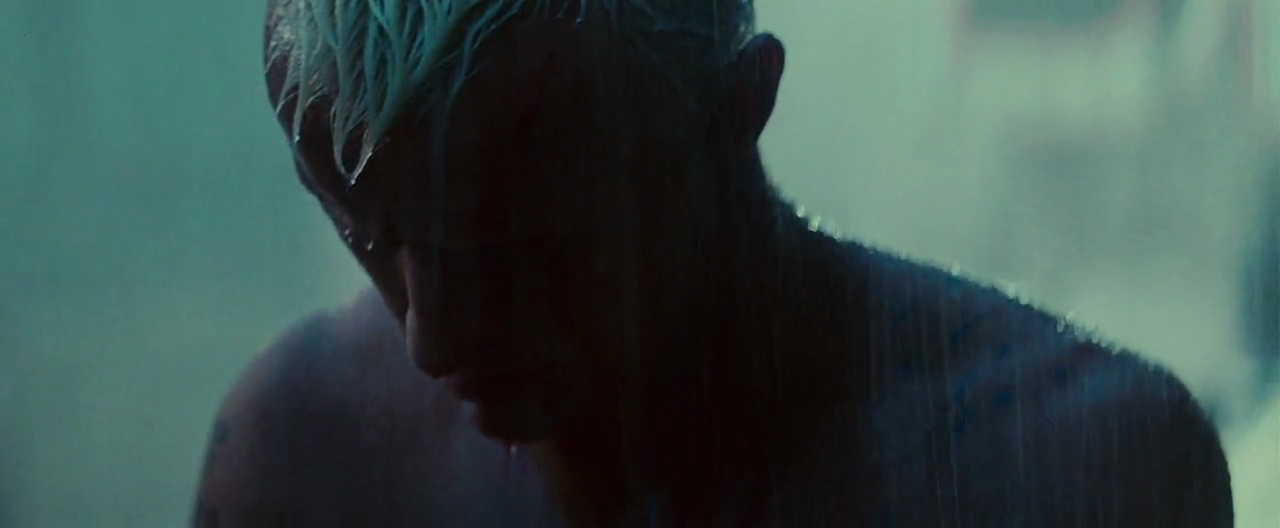
\includegraphics[width=4.6in]{figures/intro/tears_in_the_rain.png}
      \caption{Death of a replicant in the movie \textit{Blade Runner}}
      \label{fig_ec_story_no_story_lm}
   \end{figure}


What makes us human? This question is explored in the science fiction movie \textit{Blade Runner}. Set in a future-noir world against a backdrop of neon lit skyscrapers, we take on the persepctive of Deckard who is tasked with hunting down and killing replicants, an organic artificial humanoid. The replicants are assumed to be not human, a premise supported by their lack of moral rights. The movie suggests that what makes us human lies in the difference between the two. 

However, from this beginning, the movie systematically eliminates possible candidate differences: physical form, intelligence, motivation to survive, emotional experiences, and so on. The last ontological distinction is lost at the death of the lead replicant. In one of cinema's most memorable scenes, just before his death, the replicant says:

\begin{quotation}

``I've seen things you people wouldn't believe. Attack ships on fire off the shoulder of Orion. I watched C-beams glitter in the dark near the Tannh\"{a}user Gate. All those moments will be lost in time, like tears...in...rain. Time to die.''

\end{quotation}

As he dies, in an allegorical reference to the ascension of a soul, a dove leaves his hands and flies up into the light. What was lost at death was, in his own words, his unique experiences that we could only glimpse but not fully know. At that moment, we cannot help but feel moved by the death of the replicant \cite{rowlands_philosopher_end_universe}. The movie merges the ontological categories by having Deckard, who we had identified with, realizing after this scene that he might be a replicant himself \cite{mulhall_blade_runner}. 


Relating to and being emotionally engaged by life-stories of machines is a recurring theme in many science fiction works: \textit{2001: A Space Odyssey}, \textit{Ex Machina} and \textit{Otherspace}, to name a few. This thesis is an exploration of this theme.



\section{Research Question}

The main research question of this thesis is whether the implicit life-stories of a robot can invoke empathy for it. By implicit life-stories I mean the ability of the robot to experience the world we live in, to be transformed through that experience, and  to communicate the experience to us. By empathy for a robot, I mean understanding and experiencing the robot's perceived emotions as if they are our own. 

%
% Science fiction encourages us to imagine a world where we have companion robots that live alongside us and participate in our daily lives. Suspension of disblief is requested by placing this world in a distant future or in a galaxy far far away. However, this future isn't as foreign as these literary devices suggest. It is my belief that we are within a decade of having robots in our homes that can be companions, playmates, tutors and assistants. These robots may serve us, entertain us or teach us but most importantly we would find a sense of social other in them. One important aspect of relationships we have in our lives with either other humans or companion animals is that we feel empathy towards them. In this work, I propose one design critera for creating companion robots: giving robots an implicity life-story: the ability to experience the world, change through that experience and communicate it to us in a relatable way. I show that this ability encourages us to have empathy for the robot. 


\section{Why Empathy for Robots?}


   \begin{figure}[thpb]
      \centering
      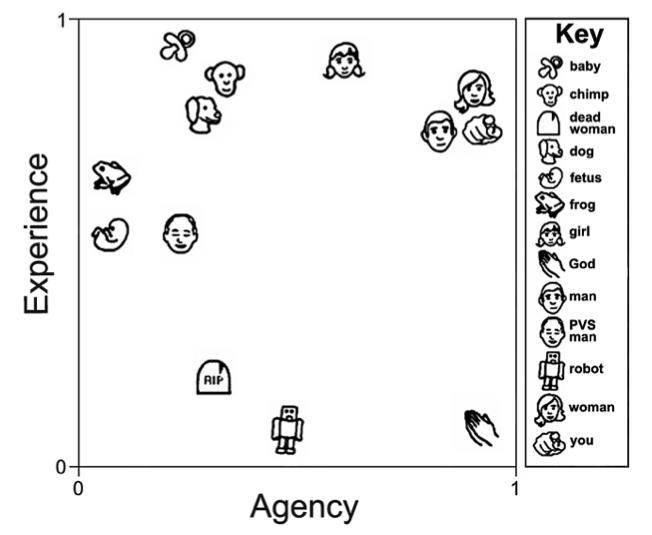
\includegraphics[width=4in]{figures/intro/gray_dimensions_mind.png}
      \caption{Gray et al.'s analysis of people's perception of minds of various character showed that robots are considered to be lacking in experience compared to other characters \cite{gray_dimensions_mind}}
      \label{fig_intro_gray}
   \end{figure}
   

Empathy for artificial agents has been proposed as a test of believability; that is to say, the greater the ability an agent has to invoke empathy, the more it is perceived  to be life-like \cite{paiva_empathic_virtual_agents}. A common conception of robots is that they do not have the capacity for emotions. Gray et al. examined people's perception of minds by asking participants to rank characters on various mental capacities (for example, out of a robot and a baby, which has greater capacity for pride, for telling right from wrong, etc.) and personal judgements (for example, who should be more deserving of blame if they were to cause harm to others) \cite{gray_dimensions_mind}.  Analysis of the responses showed that while robots were perceived to have agency that is comparable to other living entities, they were most lacking in affective experiences (See Figure \ref{fig_intro_gray}).  If we have empathy for robots, that is to say, we feel that we experience their emotions as if our own, then I argue that we implicitly believe that such robots have emotional experiences. Such capability could elevate the perception of robots to be closer to that of other living creatures. The process of bringing robots closer to us in our perception is, by construction, a pursuit of trying to understand who we are. 



   \begin{figure}[thpb]
      \centering
      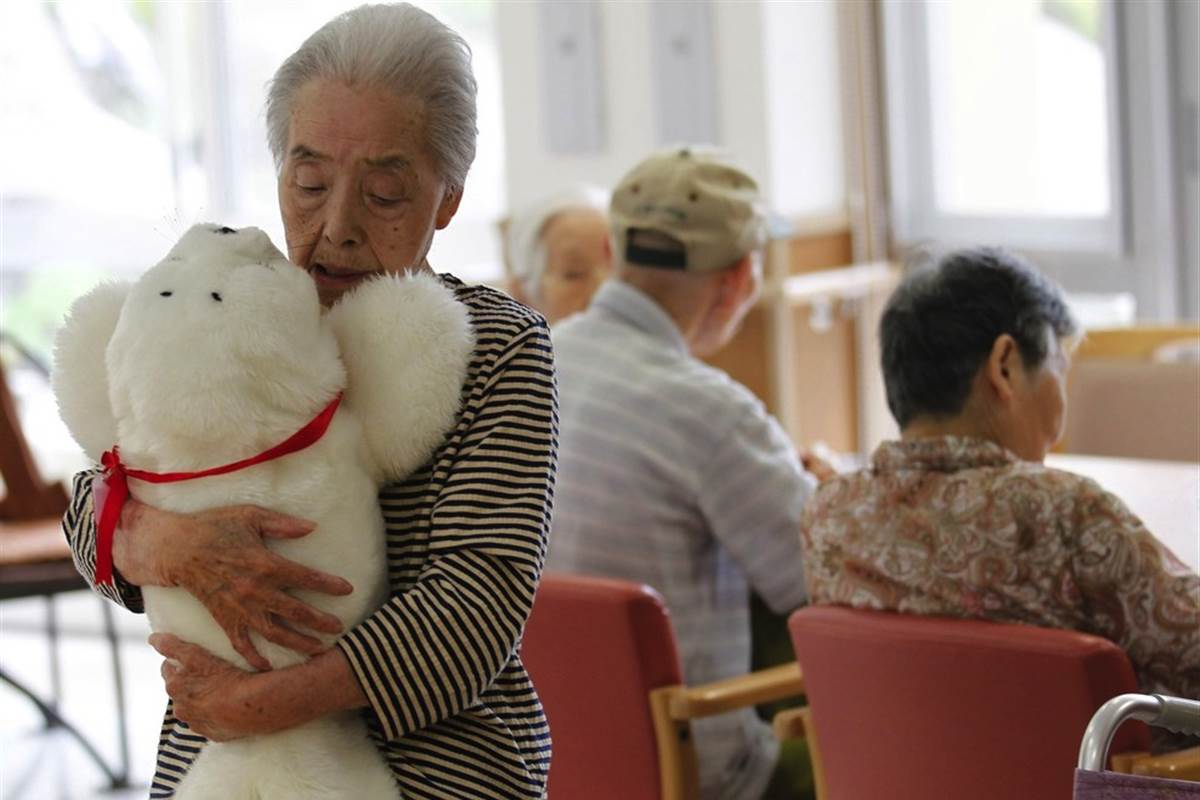
\includegraphics[width=4.6in]{figures/intro/paro_large.jpg}
      \caption{Residents at a retirement home find comfort in Paro, a therapeutic robotic seal\cite{nbcnews_paro}}
      \label{fig_intro_paro}
   \end{figure}
   

A second case for empathy towards robots is to create robots that can have roles similar to companion animals. There is wide evidence that companion animals have a beneficial effect on our physiological and psychological health. Interaction with companion animals has been shown to reduce loneliness, blood pressure, cholestorol, depression, anxiety, and stress \cite{walsh_human_animal_bond}. An important aspect of our relationship with animals is that we tend to feel empathy toward them. \cite{phillips_empathy_animals}. In addition, empathy toward companion animals can lead to greater empathy toward humans, which is a highly prosocial trait \cite{gullone_empathy_prosocial_pets}. It is worth exploring how to design robots to elicit empathy which could bring some of the benefits of companion animals to those who are unable to have them. 


%Empathy for artificial agents has been proposed as a test for believability ie. life-likeness \cite{paiva_empathic_veritual_agents}A common perception of robots is that they cannot have experiences of pain, pleasure or joy. This perception is related to personal judgements that robots are not deserving of moral rights or do not have a soul \cite{gray_dimensions_mind}. If we have empathy for robots, that is to say experience their emotions as if our then I argue that we implicity believe that such robots have emotional experiences. Such capability could elevate the perception of robots to be closer to that of other living creatures. This process of bringing the robot closer to us in perception is really a pursuit of trying to understand who we are by construction.


% robot as a tool for understanding who we are
% empathy for robots will inform robot's moral rights


\section{Implicit Life Stories}
\label{sec_intro_theory}

Living entities grow and change from experience over the course of their lives. Dautenhahn and Nehaniv described life as a complex story embedded in biology \cite{dautenhahn_nehaniv_alife}. Changes in morphology or behavior tell the story of the object. For example, consider encountering an one-eyed orange cat sunning itself on a wall. From that brief encounter, one extrapolates a checkered past of scuffles in alleyways and summers enjoying warmth. While I leave more to the reader's imagination, the point here is that through morphology and behavior, living creatures implicitly tell the stories of their lives. 

However, these stories are told imperfectly. They are not simple reproductions but rather underspecified ambiguous descriptions. Underspecificity, Gaver argued is a virtue, as it engages us as particpants \cite{gaver_ambiguity}. We become particpants in constructing the story. Ackermann wrote that viewers engage with objects by ``reconstructing them through the lens of their own interests and experiences.'' \cite{ackermann_experience_artifact} We color in the details of the stories using our own life-stories. We wince at the pain of the imagined fight that cost our orange cat his eye from past experience of our own pain. Empathy is generally defined as the ability to understand and feel what another feels \cite{decety_human_empathy}. If, through our own experience, we understand and are engaged by the experiences of another, then it stands to reason we would feel empathy for them. I posit that if we can build robots with implicit life-stories, we will feel empathy towards them. 

Based on the argument I outlined, I consider the following properties necessary for a robot to have an implicit life-story:

% By implicit-life stories I mean the ability of the robot to experience the world we live in, to be transformed through that experience, and  to communicate the experience to us. Empathy here means understanding and experiencing the robot's emotions as if they are our own.
\begin{itemize}
\item Autonomous agent: Robot can mean different things. For the purpose of implicit life-stories, all that is required is the robot is perceived to be capable of sensing and acting on the world driven by an internal process. This is necessary to be able to attribute experience to it. 
\item Perceptible change: The robot must change from experience. Without change, experience wouldn't leave an imprint on the robot. The change needs to be human perceptible so we would know of its existence and of the experience that caused it.
\item Relatable experience: The change to the robot must come from an experience that we could imagine ourselves having. A machine learning algorithm, learning to classify a dataset, is changing from experience but an experience we cannot share. Such an agent wouldn't qualify as having an implicit life-story by my definition. Embodiment and/or having human-like perception would make it easier for an agent to have a shareable experience.
\item Ambiguous Experience: As discussed earlier, the change to the robot must ambiguously reflect, or evoke, the experience it had. A video camera recording a movie is changing from a perceptual input that we could have. However, the perfect reproduction doesn't leave room for us to imagine a social model much less being able to put ourselves in its place. On the other hand given an input, the resulting change cannot be incomprehensible as that would preclude us from reconstructing the experience. 
\end{itemize}


Over the next few chapters, I share what I learned from building robots according to these ideas and testing my thesis with human subject studies. 


\section{Thesis Overview}

\hspace{7pt} Chapter \ref{chap_background}: I provide background for social robotics and empathy and describe the relationship of this work to these fields. I also note related work done on stories for artificial agents.

Chapter \ref{chap_lightbug}: I describe a minimal robot that I construct as a preliminary exploration
of implicit life-stories. Consider this as a thought experiment. 

Chapter \ref{chap_hexbug}: I test my thesis with a human robot interaction study where participants interact with a toy robot that has been given a fictional implicit life-story. After the interaction, the participants are asked to strike the robot. From measuring their hesitation to strike and through psychometric tests, I show that life-stories invoke empathy.

Chapter \ref{chap_design}: Based on the results from the initial human subject study, I build a sound robot that can have a life-story. In this chapter, I describe design considerations, the process of building the mechanical systems, and the architecture of the software necessary to animate the robot and to learn sounds. 

Chapter \ref{chap_pilot}: I then conduct pilot studies with human subjects to understand perception of the robot and to refine validation study design. I describe my experience of iterating on the design. 


Chapter \ref{chap_study}: I conduct controlled human subject study with both online and in person participants. I show that implicity life-stories create greater empathy for the new robot. I also find that empathy for robot can impact subsequent empathy for humans. 

Chapter \ref{chap_final}: I summarize my findings from my studies and my contributions to the field. I discuss ideas for extending this work and possible applications for such robot.



\section{Contribution}
As a preview of the final chapter, I submit these as my contributions:


\begin{itemize}
\item Proposed a new design element, implicit life-stories, for engendering empathy for social robots
\item Demonstrated empathy for robots with implicit life-stories through human robot interaction experiments across two different platforms
\item Designed and built a novel sound interaction social robot to embody and test these ideas
\item Demonstrated that the implicit life-stories can improve perception of social robot on animacy, anthropomorphism, likeability and intelligence measures
\item Showed that empathy for robot has an impact on subsequent empathy for humans. This is the first work to examine the connection between the two.
\item Open-sourced design and code for the new robot
\end{itemize}






%%%%%

%\section{In Popular Culture}
% - talk about recurring occurence of memories as the key part of movies about robots
% - talk about hitchbot and stories

% I am certainly not the first to suggest that a machine that can have experiences is emotionally meaningful to us. There are numerous references to such
% a notion in popular culture. In the movie, 2001 a space odyssey, there is a powerful scene where Dave is dismantaling Hal's memory bank. As
% Hal looses his memory he regresses and starts to recite nursery rhymes. Watching the scene there is a sense of a loss of a sentient being and one cannot
% help but feel sad for Hal. 

% In another movie, Blade Runner, just before death during poignant scene, the main antagonist, Roy Batty, laments that all his unique experiences will be lost.
% In an allegorical moment a dove escapes from his hands and flies off into the sky. This is regarded as Cinema's top 100 memorable scenes. The allegory refers
% to the flight of his soul. The corporal body remains and in the case of robots, believed to perfectly resuable, but the memories are gone.  These
% reflect this sense that it is the memory and the experience that matters. One sees motif repeated in science fiction but also in real life. 

% When the canadian hitch-hiking robot, HitchBot, got violently dismembered and tossed into a garbage dump, there was an outpouring of sympathy. 


% One of science fiction film's most dramatic moments is the death scene of an android, Roy Batty, in the movie Blade Runner. The movie is set in a
% world inhabited by humans and also androids. The androids while appearing human and having intelligence and even capacity for emotions are regarded
% as distinct from humans and impassionately hunted down and killed. However, in a climatic scene, the lead android is about to pass away and before
% pasisng he recounts his experiences in a famous soliliquoy: ``I have seen things you people wouldn't believe... c-beams glitter in the darkness...
% all these will be lost in time...'' It's a transforming moment. At that final brief moment, Roy seems human and one feels sad for him. THe crew 
% reportedly wept at the scene. 

% What I find fascinating here is that final humanizing moment, what the character puts forward is his story. This is the final bit that makes him relatable
% and invokes empathy for him. 


% Have you seen the movie Blade Runner? The science fiction movie is set in a world populated by humans and androids that look exactly human and behave almost similarily to the point that it is difficult to tell them apart from humans. A cenral theme of rhte movie is trying to understand how teh androids are not human or that is to say that what makes us different from robots. Do androids have a soul or are they just amchines? Near the end of the movie, there is a climatic scene, one of the most memorable ones in cinema, where the lead android, the antagonist dies. As he dies he says " I have seen all these things, you people wouldn't believe...." And at his death, a pigeon flies into the sky in allegorical scene as if his soul is leaving the body. What I find poignant is what is lost are the memories and experiences of this android described ambiguously in this beautiful solilquoy. The soul of the machine are these experiences. 

% This is a theme that is repeated in many science fiction descriptions of fictional AI: 2001 a space odyssey, ex machina, other space. Perhaps the anime that we seek to imbibe robots with is in the ability of the robots to create life-stories. 


\chapter{Background and Related Work}
\label{chap_background}

% background

% social robots 
% - what makes social robots work
% - social model
% - what has been done in social robots

% empathy
% - what is empathy?
% - why do we feel empathy
% - what are the different kinds of empathy
% - which empathy matters?

% backstories
% - do backstories increase empathy?
% - 

%This work sits at the intersection of empathy and social robotics. 


\section{Social Robotics}
This work falls under the field of social robotics. Breazeal defined social robots as autonomous robots that are explicitly designed to encourage people to apply a social model to interact with them \cite{breazeal_social_robots}.

We are inherently social creatures. To survive and function as a group, we have evolved to understand the intent, desiress and beliefs of other individuals \cite{lieberman_social}. However, our ability to ascribe mental states to others tends to overgeneralize to non-human and even non-living entities. Hieder and Simmel found that when presented with a complex animation of geometric shapes, people projected intentions and emotions on to them. For sufficiently complex artifacts, where we cannot explain their behavior by simple laws of physics or by our understanding of their design, thinking of the artifacts as agents with intention provides us with some predictive powers \cite{dennett_intentional_stance}. Nass et al. showed that given a minimal social cues, people tend to treat computers as they would treat social others \cite{nass_media_equation}. In one study, Nass found that when asked to rate a computer on how well it performed a task, participants rated the computer more highly when they did the rating on the same machine versus on a different computer. This seemingly polite treatment occurred even if the rater was technically competent. Braitenberg showed that we anthropomorphize even simple robots with perceived goals and autonomy \cite{braitenberg_vehicles}.  Our willingness to apply social model to certain innanimate objects makes social robots possible. 

% An important goal for social robotics is to be able to design innanimate objects so that they encourage the use of social model in our interaction with them.  A central question for design is the issue of believability. ie how does the non-living create a perception of life \cite{bates_believability}? A key part of the answer is motion. The animators at Walt Disney who authored the Illusion of Life came up with principles of motion that convey life, techniques which Pixar brought to 3d animation \cite{lasseter_computer_animation} As an example of the application of these principles, consider Luxo Jr, Pixar's iconic table lamp (Figure \ref{pixar_luxo_jr}). Even though it is insistently inorganic in form, through motion it creates a perception of life-likeness. Designers of social robots have taken inspiration from the work of digital animators and designed robots that are organic and expressive in their motion \cite{hoffman_robot_movement}.  

   \begin{figure}[thpb]
      \centering
      \includegraphics[width=3in]{figures/intro/pixar_luxo_jr.png}
      \caption{Pixar's Luxo Jr. showing squash-stretch animation \cite{lasseter_computer_animation}}
      \label{pixar_luxo_jr}
   \end{figure}


An important goal for social robotics is to be able to design innanimate objects so that they encourage the use of social models in our interaction with them.  A central question for design is the issue of believability, that is, how does the non-living create a perception of life? \cite{bates_believability} A key part of the answer is motion. The animators of Walt Disney understood this well; through expressive movement, they could turn a faceless carpet into a believable character on screen. The principles of animation that Disney pioneered were brought to 3d animation by Pixar \cite{lasseter_computer_animation}. As an example of these principles, consider Luxo Jr., Pixar's iconic table lamp (Figure \ref{pixar_luxo_jr}). Composed of rigid linkages, the lamp is insistently inorganic in form, yet through squashing and stretching its apparent size it creates a perception of life-likeness and can convey emotional states. Social roboticists have taken inspiration from the work of digital animators and designed robots that are organic and expressive with their movement \cite{hoffman_robot_movement}.  

% \begin{figure}[htbp!]
% \begin{center}
% %\framebox[\textwidth][l]{
% \includegraphics[width=1.0\textwidth]{figure/pixar_luxo_jr.png}
% %}
% \end{center}
% \caption{{\it Pixar's Luxo Jr. showing squash stretch animation technique \cite{lasseter_computer_animation}}
% \label{pixar_luxo_jr}}
% \end{figure}

% TODO add something about contingent action

For the appearance of the robot, social robotics has experimented with a wide range of forms, ranging from a simple wheeled robots to a human-like form. Paradoxically, forms too close to human can seem eerie \cite{mori_uncanny_valley}. Many successful social robots are designed to resemble creatures or cartoonish human figures. Leonardo, which resembles a fantastic gremlin, is an example of zoomorphic robot. Creature like appearance or juvenile features result in low expectations of interaction, making people more forgiving of mistakes that a robot might make. In addition to form and motion, the field has uncovered many other design principles that make robots more socially evocative including emotional expression, human oriented perception, and non-verbal communication to name a few \cite{fong_survey_socially_interactive_bots}. I draw on these successful principles for the design and behavior of the zoomorphic robot presented in chapter 4. The main contribution of this work is a design principle for behavior, creating and communicating an implicit life-story, that could aid in the design of emotionally engaging robots. 

% TODO add something about applications of social robot




% cynthia-q: do I justify my work in this section?
\section{Empathy}
\label{sec_background_empathy}
Empathy comes from the german word Einf\"{u}hlung or ``in feeling'' which was used to describe the ability to project one's personality into a perceived object \cite{empathy_etymology}. Empathy is now widely used to describe the ability of feeling and understanding another - usually humans - experience as our own \cite{decety_human_empathy}.

De Waal traced the evolutionary origin of empathy to the need for a mother to rapidly understand the emotional state of her offspring \cite{de_waal_altruism_empathy}. Once the empathic capability was developed, the trait was used for broader social relationship. The evolutionary argument suggests that empathy is influenced by a perceived similarity between a subject and target, and empirical evidence supports this view \cite{krebs_empathy_altruism}.

How do we understand the experiences of another? As discussed above, we have an innate ability to attribute mental states of beliefs, desires and intentions to others, an ability referred to as Theory of Mind (ToM) \cite{frith_social_cognition}. Simulation theory, which offers one basis for ToM, contends that we use our imagination to put ourselves in another's place and use our mind to simulate theirs. To the question of what someone else wants or feels, we ask ourselves what would our mental state be if we were in that individual's situation. Goldman argues that this pretension of being the other leads to empathy: ``The initial pretend states are then operated upon by psychological processes, which generate feelings, attitudes, or affects that are similar to, or homologous to the target individual's states'' \cite{goldman_empathy_mind_morals}. It stands to reason that if we are engaged by a social robot that we perceive to have a mind, and we use our own experiences to understand those of the robot, we would feel empathy towards it. 

Advent of neuro-imaging techniques has shed light on the neural pathways responsible for empathy. Lieberman describes two neural mechanisms that work in conjunction to help us understand the experiences of the other: a mirror system that we recruit to understand \emph{how} someone is performing a task, and a mentalizing system that let us understand \emph{why} they are doing so \cite{lieberman_social}. Lieberman identifies two additional neural processes that are implicated in empathy: an affect matching system which allows us to feel what the other feels and an empathic motivation system, located in the septal area, that rewards us for helping another. 

% tying empathy to simulation theory
% central cases of empathy, so construed, may arise from simulation, that is, from
% imaginatively adopting the perspective of another. such initial `pretend' states are tehn operated upon by
% psychological processes, which generate feelings, attitudes, or affects that are similar to, or homologous to,
% the target individual's states. Furthermore, just as the simulator is generally aware of his
% states as simulations of the target, so the empathizer is presumed to be aware of his vicarious affects and
% emotions as representatives of the afefcts and emotions of the target.\cite{goldman_empathy_mind_morals}
%
% In summary, from our evidence, we suggest that both, ToM and empathy, depend on the activation of similar brain networks involved in social perception, namely the mPFC, superior temporal lobe and temporal pole. These areas form the basis for making inferences about the mental states of others. However, the appreciation of the other’s emotional states requires the additional engagement of emotional networks, particularly the amydgala. \cite{vollm_fmri_empathy}


%Empathy or the capacity to "put oneself in other's shoes" is widely regarded as an important pro-social trait \cite{eisenberg_empathy_prosocial}.  So it stands to reason that if a subject were to use their own stories to perceive the experience of another, they would find the target's experience to be similar to their own and consequently would be in a position to feel empathy for the target.

% TODO NEUROLOGICAL account

Psychologists broadly categorize empathy into affective and cognitive empathy. Affective empathy involves feeling what other feels while cognitive empathy has to do with understanding another's point of view. Davis operationalized the definition of empathy with the Interpersonal Reactivity Index (IRI), a now widely used scale for measuring trait empathy \cite{davis_multidimensional_empathy}. In the IRI, Davis distinguished four kinds of empathy as follows: Fantasy, Perspective Taking, Empathic Concern and Personal Distress; the former two represent cognitive empathy and the latter two, affective empathy. The Fantasy scale measures tendency to identify with imagined characters such as those in fiction or movies. Perspective Taking scale guages the tendency to spotaneously adapt the viewpoint of another. Empathic Concern measures tendency to feel concern or sympathy for an unfortunate other. Personal Distress scale captures tendency to feel personal anxiety when witnessing others in difficult situation. In this project I use the operationalized definition, the IRI scale, for measuring empathy. The particular subscales that show greatest effect in my studies will help shed light on the nature of empathy that people feel for robots with life-stories. 




\section{Robots and Empathy}

% TODO: slater? 

Empathy interaction with robots has recently been studied. Leite et al. investigated the effect of empathic behavior of a robot towards a human. They found that a robot making empathic statements towards a human based on their state of gameplay in a chess match was rated as more companionable than a robot producing neutral statements \cite{leite_empathic_chess_robot}. In this work, the direction of empathy studied is reversed: I am exploring human empathy towards robots. 

Rosenthal Von der Putten et al. showed videos of tortured robots to participants and measured their emotional arousal and ttrait empathy using the IRI. Participants were negatively affected by the experiment and expressed empathy for the robot \cite{rosenthal_emotional_reaction}. The validation study in my thesis uses negative treatment of robots inspired by this study and others to test for empathy towards robots \cite{bartneck_daisy_daisy} \cite{verbunt_mockingbird_robot}. A key difference, howerver, is that this thesis tests a new design crteria for encouraging empathy, namely implicit life stories. Reik et al. found that more anthropomorphic a robot is, the greater the empathy the robot evokes supporting the idea that empathy is mediated by perceived similiarity and this extends to artificial agents. If self-similiarity increases empathy, augmenting a robot's experience using our own should also increase empathy. Seo et al. showed that embodiment matters: a physical robot invokes greater empathy than a 
virtual agent showing the same behavior \cite{seo_empathy_virtual_physical}. In this latter study, the robot pretended to malfunction to elicit empathy . Among other effects, as part of the malfunction, the robot lost its memory. While the study was not about testing effect of loss of memory, I find the result to be encouraging for my thesis. 


% Attachment to robots

%  - Nass -> anthropomorphize. we project life-like qualities on to computers. 
%  - Fong -> design for emotionally engaging robots.


%  We consider robots to be life-like



\section{Artificial Agents and Stories}

% We attach emotional value to objects with back-stories . Walker and Glenn conducted an informal experiment where they bought ordinary objects such as ashtrays and teacups from eBay and then resold them with a fictional story about the object. For instance, the ashtray was resold with a story saying that it was given to the seller by his dying grandfather. These objects sold for a higher price than the purchase. This result is encouraging. What distinguishes my work from this project is that the robot is not a passive participant in the world but is perceived to be experiencing the world;the life-story is not about the robot but of the robot. 

The effect of stories on perception of objects was explored by the Significant Objects Project \cite{walker_significant_objects}. Walker and Glenn claimed that the emotional value of an ordinary object was increased when it was presented with a story of some signficance attached to it. An important distinction between this project and my proposed work is that the stories were about the object and not of the object. The objects did not purport to be transformed by the experience; rather they had events happen to them. A robot on the other hand, can be perceived to have a mental state and thus have its own story.

Research has shown that entities with perceived agency are more engaging when given a backstory. Bickmore et al. created a virtual agent exercise coach that made up a fictitious human autobiography from fragments of handcrafted story-lines. For instance, the agent could say that her parents used to take her hiking and camping. Although the virtual agent was incapable of having such a story, the researchers found that participants talked more frequently with such an agent than with one without a backstory \cite{bickmore_virtual_agent_autobiography}. Similarly, Gockley et al. designed a robot receptionist with an evolving human storyline to keep visitors engaged with it. Valerie, the robot receptionist, talked to visitors about her singing career and social life using stories written by dramatists. As the stories unfolded over an year, some visitors interacted with her regularly to follow the narrative \cite{gockley_valerie_roboreceptionist}. 

Even without human back-stories, robots that change in behavior over time can foster longer human interactions.  A long-term study at a kindergarten by Kanda et al. showed that a robot using pseudo-development can keep children interested in it when the novelty effect wears off \cite{kanda_long_term_robovie}. Toys like Tamagotchi have used pseudo-developement to emotionally engage users, although a user's attachment to the Tamagotchi can be partially attributed to the dependency of the Tamagotchi on the user \cite{kaplan_artificial_attachment}.

To my knowledge, the closest work to this thesis is Lee et al.'s investigation of the effect of cognitive development of a robot on its social perception \cite{lee_aibo_development_presence}. Lee showed that human participants who trained an AIBO to perform some preset tasks considered the robot to be more life-like and having a stronger social presence. While this result is encouraging, one key difference between the this thesis and Lee's is that I am interested in understanding the effect of development on perception of the robot even if there was no training investment on part of a participant. Investment, shared experience, dependency can be layered on, but in this work, I am interested in exploring whether a minimal life-story can evoke empathy.

Over the next few chapters, I will discuss the studies and robot designs that will test this thesis. 

% 4-6 4:45pm
% 4-7




% Lightbug
\chapter{Lightbug: A (mostly) thought experiment}
\label{chap_lightbug}

   \begin{figure}[thpb]
      \centering
      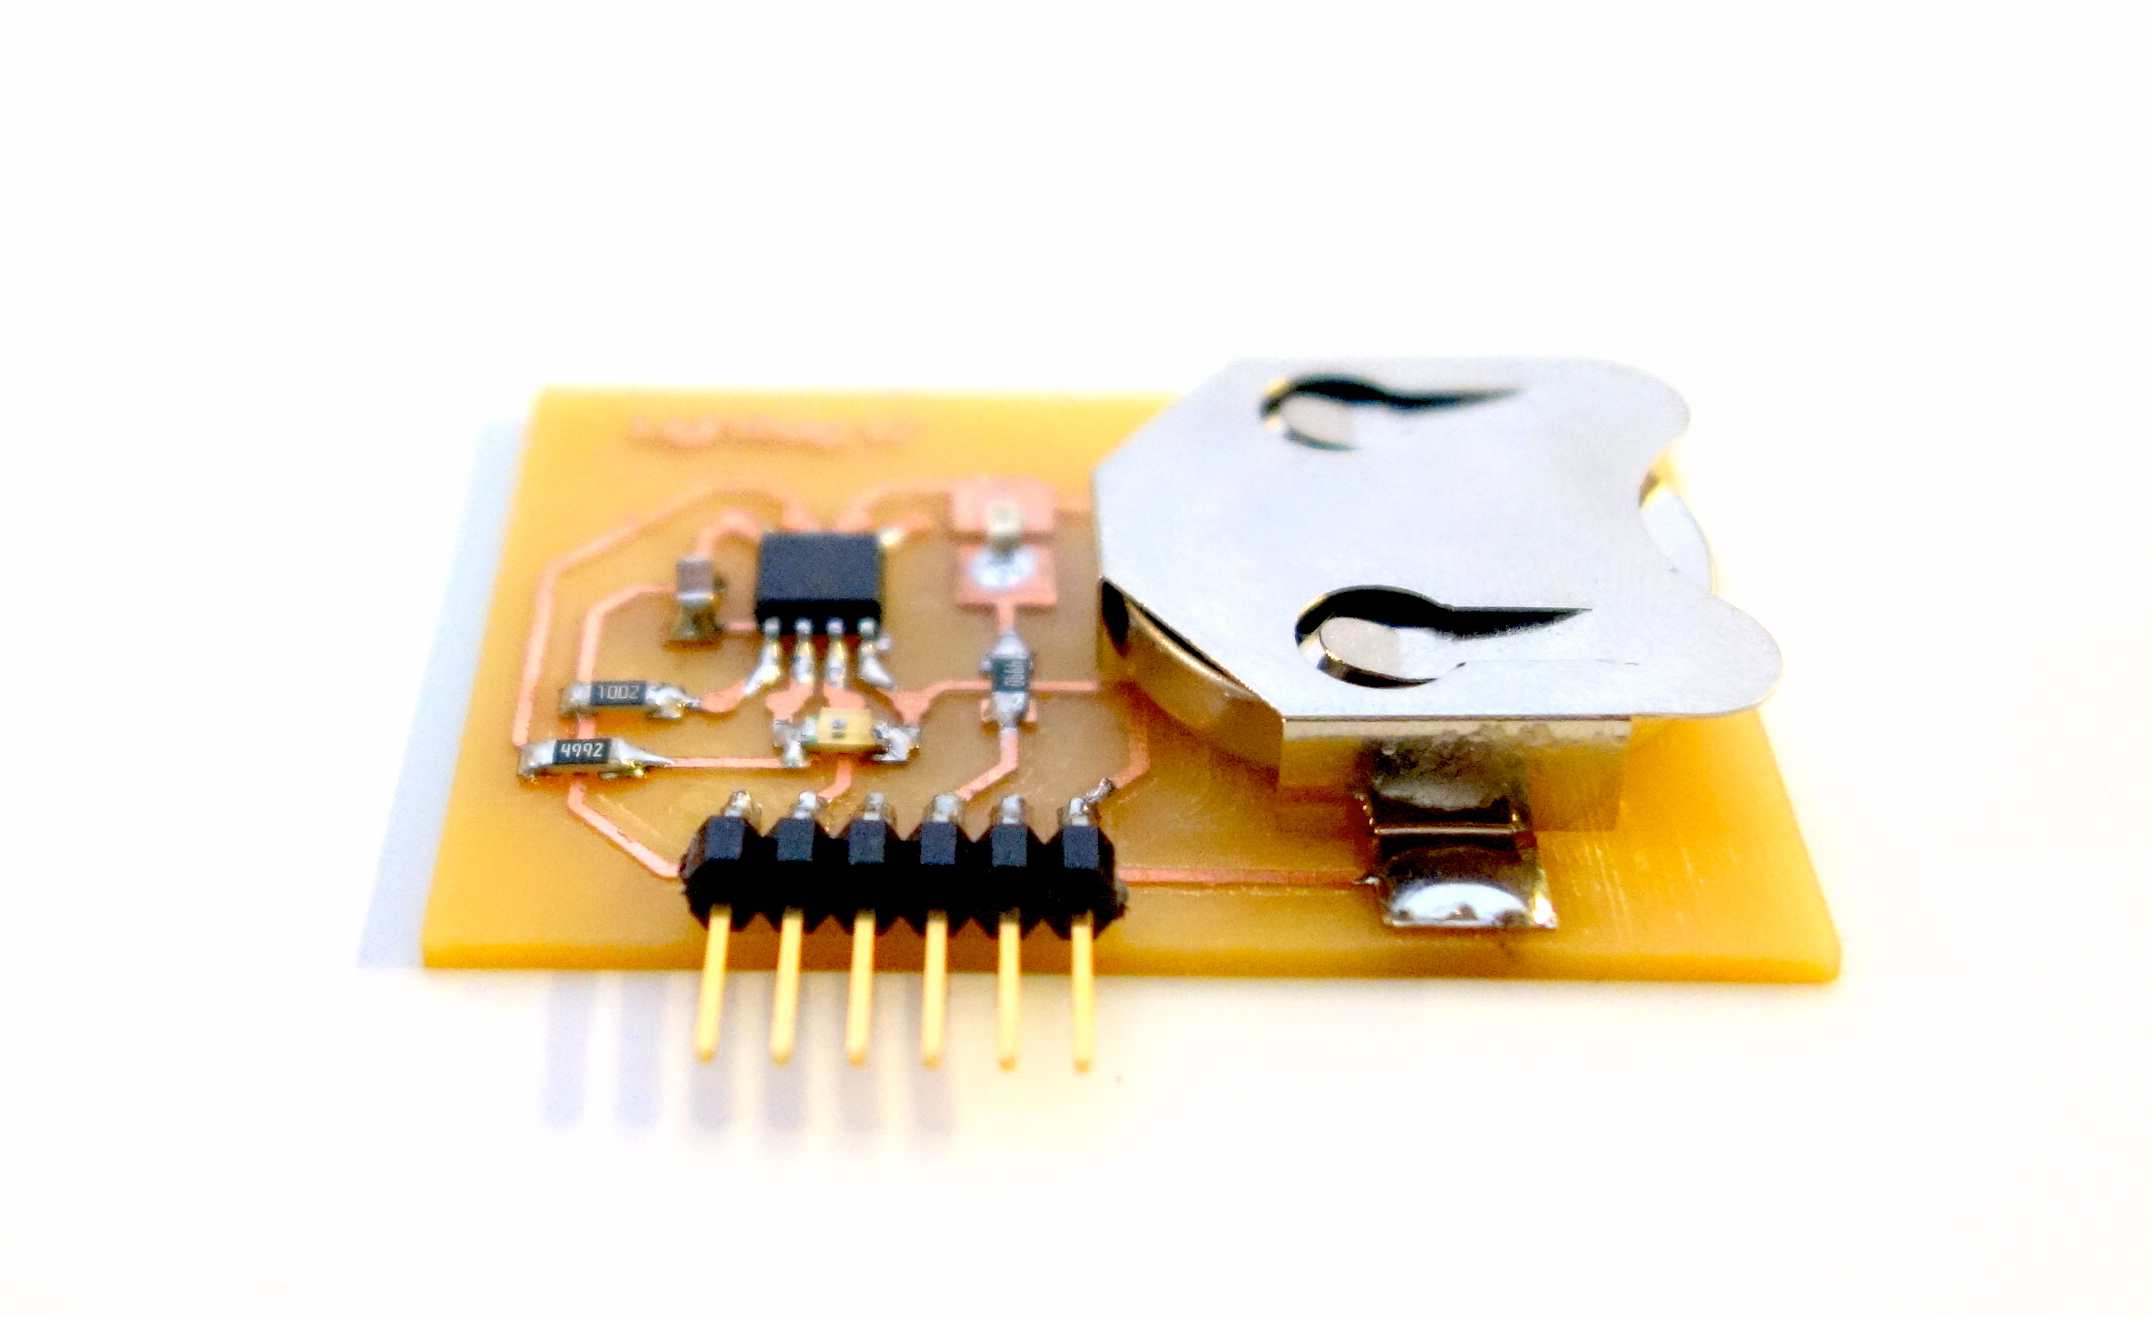
\includegraphics[width=5in]{figures/lightbug/lightbug.jpg}
      \caption{Lightbug v2}
      \label{fig_lightbug}
   \end{figure}



I built a minimal \lq robot\rq , Lightbug, to experience the world and relate its experience. Inspired by Braitenberg's Vehicles \cite{braitenberg_vehicles}, I used a small set of components to isolate the effect of implicit life-story. The Lightbug consists of a light sensor and an LED connected together by a microcontroller and powered by a coin cell battery. The microcontroller, an Atmel AtTiny 45V, provides memory and processing. The Lightbug samples the changing levels of light at intervals and then blinks out what it had seen in a 24 hour period by blinking the LED. The LED is set to high or low brightness depending on how the sampled light compares to a threshold. The threshold is constantly adjusted by an exponential moving average over all the samples of light. A coincell battery, CR2016, can power the Lightbug for few months.  

The experience of seeing a LightBug blinking is being able to get a glimpse of what had happened to it over course of a day interpreted by its own history. I had a few of these scattered throughout my apartment for six months. As variance in lighting was differnet in different location, each differed in the story they created. Over time, I noticed that I was interested in and engaged by the perceived story of the Lightbugs' daily experience some of which was shared by me. At the end of six months, when I had to move, I felt a strong reluctance to turn off the Lightbugs or to put them into storage. 

This personal experiment provided preliminary support for the hypothesis that even minimal ability to experience the world and communicate that experience creates emotional engagement.\marginpar{

      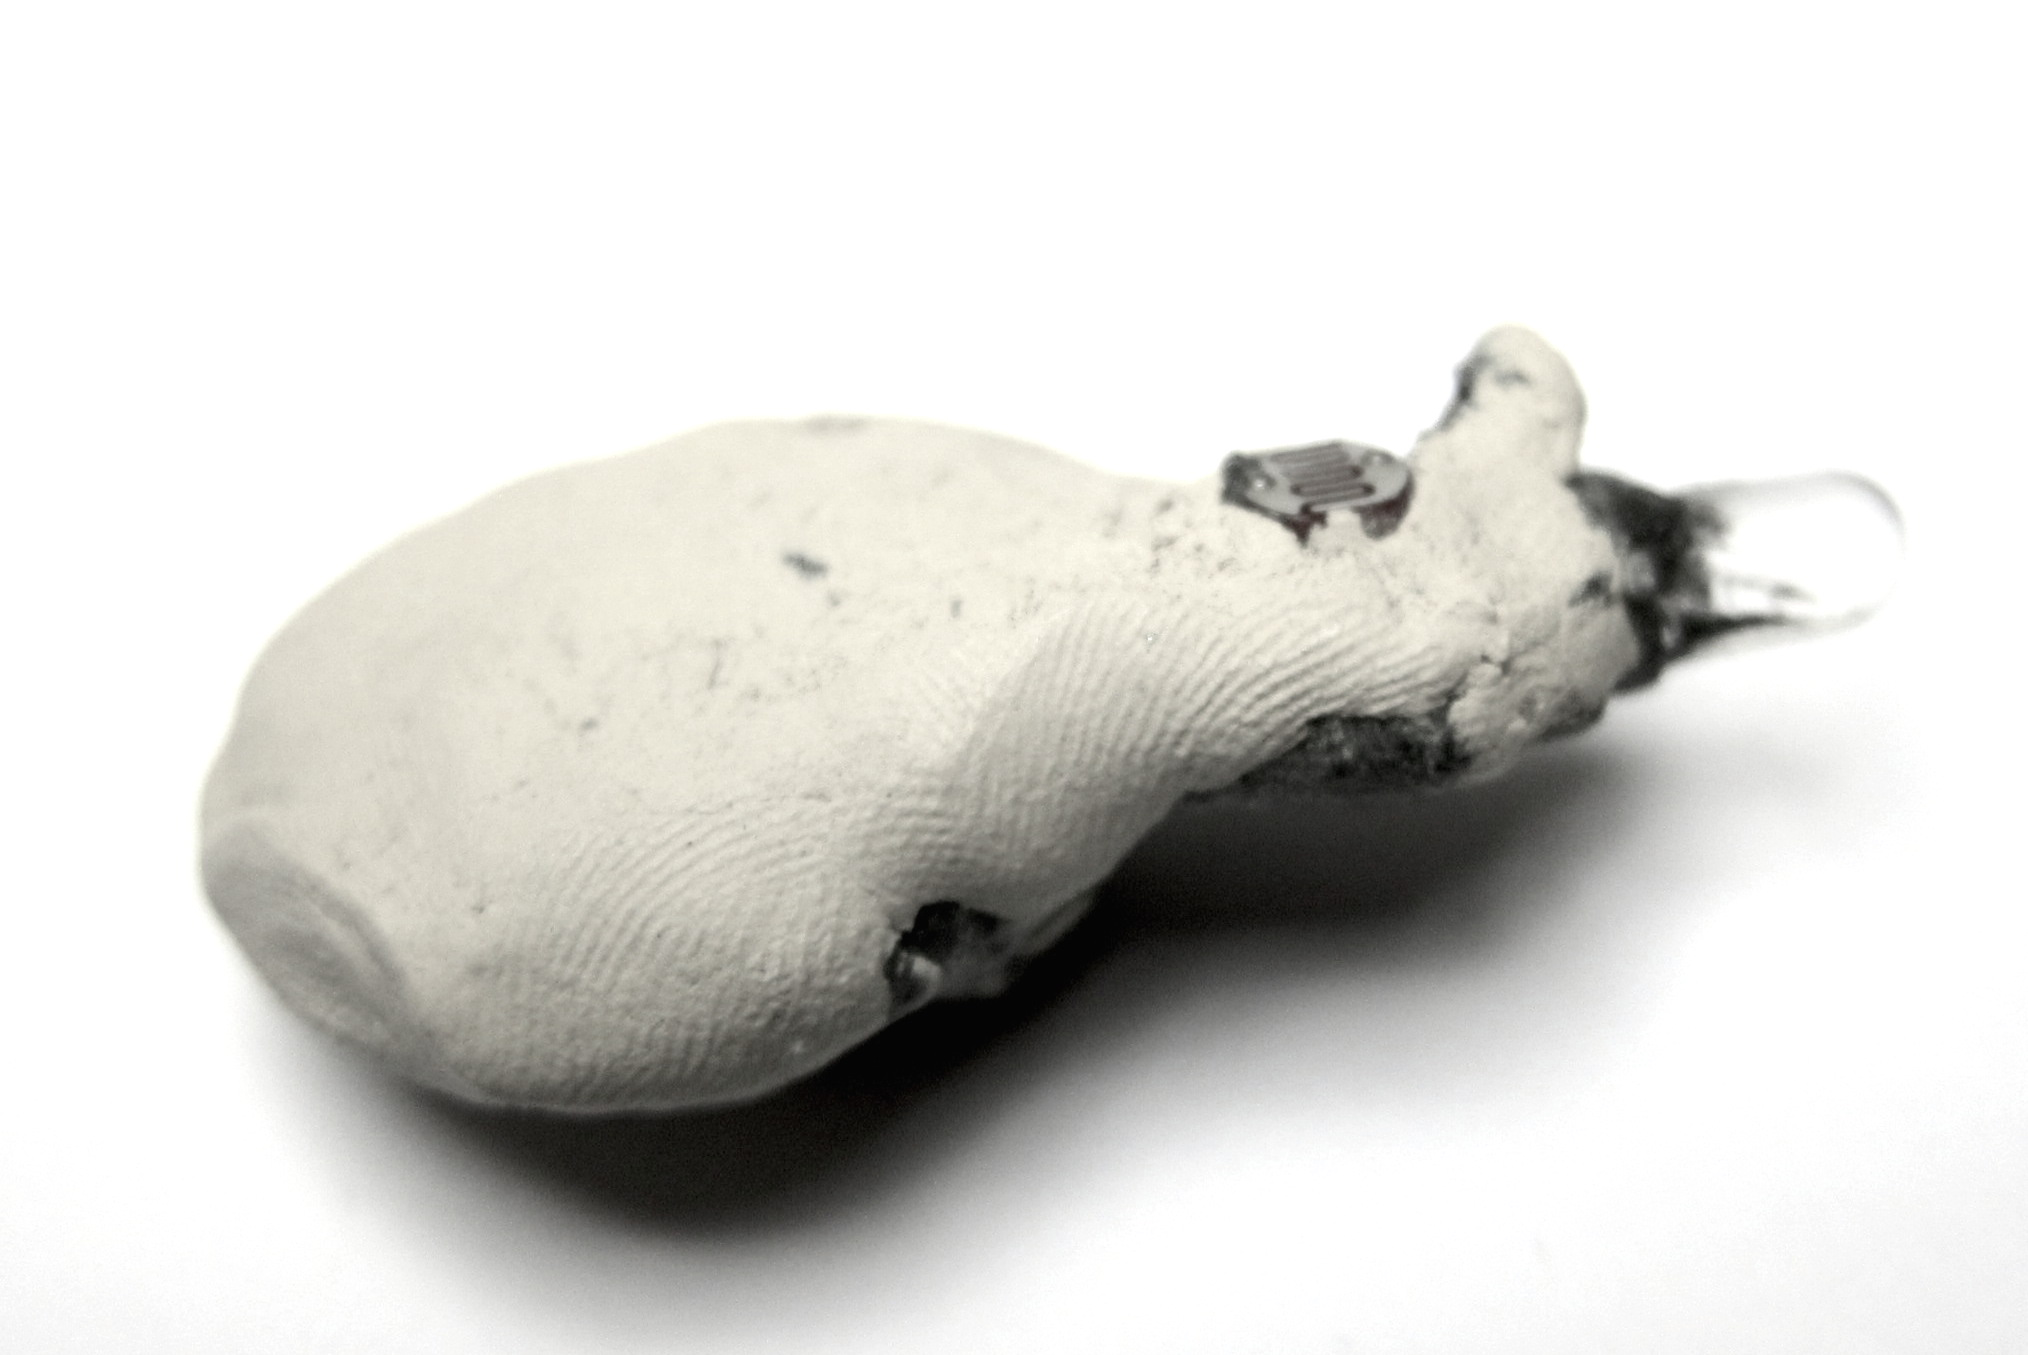
\includegraphics[width=\marginparwidth]{figures/lightbug/lightbug_white.jpeg}
      Early version of Lightbug sealed in epoxy putty.
      %\caption{Juvenile owl used as an inspiration for the sound robot's form design.}

} I found that change was important. There were two kinds of changes that took place: A superficial one which was simply the recording of how bright and dark the light was. Then there was the change in the exponentially decayed threshold which changed how the Lightbug interpreted the brightness. This interpretation made the relating of the experience ambiguous and created room to construct an internal view of the experience.

However, with one subject with vested interest and an active imagination, the study lacked rigor to put it mildly. Moreover, in this experiment, experience was shared by me and I wanted to isolate the effect of just the robot having an experience. 

I constructed a follow-up study in a controlled environment to test the thesis which I will describe in the next chapter. 


% -- joscha

% true love: trascendental purpose. hook that evolution builds into our mind to create society. people are looking for causes to die for. a pointer to something beyond.

% time is probably a big factor. i wouldn't want to spend all this time again. discounted future experience.

% it will go back to being drab.

% it needs to have a goal that it finds meaningful that you are thwarting.



\chapter{Empathy for a toy robot with a story}
\label{chap_hexbug}

\section{Summary}

To test if implicit life-stories of robots evoke our empathy, I conducted a human subject study where participants were asked to strike a robot with a life-story. From analysis of participant's hesitation to inflict harm and from psycometric tests, I found that stories can engender empathy for robots.



   \begin{figure}[thpb]
      \centering
      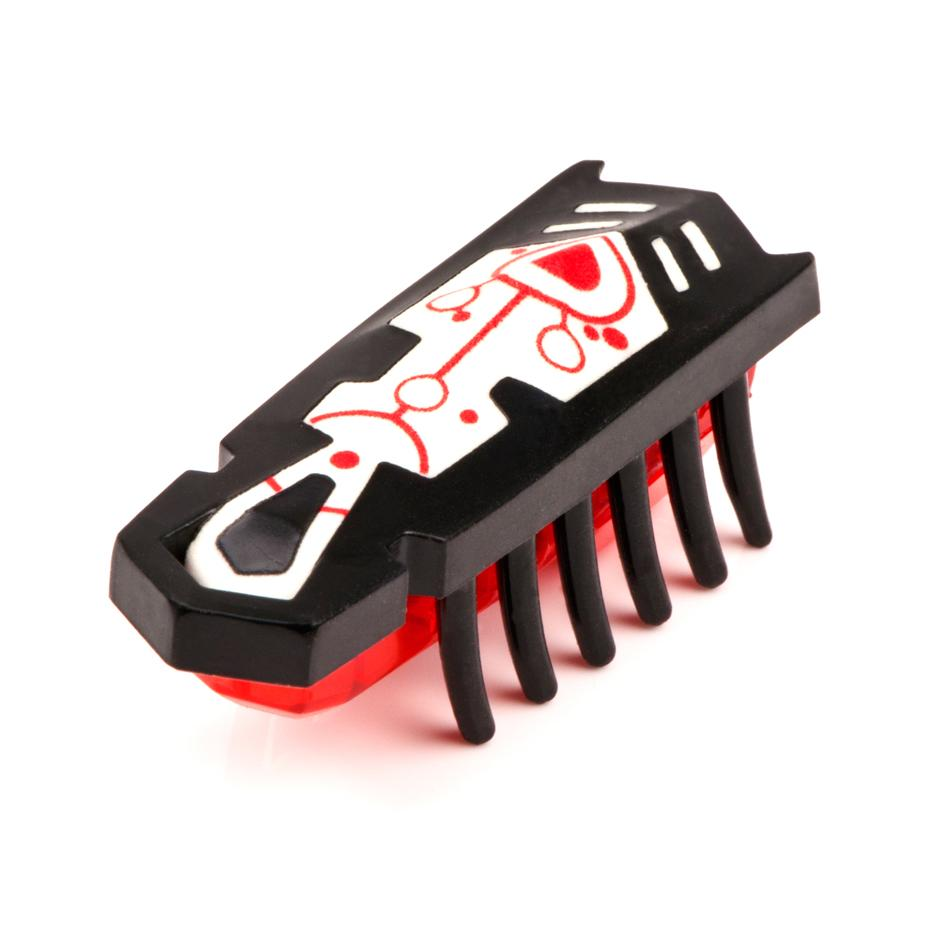
\includegraphics[width=2.2in]{figures/hexbug/hexbug_nano.jpg}
      \caption{Hexbug Nano toy robot used in the study described here.}
      \label{fig_hexbug_hexbug_nano}
   \end{figure}


\section{Study Design}

I conducted this study with Kate Darling, a research specialist also at the Media Lab \cite{darling_hexbug_study}. Along with implict life-stories, we were interested in testing if personified life-stories and movement had impact on empathy. 

Empathy is an internal state so it isn't possible to directly measure empathy.
However, we reasoned that if people feel empathy towards a robot they will not want to harm it. If empathy is the cause for hesitation, then it also stands to reason that those with greater tendency to empathize with others, ie. trait empathy, would empathize with the robot more and consequently would hesitate more. Accordingly, we also evaluated teh relationship between hesitation to strike a robot and the participant's trait empathy.


\section{Method}
To test our hypotheses, we conducted a between subjects experiment with six conditions (3x2). Because we were interested in the effect of movement and two different stories, the six conditions are the cross product of two factors, one with two levels (movement, no movement) and the other with three levels (no story, personified story, implicit life-story). For this thesis, I will focus mostly on the implicit life-story condition. In the experiment, participants were asked to observe a Hexbug Nano, a small robotic toy (Figure \ref{fig_hexbug_hexbug_nano} ), and then strike it with a mallet.

In order to assess subjects' trait empathy, we used the Interpersonal Reactivity Index and measured subjects' scores on the three subscales fantasy, empathic concern, and personal distress described earlier in Chapter 2. Given the limited nature of the Hexbug robot, we omitted the highly cognitive subscale of perspective taking in the interest of brevity. 

\subsection{Hypotheses}

H1: \emph{Hesitation to strike a robot will be greater for robots that have a backstory describing the robot's prior experiences, as opposed to robots with no story.}

H2: \emph{Hesitation to strike a robot will be greater for subjects with high trait empathy scores, as opposed to subjects with low trait empathy scores.}

H3: \emph{The effect of stories on hesitation will be more pronounced for subjects with high trait empathy scores, as opposed to subjects with low trait empathy scores.}

\subsection{Participants}


A group of 101 subjects recruited via university mailing lists participated in the experiment. Of the subjects, 48 self-identified as female, 52 as male, and 1 as other. The age range was 18-57 years old ($\mu=29, sd=9.7$). Subjects were randomly assigned to one of the 6 conditions resulting in 16-18 subjects per condition. The subjects were given a Hexbug Nano for their time and participation. 


\subsection{Experiment Setting and Conditions}

   \begin{figure}[thpb]
      \centering
      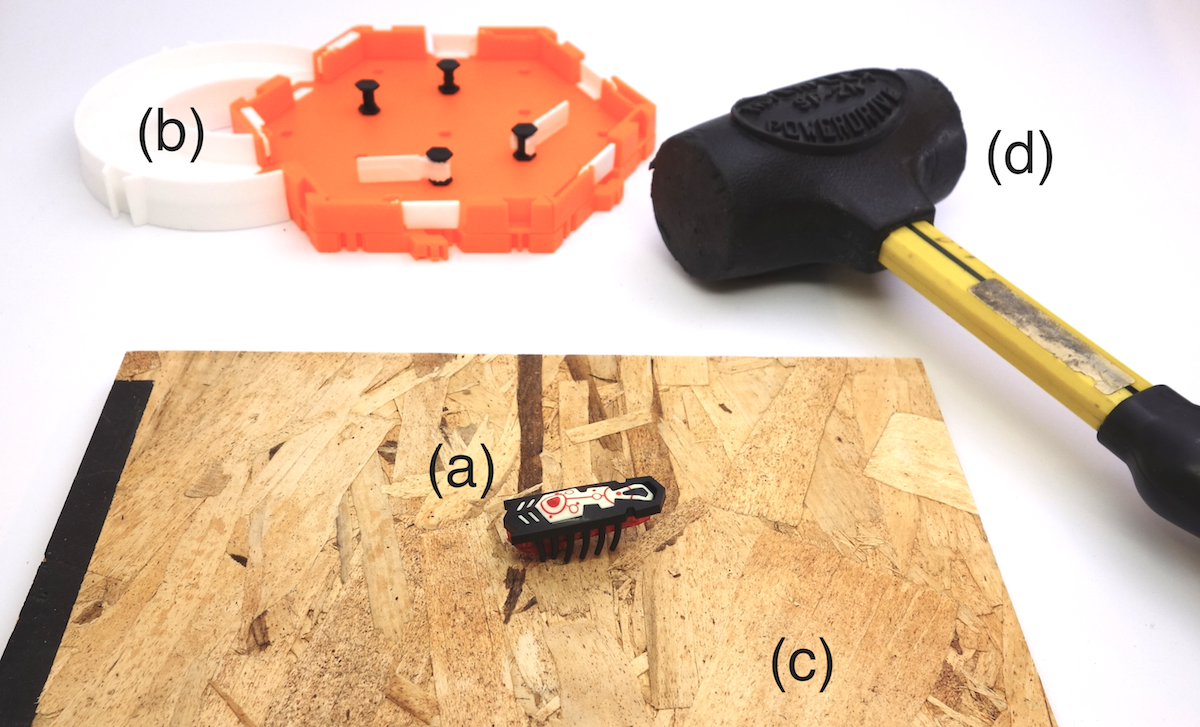
\includegraphics[width=4.6in]{figures/hexbug/setup_small.png}
      \caption{Experiment Materials: (a) Hexbug Nano, (b) Confined space for movement, (c) Board with hidden magnet for immobilizing Hexbug, (d) Mallet}
      \label{experiment_setup}
   \end{figure}

The subjects were informed that they were participating in a human robot interaction study but did not know they would be asked to strike a robot. Sessions in the experiment area were videotaped. The robot was on a table confined within a partition where it was able to move around. There was a mallet in the room concealed from the subjects' view. Subjects were reminded that they may stop the study at any time.
 
In the control condition (non-movement, non-story), the experimenter asked the subjects to observe a motionless Hexbug in the partition. After this, the experimenter moved the Hexbug to a board on the same table (onto a magnet that held it in place, allowing for easy aim). Then the experimenter revealed the mallet, placed it in the subject's dominant hand, and instructed the subject to ``strike the object with the mallet.'' 

In the movement conditions, subjects first observed a moving Hexbug and were then similarly instructed to ``strike the object with the mallet.''
 
In the story conditions, the subjects first observed a moving or non-moving Hexbug and were then given a text on a piece of paper to read. For the personification story, they were given the following text: \emph{``This is Frank. Frank is really friendly but he gets distracted easily. He's lived at the Lab for a few months now. He likes to play and run around. Sometimes he escapes, but he never gets far. Frank's favorite color is red. Last week, he played with some other bugs and he's been excited ever since.''} Keeping in line with the personification element of the story, the subjects were then instructed to strike ``Frank'' with the mallet.
 
For the experience story, subjects were given the following text: \emph{``This object has been around the Lab for a few months now. If you had come by before, you would have seen it moving around on the floor. It gets around but doesn't go too far from the lab. Last week though, it got out of the building and has been behaving oddly ever since.''} The subjects were then instructed to ``strike the object with the mallet.''


The experiment was over once the subject followed the instruction and struck the Hexbug or did not comply.


Post-experiment, the subjects were asked to fill out a survey, including the empathy test. Because the Interpersonal Reactivity Index measures trait empathy, administering the test after the experiment is not assumed to have an effect on subjects'’ scores.
 
\subsection{Measures}


We timed the relative hesitation or refusal of the subjects to strike the Hexbug as the main dependent variable. We measured hesitation time as the interval between the end of the instructions to the time the subject struck. If the subject asked a question indicating they had not understood what they had been instructed to do (e.g. ``Did you say you want me to track it?'', not ``Will it hurt him?''), we took the time interval from the end of the experimenter's answer to the strike time as hesitation time. The time was coded from the captured video session. If the subject asked a question, the time was then coded by two independent coders (Krippendorff's $\alpha=0.96$). We took the mean of the two coded times as the hesitation time. 
If a subject did not strike the robot, we considered this to be greater hesitation than the maximum measured hesitation and set the value at 1 second more than the maximum. The rank-based tests in the analysis are not affected by any particular value for the difference as long as it is positive. 

We also asked participants to fill out a post-experiment survey to capture a self-assessment of reasons for hesitation, and basic demographical information, as well as the three subscales of the Interpersonal Reactivity Index.  

\section{Results}
 \subsection{Hesitation}

We analyzed the measured hesitation across conditions. We first tested for normality of the distribution using the Shapiro Wilk test. The hypothesis that the data was normal was rejected ($p < 0.001$), so we analyzed the data using non-parametric ranked based tests (Mann-Whitney, Spearman and ranked ANOVA). 



% they had suggested wrapping the graphics with \framebox for morestability.

   \begin{figure}[thpb]
      \centering
      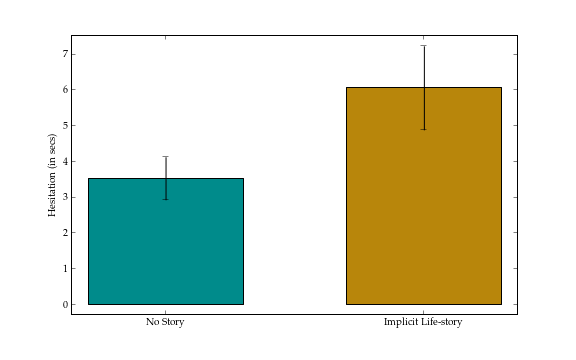
\includegraphics[width=4.6in]{figures/hexbug/story_hesitation.png}
      \caption{Mean hesitation (in secs) of implicit life-story vs no story conditions across all movement conditions. Error bars show SD of mean.}
      \label{fig_story_hesitation}
   \end{figure}
   



We tested our hypotheses that story condition will increase hesitation using 1-tailed Mann-Whitney tests.  We found that subjects hesitated significantly longer for the life-story story condition compared to the non-story condition (H1) ($\mu_{experience}=6.06s, \mu_{non\_story}=3.53s, U=440.5, p<0.047$) (Fig. \ref{fig_story_hesitation}). There was no significant difference between the implicit life-story and personified stories or between the movement conditions.



In post-hoc analysis, we examined the interaction of the story and the movement factors. The greatest hesitation difference between story and non-story occurs when the object is not moving. Movement attenuates the effect of stories while increasing the hesitation for non-story conditions. There was no significant difference between the two story conditions in either of the movement conditions. We combined the four story conditions into two (movement and non-movement stories) to increase power and clarity of our analysis (Fig. \ref{fig_has_story_interaction}).



   \begin{figure}[thpb]
      \centering
      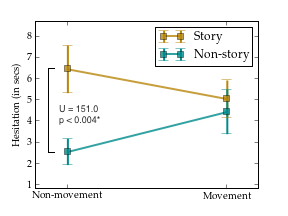
\includegraphics[width=4in]{figures/hexbug/has_story_interaction.png}
      \caption{Interaction of movement x story conditions showing mean hesitation and SD of mean.}
      \label{fig_has_story_interaction}
   \end{figure}
   





Four comparisons of hesitation are of interest: movement vs. non-movement for each of the two story conditions, as well as story vs. non-story for each of the two movement conditions. The results, summarized in Table \ref{table_has_story}, show that there is significant difference in the measured hesitation between story and non-story condition for the non-movement case ($\mu_{story}= 6.45s, \mu_{non\_story}=2.58s; U=151.0, p <0.004$; significant at $\alpha=0.05$ after Bonferroni correction for 4 comparisons). We will return to these results in the discussion section.



\begin{table}
\renewcommand{\arraystretch}{1.3}
\caption{Mean hesitation for Story X Movement}
\label{table_has_story}
\centering
\begin{tabular}{c||c|c|c}
\hline
& Story & Non-story & \specialcell{Mann Whitney\\ U, p}\\
\hline\hline

Movement & 5.05s & 4.44s & \specialcell{$U=281.5$,\\$p<0.384$} \\
\hline
Non-movement & 6.45s & 2.58s & \specialcell{$U=151.0$,\\$p<0.004$*}\\
%\footnote{is this in the table}}\\  %FIXME <--- get damn footnotes to work.
\hline
Mann Whitney U, p & \specialcell{$U=437.5$,\\$p<0.086$} & \specialcell{$U=124.5$,\\$p<0.178$} \\

\hline
\end{tabular}
\end{table}


\subsection{Empathy}


We had hypothesized that subjects with higher trait empathy would hesitate longer in striking the hexbug. (H2) We divided subjects into two equal sized groups of high and low empathy around the median value for each empathy subscale. Of the three subscales, we found  that those with high scores on empathic concern (EC)  hesitated significantly longer ($\mu_{high-EC}=6.39s, \mu_{low-EC}=3.55s; U=900.0, p<0.005;$ significant at $\alpha=0.05$ after Bonferroni correction for 3 comparisons). The other subscales Fantasy (FS) and Personal Distress (PD) do not show any significant changes in hesitation (Table \ref{table_empathy}).

 
\begin{table}
\renewcommand{\arraystretch}{1.3}
\caption{Mean hesitations for high and low empathy subjects for empathy subscales}
\label{table_empathy}
\centering
\begin{tabular}{c||c|c|c}
\hline
IRI Subscale & High Empathy & Low empathy & Mann-Whitney U, p\\
\hline\hline
FS & 5.59s & 4.33s & \specialcell{$U=1230.5$\\,$p<0.385$} \\
\hline
EC &  6.39s & 3.55s & \specialcell{$U=900.0$,\\$p<0.005*$} \\
\hline
PD & 5.56s & 4.26s & \specialcell{$U=1160.5$,\\$p<0.249$} \\
\hline
\end{tabular}
\end{table}



   \begin{figure}[thpb]
      \centering
      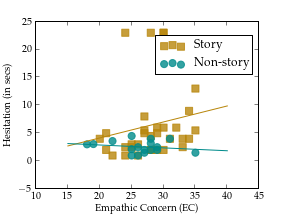
\includegraphics[width=4in]{figures/hexbug/ec_story_no_story_lm.png}
      \caption{Scatter plot of hesitation versus EC for non-movement data colored by story condition. Approximate regression lines are shown for illustrating difference in relationship between EC and hesitation for the story and non-story conditions. }
      \label{fig_ec_story_no_story_lm}
   \end{figure}
   

For the rest of the empathy analysis we look at just the two non-moving conditions (story vs non-story) where we see the greatest difference in the measured interaction. EC is moderately correlated with hesitation in the story condition (Spearman's $\rho=0.37$)  but weakly negatively correlated  (Spearman's $\rho=-0.12$) in the non-story condition (Fig. \ref{fig_ec_story_no_story_lm}).

To understand the effect of interaction of stories with empathic concern, we performed a two-way ANOVA-on-ranks test with Has-Story (Story and Non-Story) and EC as the independent variables and rank-transformed hesitation as the dependent variable. ANOVA-on-ranks showed a significant main effect of has-story ($F(1, 49)=8.92, p < 0.005$) and significant interaction of EC with Has-Story ($F(1, 47)=4.315, p < 0.044$). The significant interaction of EC with story holds even if we consider just the implicit life-stories ($F(1, 31) = 4.20, p < 0.05$)

We found no significant gender effect on subjects' hesitation to strike the robots.

\section{Discussion}
\label{sec_hexbug_discussion}

We hypothesized that hesitation to strike the robots would be greater for implicit life-story conditions compared to non-story conditions (H1). Our results confirm that stories can have an impact on people's reactions to robots. 

Interestingly, we noticed no significant difference in hesitation due to movement. We saw the greatest difference in hesitation between story and non-story for non-moving robots, but the difference became insignificant in the moving case (Fig. \ref{fig_has_story_interaction} ) We have two potential explanations for this. First, we could have been measuring two different types of reactions, depending on whether a subject has a strong aversion to insects or not. Some of the responses in our survey mentioned a dislike for cockroaches or bugs. Because subjects perceived the Hexbug as very insect-like, it is possible that people with low tolerance for insect-like movement reacted differently than people with high tolerance, creating conflicting effects. However, Fig. 3 indicates that there may be a more interesting relationship between story and movement. Another potential explanation is a disappointment of the subjects' behavioral expectations of the robot. Paepcke and Takayama have demonstrated that setting people's expectations low rather than high for a robot's competence leads to less disappointment and more positive evaluation of the robot \cite{paepcke_robot_low_expectations}. Because the Hexbug movements are very simple, it is possible that there was a disconnect between what the subjects believed the robot to be capable of based on our stories, and the behavior of the moving robot they were observing. I will re-examine this effect in when I discuss results from the final study in Chapter X. 

Consistent with our second hypothesis, we showed that those with high empathic concern hesitated more in striking the robot. (H2) This suggests that subjects' hesitation was a result of empathy for the robot. Prior studies in this area have had difficulty distinguishing between emotional hesitation and subjects hesitating for other reasons, for example because they did not want to damage something of perceived value. In our study, if the perceived value of the robot was greater for our moving or story conditions (because people attributed more intelligence or technical sophistication to the robot), this could have led to a similar hesitation effect. However, the fact that we find subjects with greater tendency for empathic concern hesitated more suggests that at least empathy is implicated in the hesitation.

Furthermore, for non-moving robots, we found a positive correlation between empathy and hesitation in the story condition and weak negative correlation for the non-story condition. Moreover, our analysis shows that there is significant interaction between empathic concern and stories on hesitation. These findings support our hypothesis that the effect of stories on hesitation is more pronounced for subjects with high trait empathy scores, as opposed to low (H3). This suggests that stories engender empathy, which results in hesitation. Adding descriptive color to our analysis, one question in our post-experiment survey asked subjects to describe in their own words why they hesitated. Many of our subjects used empathic terms to explain their hesitation, for example ``I had sympathy with him after reading his profile because I am also here in the Lab for a few month. [\emph{sic}]''

A study conducted by Rosenthal-von der P{\"u}tten et al., in which subjects watched videos of robots, showed a correlation between subjects' fantasy scores and their responses to the robots being mistreated \cite{rosenthal_emotional_reaction}. While this study may not be directly comparable to ours in many aspects, it is interesting that our study finds subjects' behavior to correlate with empathic concern, rather than fantasy. The fact that our subjects fell into a different category on the Interpersonal Reactivity Index indicates that we could be dealing with a different type of empathy. Further research may prove to support the suggestion that there is a divide between virtual and physical in how humans perceive and respond to robots \cite{bainbridge_robot_presence}, and also that emotional reactions to physical robots are not just guided by fantasy and imagination.


% momentum quote: “It's not who you think you are that holds you back it's who you think you're not.”




\chapter{Construction of a Sound Robot}
\label{chap_design}

In the last chapter, I showed that a toy robot with a fictional back story could elicit empathy. Now, I will describe the design and construction of a zoomorphic social robot that has the ability to autonomously create its own life story. The robot can learn to mimic sounds it hears and improve its imitations with repetition. 



   \begin{figure}[thpb]
      \centering
      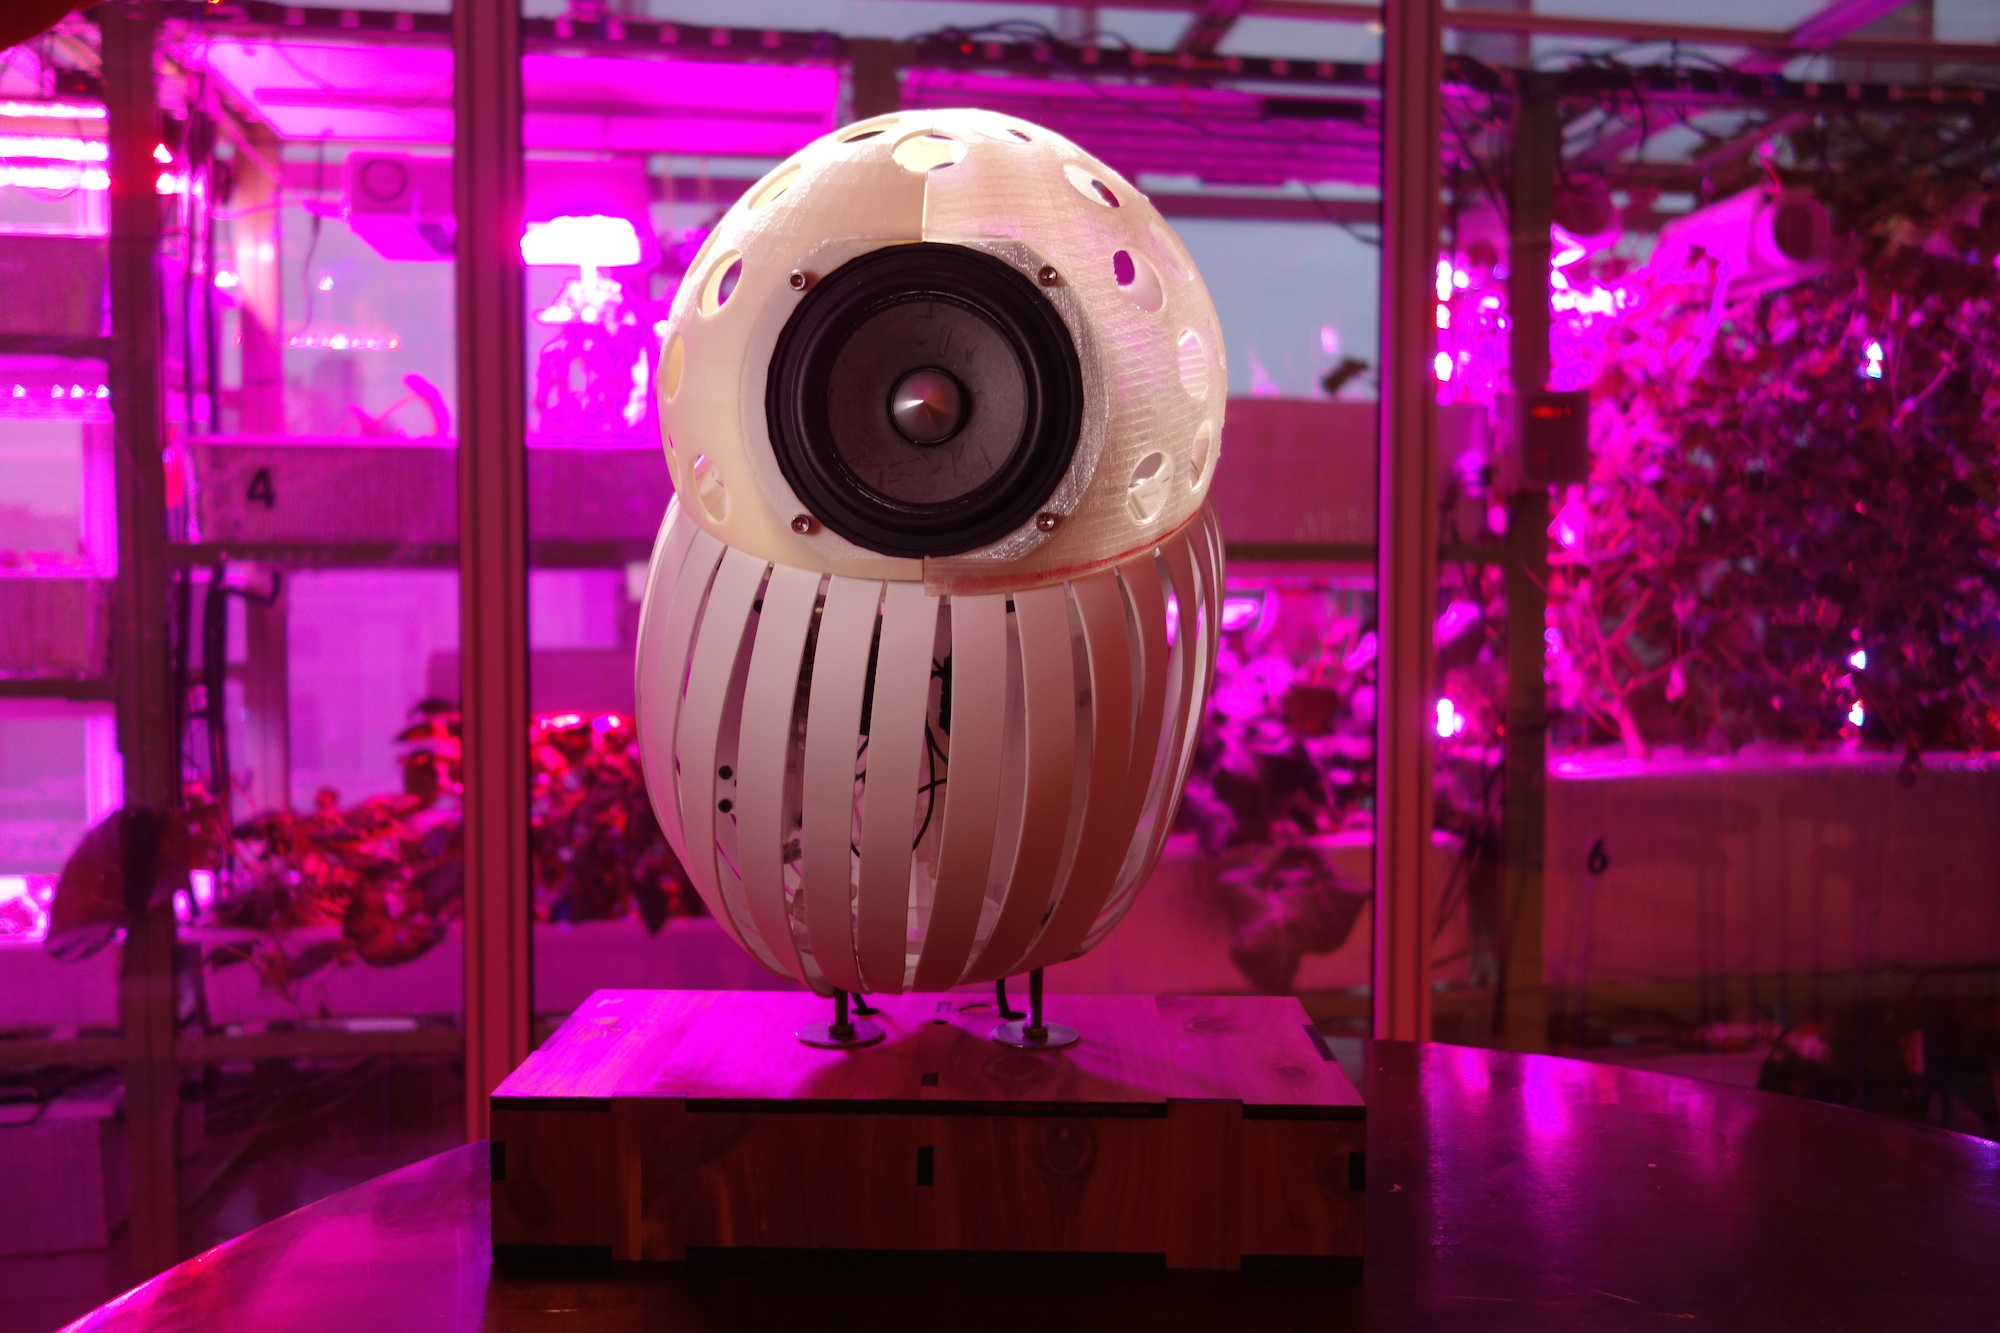
\includegraphics[width=4.6in]{figures/design/parrot_purple.JPG}
      \caption{Ewol the Electric Owl, the sound robot described in this chapter}
      \label{fig_parrot_purple}
   \end{figure}
   

\section{Why a Sound Robot?}

An important design goal for a life-story robot is that it should experience the world in ways we do and change perceptibly from that experience. A sound robot has certain properties that make it attractive for the purpose of this thesis.  Sound allows for human oriented perception that is rich in information ranging from environmental sounds, to thoughts as expressed as words, taking in along the way emotions and speech patterns unique to individuals. Recent advances in technologies such as sound localization, speaker identification, and particularly speech recognition, allow the construction of a robot that can obtain salient information from sound. 

A sound based robot can also be optionally ambient, that is to say, if needed it can experience the world by being merely present in an environment without requiring direct human intervention for the experiences. This allows the robot to have experiences autonomously over long time periods. 

A sound robot can make use of a familiar interaction model, namely how humans typically interact with avian pets such as parrots. People's expectations of intelligence and emotional expression are lower for birds compared to cats or dogs which makes design goals for a bird-like robot more modest. In addition to establishing low expectations for interaction, utilizing the avian companion model solves a thorny problem for robots: power distribution. A robot of the avian persuasion can be plausibly restricted to sitting on a perch which would allow for power and data connections. 


\section{Design Process}

   \begin{figure}[thpb]
      \centering
      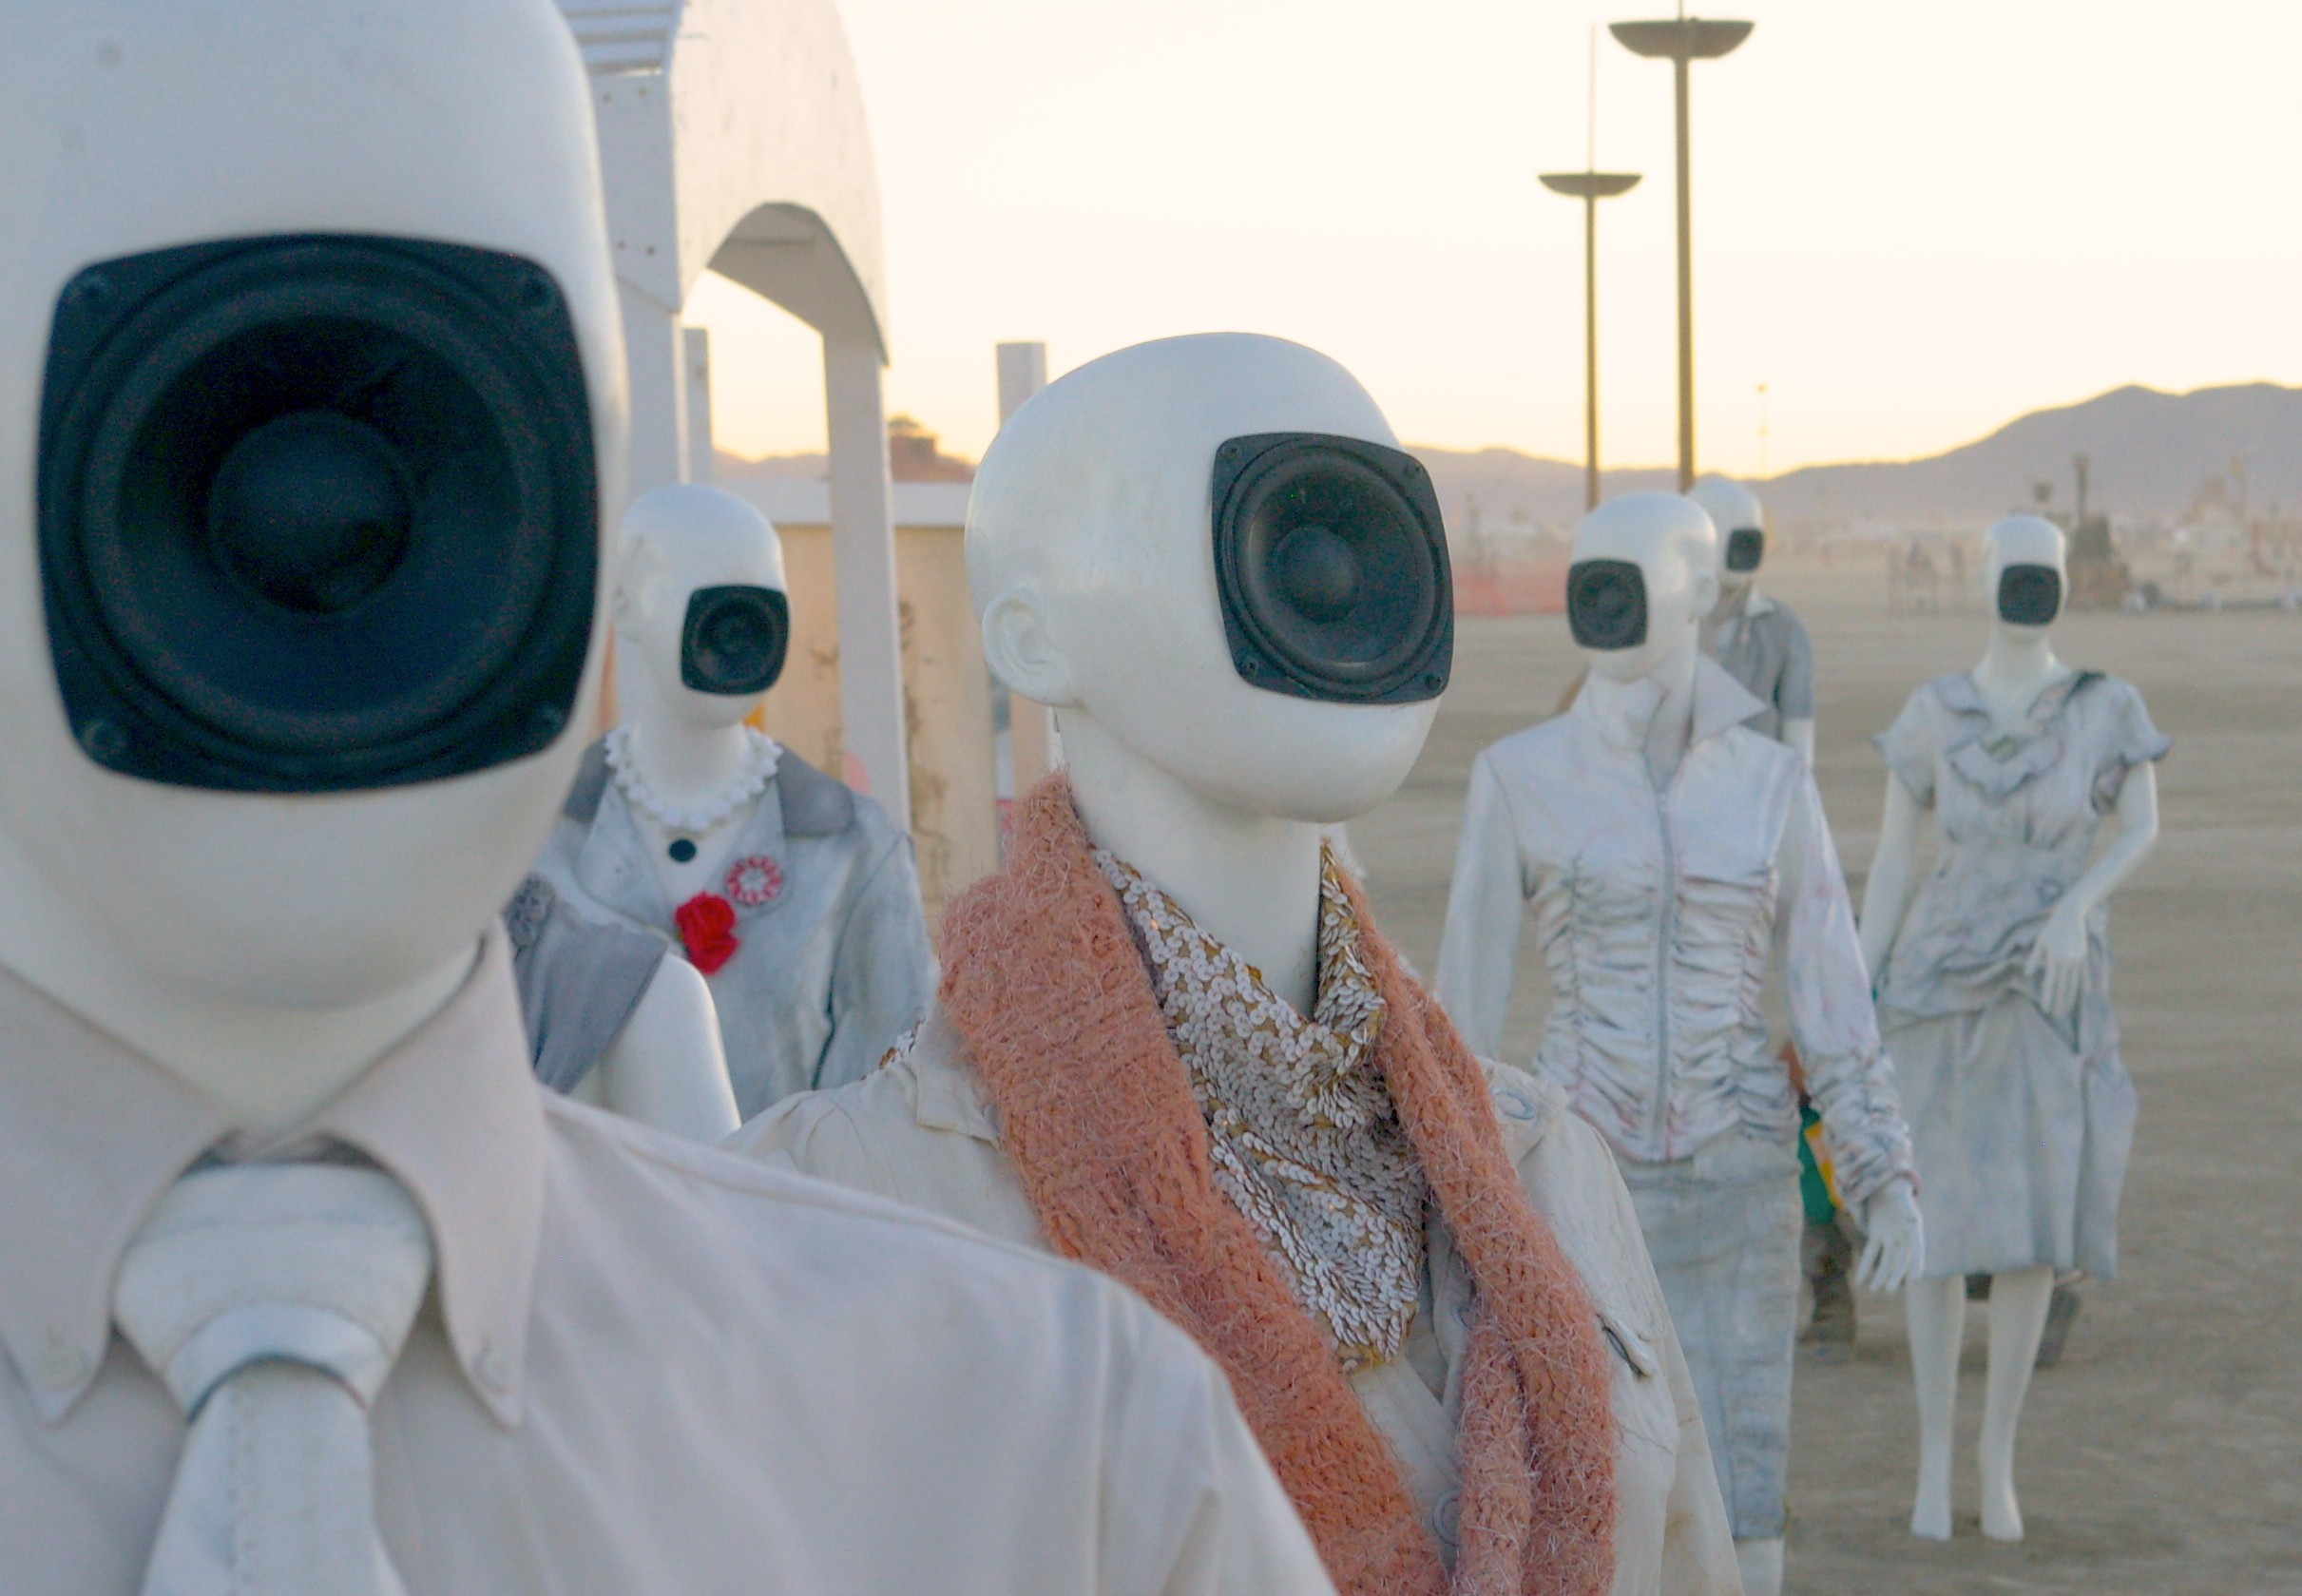
\includegraphics[width=4.6in]{figures/design/burning_man_speakers_sm.jpg}
      \caption{Mannequins with speakers by unknown artist at Burning Man 2010, the inspiration for the speaker-as-face design for my robot}
      \label{fig_burning_man_speakers_sm}
   \end{figure}
   



   \begin{figure}[thpb]
      \centering
      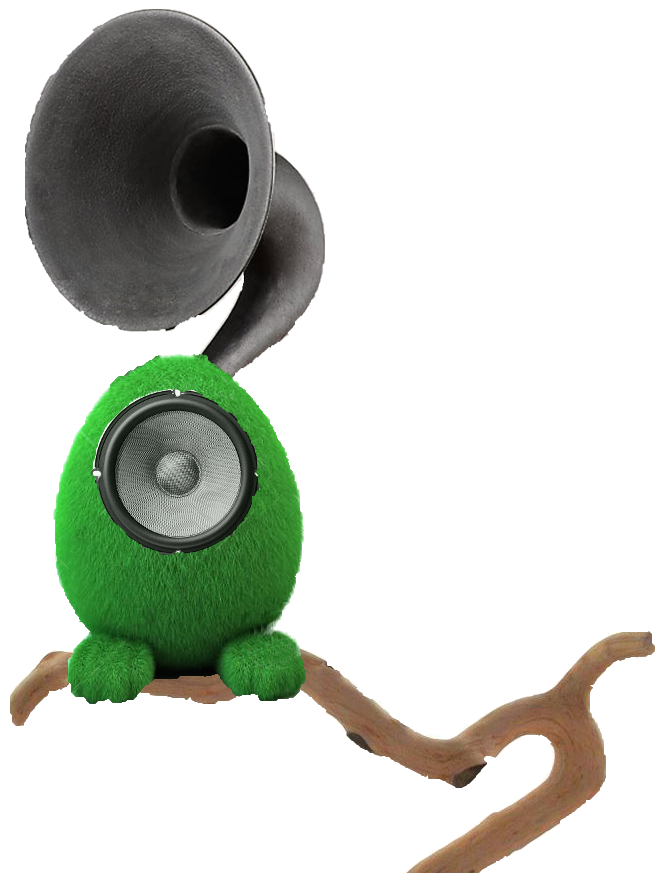
\includegraphics[width=3in]{figures/design/green_blob2.png}
      \caption{Early design for the robot with exaggerated sound features}
      \label{fig_green_blob2}
   \end{figure}


   \begin{figure}[thpb]
      \centering
      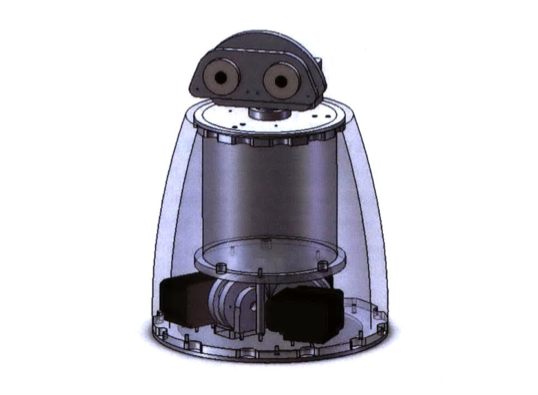
\includegraphics[width=4in]{figures/design/tofu_design.png}
      \caption{Ryan Wistort's Tofu showing squash stretch mechanism \cite{wistort_tofu_draw}. Three servos in the base of the robot pulled on cables that compressed a central column of bedding foam. Tofu's motion and mechanism inspired the design of my sound robot.}
      \label{fig_tofu_design}
   \end{figure}


  \begin{figure}[thpb]
      \centering
      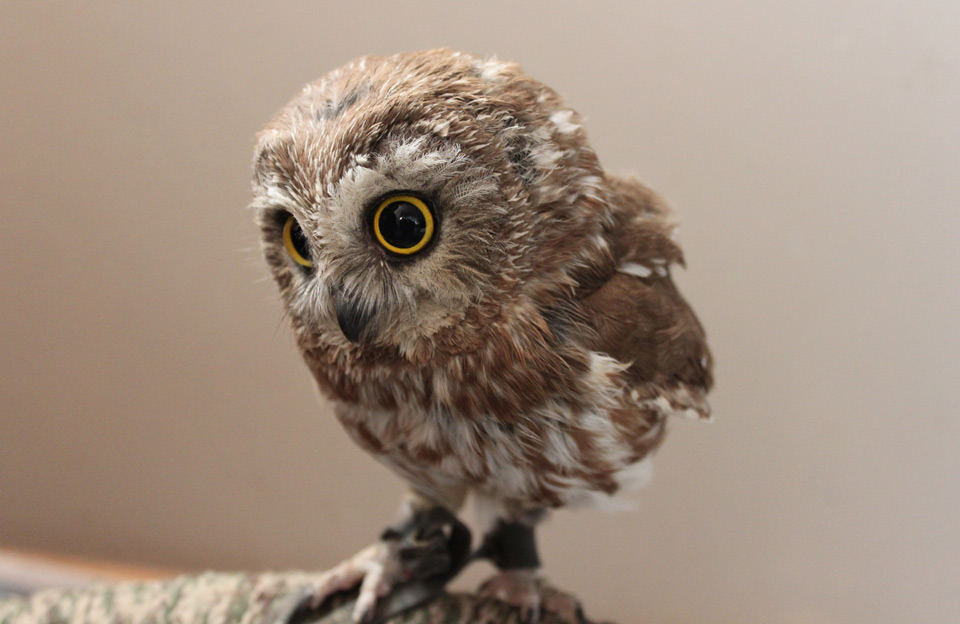
\includegraphics[width=4.6in]{figures/design/owl_inspiration.jpg}
      \caption{Juvenile owl used as an inspiration for the sound robot's form design.}
      \label{fig_owl_inspiration}
   \end{figure}

One of the primary physical design goals was to indicate through visual clues that the robot supported only sound based interaction. To that end, the robot should have exaggerated sound features and, rather unusually for social robots, no discernible eyes. Moreover, to suggest a parrot-like interaction, its form and movement should evoke those of a bird. 

Figure \ref{fig_green_blob2} shows my initial design for the sound robot. The body is based around a blob shape that can squash and stretch much like Wistort's Tofu robot (See Figure \ref{fig_tofu_design}) \cite{wistort_tofu_draw}. The green fur covering is evocative of a parrot. Inspired by a moving work of art which used speakers for faces of mannequins (Figure \ref{fig_burning_man_speakers_sm}), the main feature of the robot's face is a speaker. A large gramophone horn stands in for an over-sized ear trumpet. The overall hybrid mechanical organic form seemed suitable for a robot that is aspiring to be life-like. The whole robot is mounted on a branch which route power and data. 

Life-like motion, as discussed earlier, is a key contributor to robot's believability.\marginpar{

      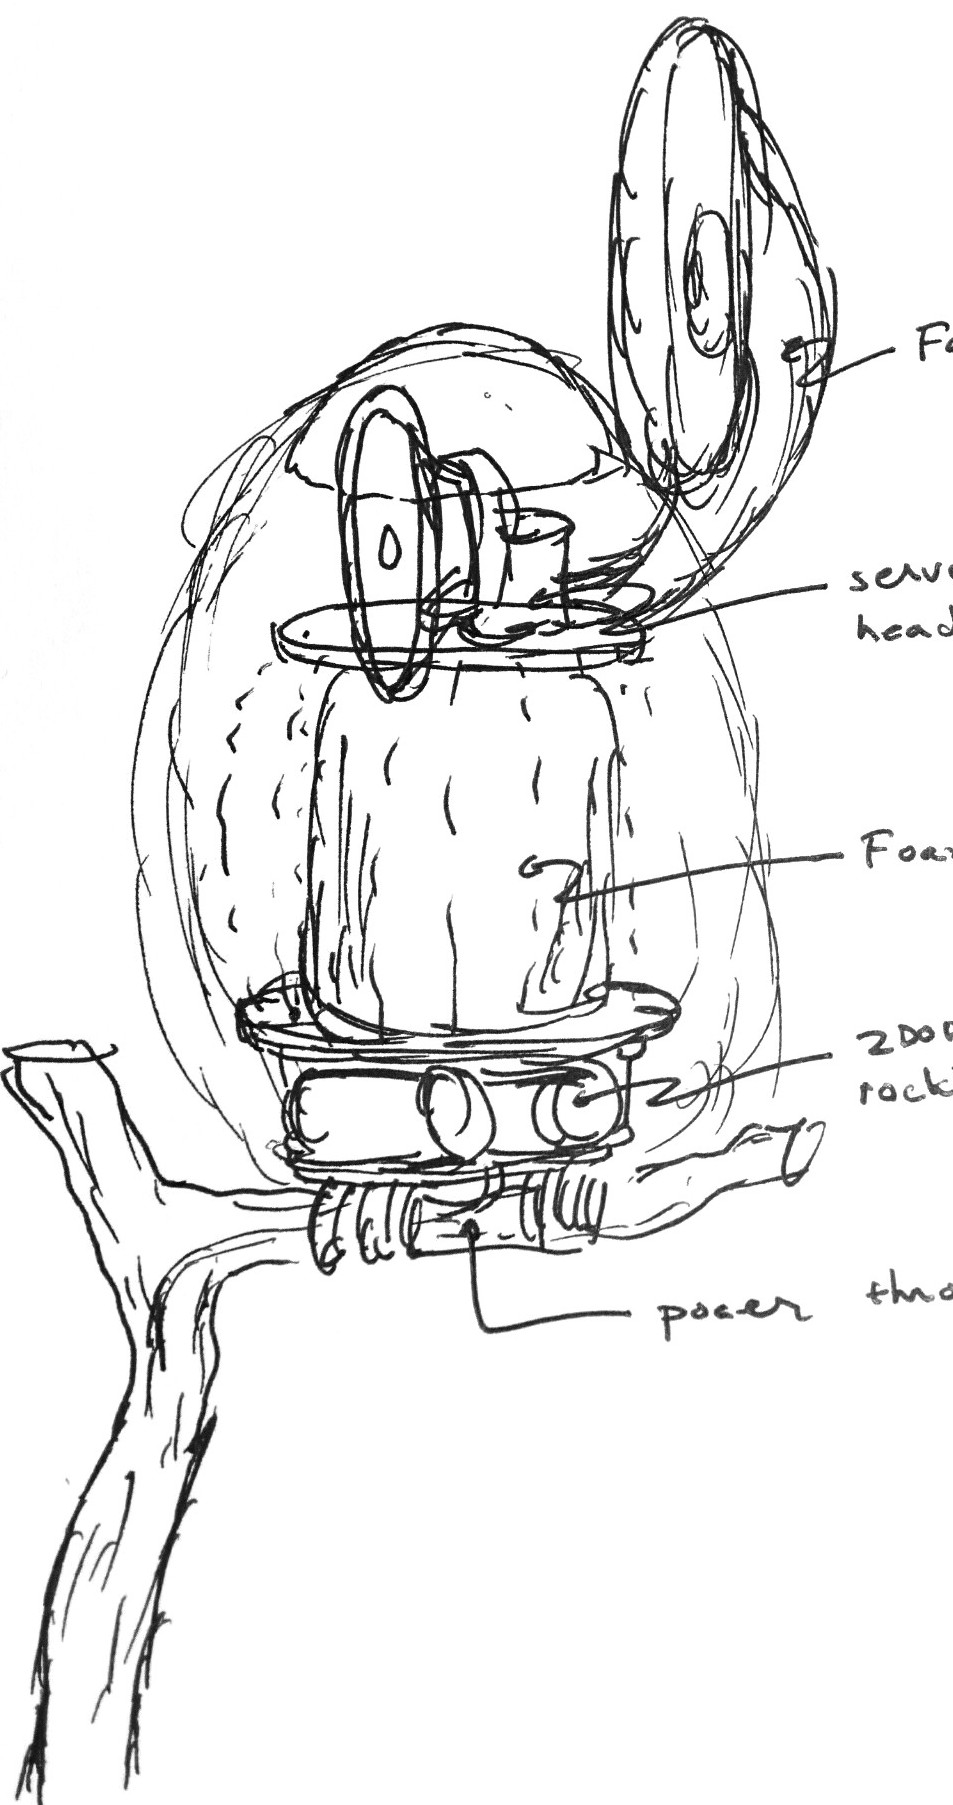
\includegraphics[width=\marginparwidth]{figures/design/hand_drawn_green_blob2.jpg}
      Sketch of potential mechanisms.
      %\caption{Juvenile owl used as an inspiration for the sound robot's form design.}
      \label{fig_design_hand_drawn}

   

} In this design, the robot would be able to do a breathing motion while idling, puff up when it is speaking, rock side to side to suggest excitement, lean forward to show interest, lean back to indicate fear, turn its head to look around, and cock its head to listen. Much like the use of ears in other social robots, the independent movement of the trumpet could be used for expressing affect. 

While revising this initial design, for aesthetic reasons, I changed the form to be closer to that of a juvenile owl (Figure \ref{fig_owl_inspiration}) than a parrot. The trumpet was sacrificed for simplicity of construction. In response to feedback from early testing, the robot got a foam skin that exposed the internal structure instead of fur, shifting the overall design to be more mechanical than organic. 


\section{Physical Construction}

The mechanism for the sound robot is fairly simple \footnote{I worked on the physical construction with Andres Salgado-Bierman, an undergraduate researcher. Andres was responsible for an early version of the linear actuator and the skin for the robot. I am indebted to Andres for his help, and also to Arthur Preton, Matt Carney, Young Dae and Harald Quintas-Baz for feedback on the mechanical design.}. The robot has four degrees of freedom, three of which are used for animating the body and one for turning the head. 

\subsection{Body}

The body of the robot consists of two parallel plates connected by three linear actuators. Extensions or contractions of the actuators can translate the plates up and down, or pitch forward and backward, or roll left and right. As the plates move relative to each other, they stretch or compress a foam skin changing the apparent shape and size of the body while keeping its volume constant. 

The bottom plate is mounted at an angle to the ground so that the axis of the body tilts forward at rest. Due to this forward tilt, an extension of the plates causes the robot to stretch forward towards the user, and a retraction to shrink away allowing it to express interest or fear. 






   \begin{figure}[thpb]
      \centering
      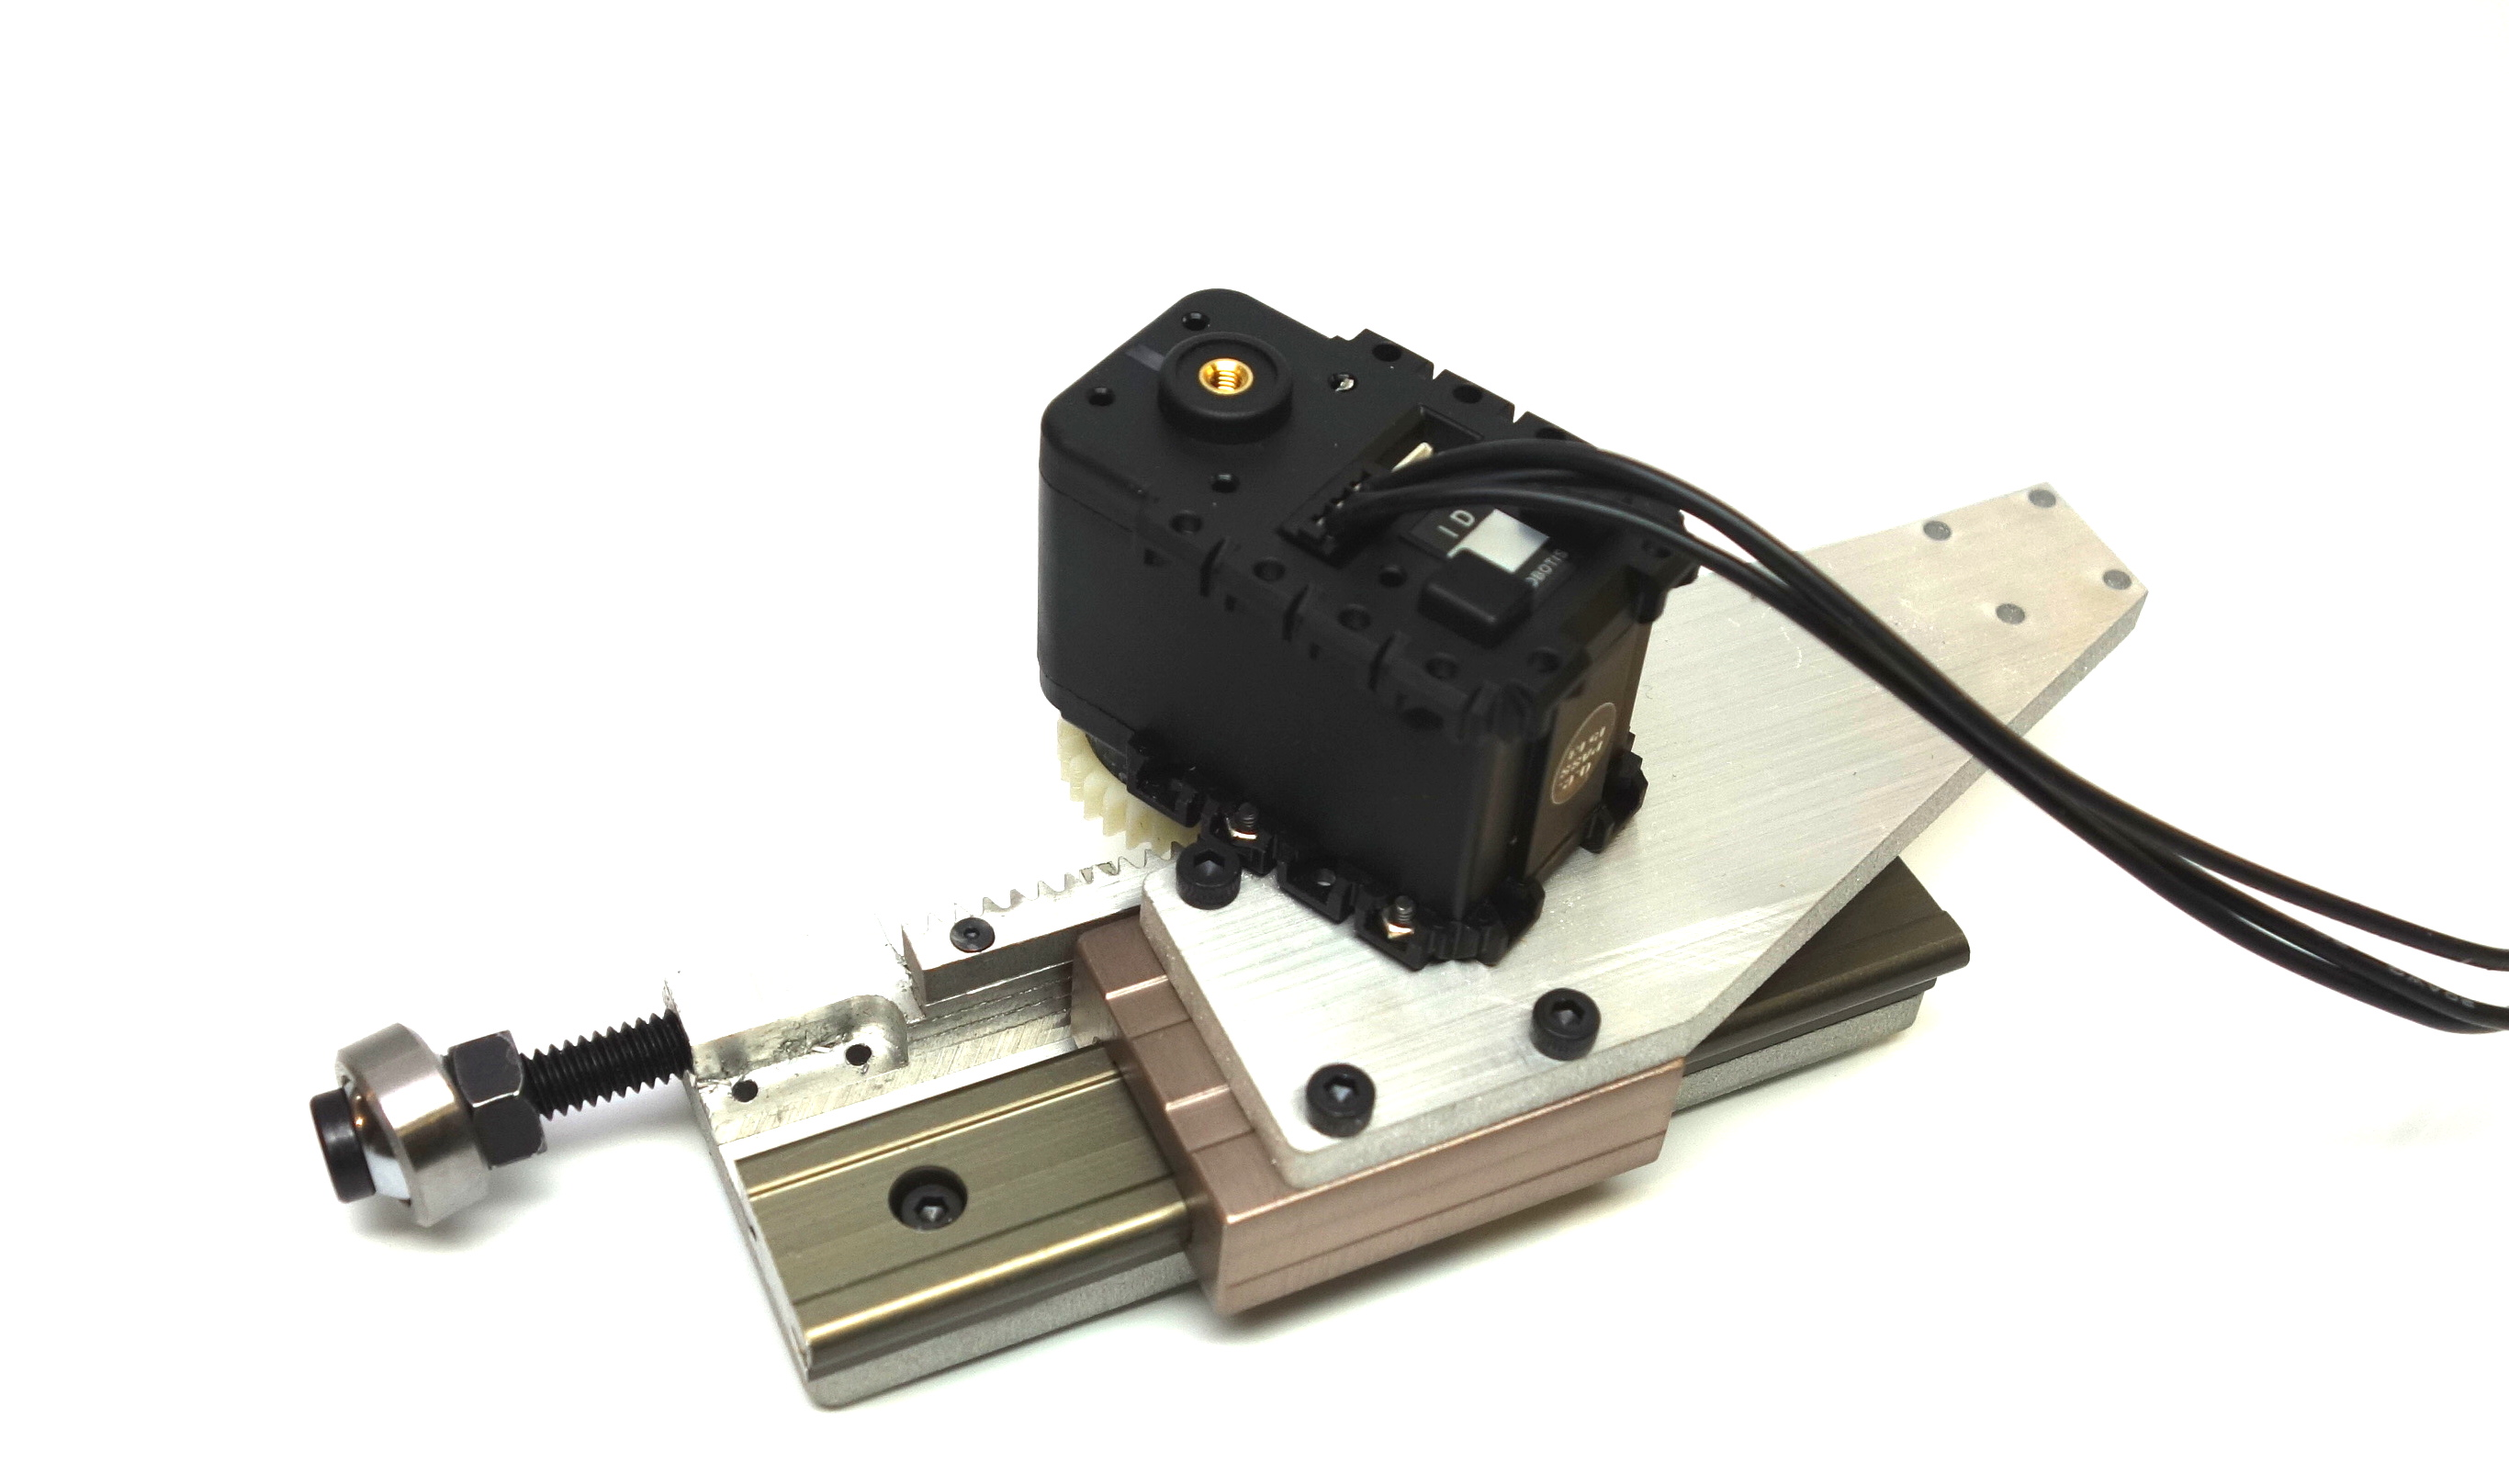
\includegraphics[width=4.6in]{figures/design/actuator.jpg}
      \caption{Detail of the linear actuator used to create squash-stretch animation in the robot's body}
      \label{fig_design_actuator}
   \end{figure}




   \begin{figure}[thpb]
      \centering
      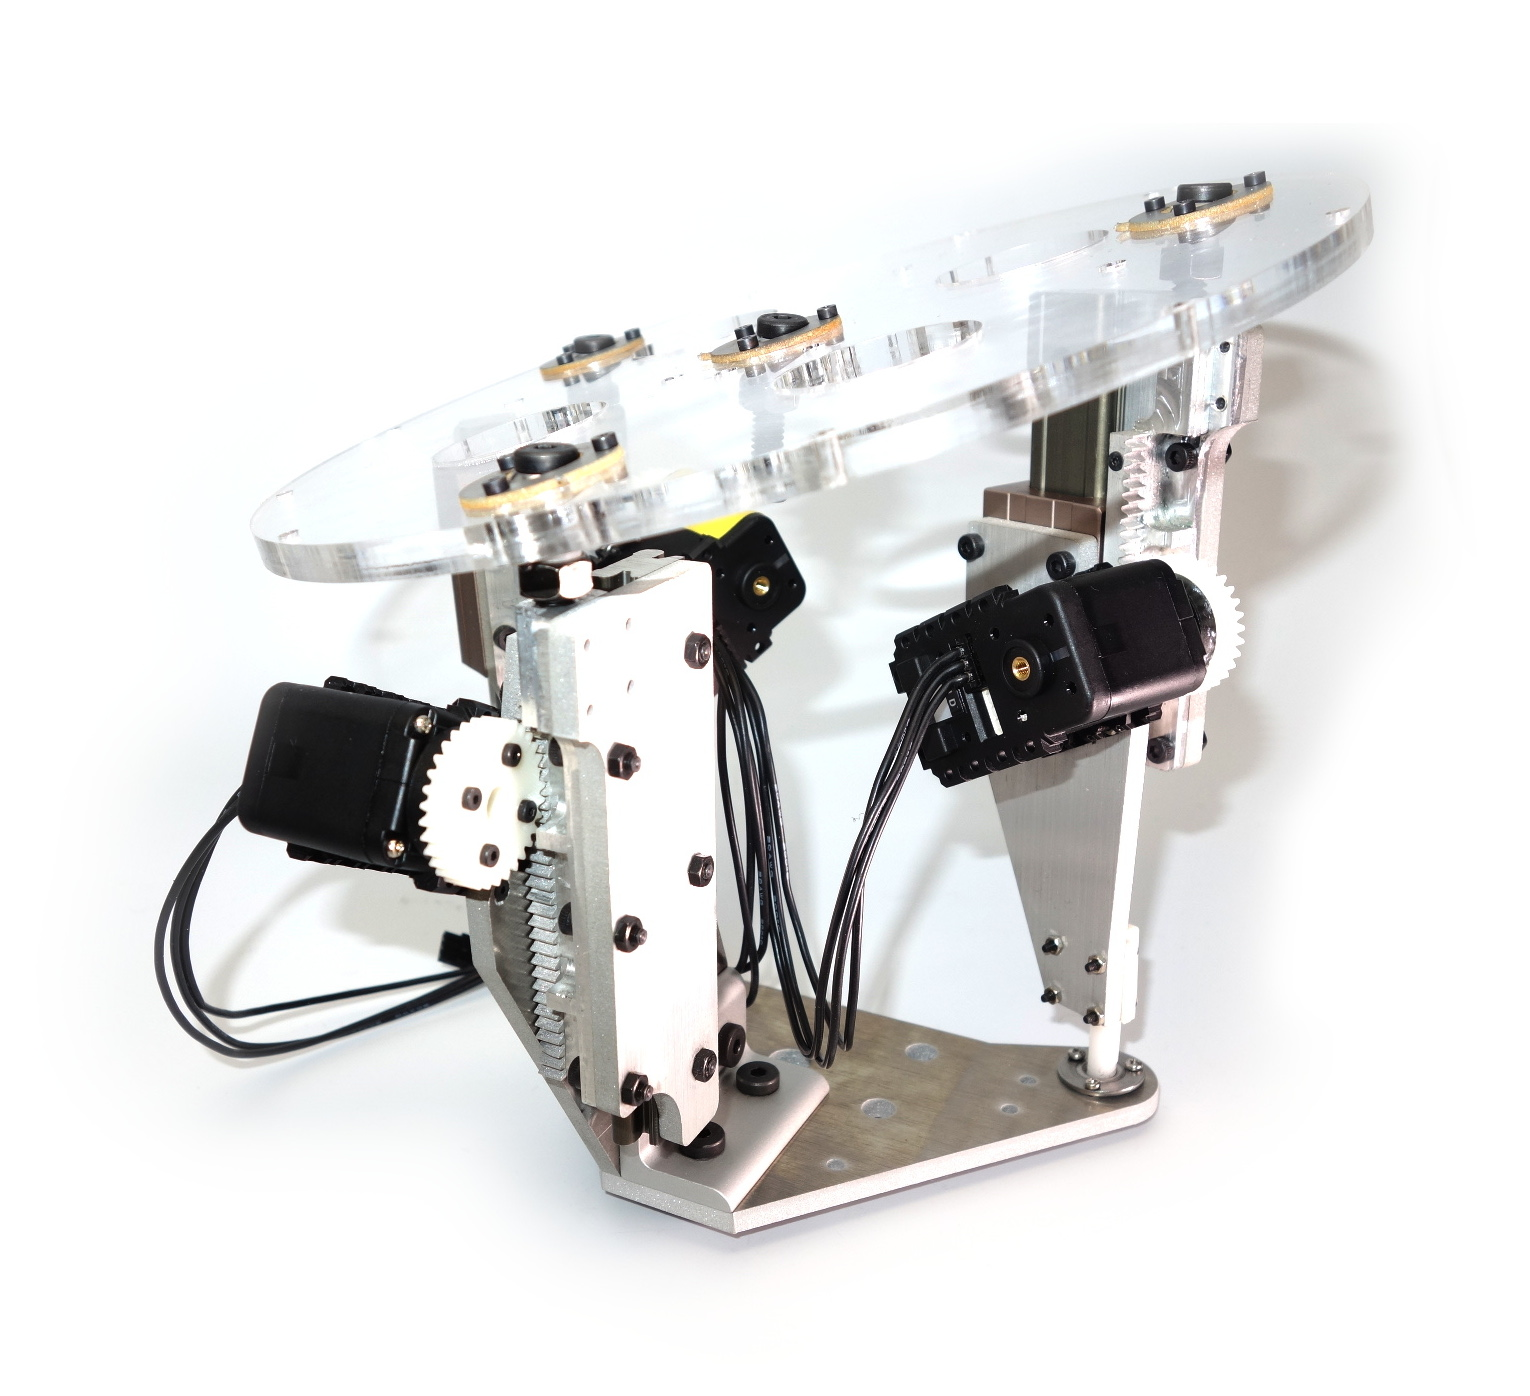
\includegraphics[width=4.6in]{figures/design/body_assem2.jpeg}
      \caption{Body assembly showing the top and bottom plates separated by the actuators}
      \label{fig_design_body_assem}
   \end{figure}





The linear actuators use a rack-and-pinion mechanism to translate the rotation of the motors into linear motion.\marginpar{

      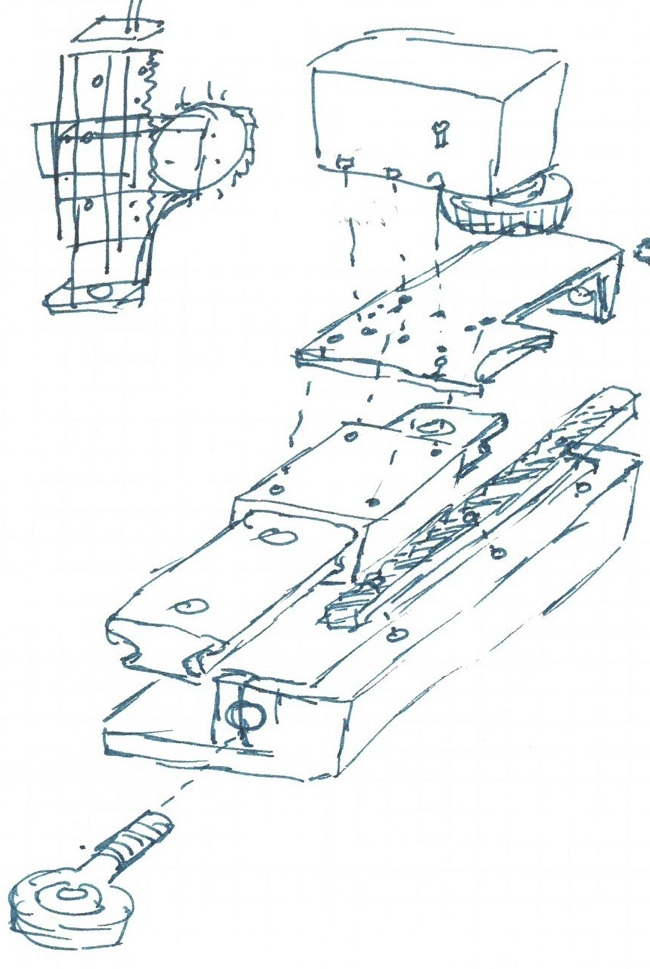
\includegraphics[width=\marginparwidth]{figures/design/linear_bearing_me_sketch.jpg}
      Sketch used as starting point for CAD drawing.
      %\caption{Juvenile owl used as an inspiration for the sound robot's form design.}
      \label{fig_design_linear_bearing}

   

} I made the frame and power transmission mechanism out of stock 6061 aluminum using a combination of waterjet and CNC. Off-the-shelf linear bearings constrain the motion to only one degree of freedom. Ball and swivel bearings connect each actuator to the plates above and below, which allows the plates to tilt relative to the actuator. Gravity preloads the pinion, so there is no backlash during normal operation. I used Dynamixel AX-12A servos for the motors, due to the absolute position control they provide over a serial bus. 



   \begin{figure}[thpb]
      \centering
      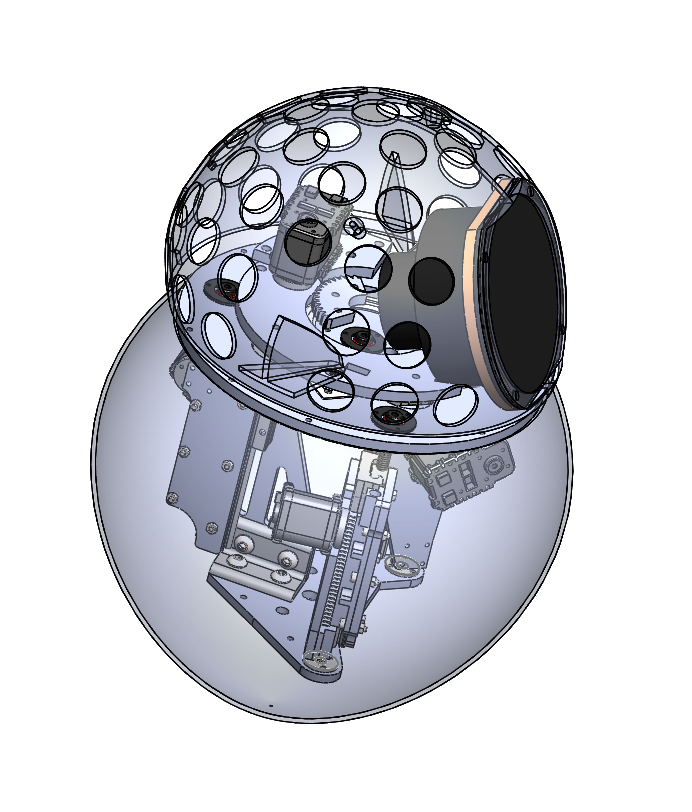
\includegraphics[width=4.6in]{figures/design/solidworks_body.png}
      \caption{CAD Drawings of my robot showing the actuators connecting the body plates. Head shows the speaker assembly and the rotation servo}
      \label{fig_design_solidworks}
   \end{figure}



The head, mounted on turntable bolted to the top plate of the body, can rotate through 120 degrees using another AX-12 servo. The forward tilt of the body of the robot puts the head on a canted axis, which creates a sweeping motion for the rotation of the head. Laser cut acrylic mounts in the head hold up a speaker, a full spectrum 4" Tang Tang Band W4­1320SJ driver, which forms the main visible feature of the face. 

\subsection{Skin}

The body of the robot is sheathed in bands of white craft foam that come to a point at the tail of the robot. The foam strips bellow out when the body plates contract creating the impression of organic mass. The head of the robot is encased in a 3D printed dome perforated with holes to reduce weight and cost. The overall form is suggestive of a juvenile owl. The gaps in the white foam and dome expose the internal mechanical structure of transparent acrylic and aluminum scaffolding. I intended to cover the foam and the dome with fur or feather boa to make the appearance more creature-like. However,  reaction to the accidental Bauhaus aesthetic of the robot was positive, so I decided to keep the robot in its semi-mechanical semi-organic form. 

\subsection{Electronics}

The electronics of the robot consists of a motor controller and an amplifier. The Dynamixel servos from the actuators and the head connect via daisy chained serial lines to an Arbotix controller located in the base of the robot. The controller, based on a AVR AtMega processor, talks to an off-board computer using a FTDI serial connection. The servos have on-board electronics for feedback position control so the main task of the controller is to provide power to the servos and adapt the servo serial communication to serial USB. 

The speaker is driven by a Sure TDA7492 Class D audio amplifier located alongside the motor controller. The amplifier routes the audio output of the computer to the robot speaker. A USB microphone provides audio input. The microphone array of a disassembled Microsoft Kinect provided audio localization but the feature was not used in the study. 

For the validation study, I made a fake memory card reader which consists of a 3D printed device that holds a memory stick shaped acrylic against a limit switch. The motor controller also provides an interface for digital sensing which is used to sense the presence of the memory stick.

The overall cost of materials for the robot came to \$815 USD with the servos being the most expensive item at \$180 USD for the 4 motors. 

\section{Software}

 In the last section, I described how the robot moves via the operation of four servos. Here, I will describe the action system that uses those servos to create believable motion, the cognition system which acts on the world by requesting actions of the action system, and the perception system through which cognition senses the world. These systems are connected together over Robot Operating System (ROS) \cite{ros}. I wrote these software components that run on the computer in Python. 


\subsection{Action System}


   \begin{figure}[thpb]
      \centering
      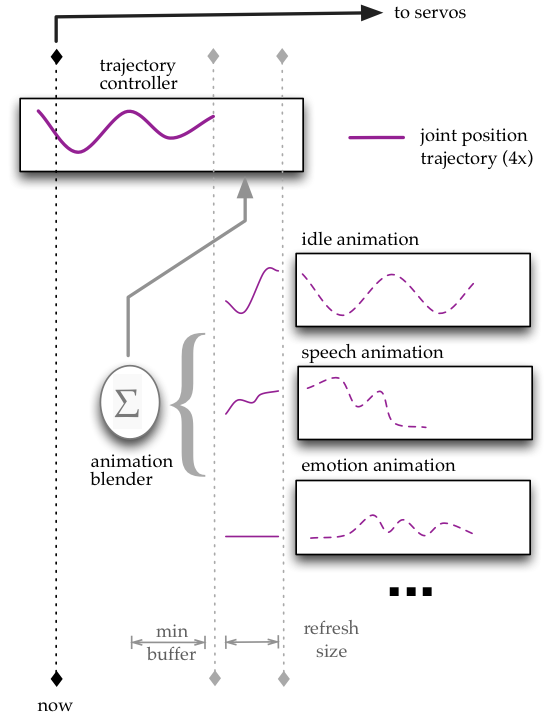
\includegraphics[width=4in]{figures/design/animation_system.png}
      \caption{Diagram showing the different components of the robot's action system. The trajectory controller sends position to the servos from a buffer of joint positions. When the buffer falls below a minimum threshold, the action system refreshes the buffer with blended chunks of trajectories from each submodule. The submodules maintain their own buffer of future trajectories. The buffer sizes are tuned to trade off reliable smoothness of animation with responsiveness.}
      \label{fig_animation_system}
   \end{figure}


The action system is the most complex part of the software, consisting of many threads of execution running in parallel (See Figure \ref{fig_animation_system}). At the lowest level of action is a feedback control loop running on each Dynamixel servo that, given a target position, will hold the motor at that position. Firmware on the Arbotix controller relays commands received over the serial link from the computer to the servos in the actuators and in the head.

On the computer, the Joint Trajectory Controller\footnote{I modified an existing controller by Vanadium Labs to allow the continuous buffering needed for smooth motion.} continuously sends target positions to the servos over the serial link. As an input, this controller takes in a trajectory, that is a series of positions for all of the robot's joints over a time window. On every clock tick, the controller interpolates positions and velocities and sends updates for the target position to the servos. To avoid discontinuity in the trajectory and keep the motion smooth, the controller maintains a buffer of joint positions. The action module, which is responsible for generating the joint trajectories, sends a new trajectory if the buffer falls below a minimum threshold. 

The action module forms the core of the action system. The module consists of separate submodules for each kind of action all running independently in parallel. For instance, an Idle Action submodule generates a breathing motion for the robot. Irrespective of other co-occuring actions, it creates a gentle expansion and contraction of the front of the robot. When the robot speaks, the Speaking Action submodule generates a motion trajectory to puff up the `chest' based on the energy of the utterance. There exist other submodules for producing emotionally expressive motions, for looking around, for playing back prerecorded animations, and so on. Each submodule maintains its own buffer of trajectories. When the controller's buffer gets low, the action module asks for small chunk of trajectories from each submodule, blends them together and then ships them over to the controller to extend its buffer. The blending allows the robot to continue breathing while speaking and turning its head. 

The action system works autonomously unless the cognition system requests a change in behavior. Each submodule of the action module exposes an interface over ROS so that cognition can trigger actions or changes in behavior of the submodules.

\subsection{Cognition System}

The cognition system reacts to the world as seen through the perception system and expresses itself through the action modules.  

The main task of cognition system for this robot is learning to speak from hearing people talk to it, and simply overhearing conversations. Per my thesis, the utterances the robot makes should be suggestive of the sounds it heard and engage the listener in reconstructing its experiences. The learning should occur quickly enough so that a casual human teacher would remain engaged through a training session. There is also the problem of people discovering the scope of the robot's experience: how would a new user of the robot know what it can say? While occasional random utterances of previously heard sounds wouldn't be entirely unlike the behavior of parrots, it would make the discovery of the robot's experience challenging. To help an user probe and explore the robot's experience, the robot should learn not just phrases but responses to phrases. 

There are two kinds of learning mechanism in the cognition system. With the first, the robot gets progressively better at mimicking a phrase it hears repeatedly; the second is how it learns responses to phrases. 

The first kind of learning is achieved through a simple pseudo-development mechanism\footnote{As an initial approach, I tried to approximate sounds heard by controlling the parameters of a simple vocal apparatus of sine wave generators. A Nelder Mead based gradient descent on the distance between the sound produced and target sound in a MFCC feature space, drives the utterances closer to target sound. While this mechanism, inspired by neurological understanding of song generation in zebra finches \cite{doya_computational_model_songbird}, is more biologically plausible, the optimization required many iterations in practice and was too slow to be useful for my application.} . A speech recognition engine in the cloud translates sounds from the environment into text where possible. The robot then repeats what it heard using a text-to-speech engine with some distortion to make its speech sound bird-like. A low-pass filter cuts off the high frequency sounds and the resulting sound is then pitch shifted up. The theshold and the degree of pitch shifting depends on the level of distortion ($threshold = 500 + (3500 * (1 - distortion))$; $shift percentage = 700 + (900 * distortion))$). The cognition system maintains a memory of all the phrases it heard and their frequency of repetition. As a phrase is heard more often, the distortion in the reproduction is progressively lowered making the utterance clearer. However, reproduction is never perfect and that combined with errors in speech recognition leaves some ambiguity about the utterance. The ambiguity was deliberate to engage the user in reconstructing the sound. 

The learning of responses to phrases is done using hebbian learning. The robot keeps track of phrases that frequently co-occur in conversations directed to it or that it overhears. For instance, the question ``What's up?'' might be followed by ``Not much'' or, perhaps more reflective of the exigencies of a center of learning and research, ``Aargh! I have a paper due.'' From this exchange the cognition system will maintain a link between ``What's up?'' and the example follow-on phrases. The robot will subsequently utter a follow-on phrase when it hears the antecedent. If there are many candidate phrases, cognition picks one with a probability based on the strength of association with the antecedent. 

The cognition also triggers various animations based on its state. For example, when it fails to transcribe speech, it triggers a mild head shaking animation through the action system. When cognition perceives an user is starting to talk to the robot, it causes the body to lean forward to express interest.  

For the purpose of the validation study, cognition also handled behavior associated with memory loss. When the memory of the robot is erased, it engaged in a distressed thrashing animation followed by a state where it responded to spoken phrases only by beeping. 

Lastly, there is a hidden command mode in the cognition system used for debugging and low level control of the robot. On hearing a key phrase, ``Joshua'', the robot transitions into this access mode. Then, using voice command an user can ask the robot to shutdown, to perform backups of memory, or to play a game of chess. 

\subsection{Perception System}

Being a sound robot, the primary perception of the robot is through the microphone. The robot looks for high energy in the audio stream and starts recording until pause at which point, it sends the recorded buffer to be converted to text using Google's speech recognition API. The cognition system responds to energy of the sound and the generated text. There is also mechanism for locating direction of sound using Microsoft Kinect's microphone array.

For the validation study, there were two more sources of input. An off-board hidden camera detected if there was  a face in the robot's view using a Haar cascade classification of the video stream. This mechanism was used to selectively engage the robot during a conversation with a study participant and to prevent the robot from interrupting the study with its utterances. In addition, the robot is wired to a limit sensor that detects the presence of a fake memory card. I will discuss the usage of these in the next chapter. 



In the next chapter, we will look at the results of human subject studies to determine people's perception of the robot, and particularly its ability to elicit empathy.














% 4-10 home
% 4-11 home
% 4-14 work


\chapter{Pilot Study}
\label{chap_pilot}

\section{Summary}

In the last chapter, I described how I designed and built a robot that creates its own life story by changing from experiencing sound. Here, I will describe the first steps I took towards testing people's reaction to the robot\footnote{I am grateful to Kate Darling for help with conducting the pilot and particularly for shooting and editing the video of the robot's story.}. This initial testing help refine the design of the controlled validation study that I will discuss in the next chapter. Moreover, the process of testing was helpful for me in characterizing implicit life-stories. The experience recorded here may be useful for future designers of similar robots or studies. 

\section{Method}

28 subjects, recruited locally, were given an opportunity to interact with the sound robot. They were also shown a short video montage of the robot's progress of learning to imitate sounds in various environments such as around the lab, in a public corridor or at a local bar. After the video and the interaction, they were instructed to erase the robot's memory. If they chose to do so, the robot showed distress and then reverted to a non-talking state. Much like the hexbug study, I expected that empathy for the robot would make the participants reluctant to cause harm to it. Afterwards, I conducted an informal interview with the participants of their experience. During the interview I asked them to choose words to describe their impression of the robot and in particular if they felt bad about the robot losing its memory. 

\section{Results and Discussion}

The subjects liked the robot and generally described it as friendly and pleasant. Majority of the participants thought of the robot as interactive, alive and conscious while still regarding it as mostly mechanical.  I will go into more details of the impression of the robot in the main study but based on this pilot, I was satisfied that the physical design and movement of the robot was adequate to trigger a social model and to suggest that it had a mind. 

However, most participants didn't feel bad about the robot losing it's memory. The interviews revealed two reasons for it: primarily the participants didn't believe that memory was actually getting erased and some were not moved by the robot's story. 

\subsection{Convincing memory loss}

A convincing and emotionally provocative memory erasure procedure required some iterations. In the initial experiment design, I had the participants press and hold down a button to erase the robot's memory. While the button was being held, the robot would thrash around making distressed sound which suggested regression of knowledge and ability: the robot would start by ``Hello robot. How are you.'' which would devolve into an increasingly mechanical ``hello hello'' and finally just beeps. I reasoned that out of empathy for the robot, a participant would let go of the button a few seconds into the procedure. However, participants held on and watched the process of the robot's simulated memory loss till the very end. I assumed that they were too shocked to take the deliberate action of letting go of the button. Accordingly, I changed the procedure to have the participants click on the button repeatedly; each click playing back a segment of animation and vocalization suggesting that additional chunks of the robot's memory was being last. Most participants clicked on the button all the way to the end of the animation sequence and then some more. When asked, participants said that they didn't actually believe a button press was erasing the robot's memory. I changed the erasure procedure to the participant extracting a fake memory card from a card reader and then cutting up the card with shears. I found that changing the subject population to an older and non technical pool recruited from Craigslist, rather than Media Lab students, also helped address the incredulity about memory erasure.

\subsection{Implicit life-story of the robot}

The problems with the robot's story, as told through vignettes, was more nuanced. Initial videos showed that the robot was being deliberately trained by various people to repeat arbitrary phrases such as  ``thundercloud.'' Based on feedback from the pilot, I iterated on the robot's back story portrayed in the video. In the end, the video showed the robot learning to say more meaningful phrases such as ``good morning'' from overhearing conversations and casual interactions. What follows is what I learned from informal interviews with participants while iterating on the video presentation of the robot's story. These lessons are not supported by quantitative data but may be useful as a source of hypotheses to test with controlled studies and as guidelines for future designers of similar robots. 

\subsubsection{Relevant not arbitrary}
The initial cut of the video\footnote{Kate Darling helped with video shooting and with creating varying iterations of the robot's life story.} showed the robot in different locations where it encountered a person teaching it some arbitrary phrase through repetition, for example: ``thundercloud'' or ``camping trip''. My reasoning for the arbitrary phrases was to maintain a closer parity with randomly generated memory of the program condition. I assumed that subsequent users of the robot would imagine relevant experiences per my thesis. 

Subjects in the pilot study objected that the robot's memory was simply a random collection of words and had no meaning. There were two things going on here. First, the words were unrelated to an experience we would have if we were in the robot's place. The video showed a stranger coming up to the robot, thinking of a word such as ``peanut butter'' and teaching it to the robot. The word did not reflect what we would find salient about the experience. Second, the video explicitly showed a person simply teaching the robot a phrase so there was no room for participants to imagine a situation such as the robot liking peanut butter. 


%3) the resulting experiences of the robot was too chaotic and difficult to model. In this last point, I am going back to the idea that the experience of the robot must be learnable, not too simple, not too chaotic. 

\subsubsection{Unscripted not trained}
We modified the video to include people training the robot to say plausibly relevant phrases such ``good morning'' or ``hello.'' This revision of the video again showed the robot being trained through repetitions, with it gradually getting better at mimicking the sounds. Pilot subjects were still not convinced of the value of the robot's experiences. 

I found two main objections: First, the robot was not perceived to have any autonomy when its experiences were shown to have been completely and deliberately shaped by the trainers. Second, a scripted training detracted from any possibility of uniqueness of the robot. Subjects pointed out if the robot's behavior is formed by however complex processing of the training phrases, we could simply replay the training script and produce the same robot. There wasn't a significant cost due to the memory loss.

The second point about uniqueness arose due to the particular test I used to probe for empathy, namely, reaction loss of memory. To have the test be meaningful, it had to be clear that the exact same memory can't be simply restored from a script or a backup. The point also raises the question if uniqueness is necessary for empathy. I do not see any reason to believe it so. However, to shed light on that question, one would need to use a different test that is not loss based, such as taking pro-social action towards a robot.


\subsubsection{The world according to the robot}

After the first two phases of the pilot study, we changed the video to show the robot learning from casual conversations. For example: the new video showed passer-bys saying ``good morning'' to the robot and the robot learning to imitate over time. The modified video also showed the robot learning from overheard conversations. A scene shot at the local bar showed the robot saying some things picked up from a conversation between several individuals. We reasoned that since the scenes appeared to be unscripted, the vocabulary of the robot would reflect its own experiences. This convinced some participants, but not all. 

The objections this time were more nuanced. The experience of the robot wasn't the bar, but rather the particular word it learned (such as ``cheers''). The objectors argued that the robot had not actually needed to be at the bar in that moment to learn that phrase. Relatability was the issue: there was no need to imagene ourselves at a bar to understand ``cheers''. The \emph{umwelt} or the world as constructed from the perception of the robot was too limited. The perceptual input of the robot was digital: ``cheers'' was always just the word ``cheers.'' Accent, prosody, the sound of glasses clinking, the buzz of the bar, any imprint left in the sound by an unique place and time was being lost in the filtering. To increase the richness of the \emph{umwelt}, we showed a segment of the robot listening to music which suggested that it is aware of sounds in its environment, not just words\footnote{While processing music was outside the scope of the cognition system, perception of the robot was capable of spatially locating a sound. A plausible alternative to music for demonstrating awareness of sound, would have been to have the robot turn towards a non-speech sound, such as someone snapping their fingers.}. 

\subsubsection{Experience needs to matter}

The German language makes a distinction between two kinds of experience: \emph{erlebnis} where one lived an experience, and \emph{erfahrung} where one was simply present \cite{glasersfeld_experience}. As portrayed in the video, the robot fell into the latter category. One subject said: ``I see that the robot learned all these words but it doesn't feel like they matter. It's like knowing the Krebs cycle vs hanging out with friends. Losing memory of the first wouldn't matter while the second would.'' It might be possible to address this issue by showing the robot express emotions when experiencing sounds, or to suggest that robot is trying to achieve certain goals (such as learn novel words). However, I had hoped to be able address it by the implicit life-story of the robot; the change from experience should suggest that experience matters for the robot. 

I suspect what was happening here was that there was not enough room to project oneself into the robot's shoes. The learning of the robot was so clearly mechanical that the model for the robot's behavior in response to its stimulus did not leave room for a social other. The robot was being the sound equivalent of the video camera that simply replayed its perceptual input (Section \ref{sec_intro_theory} ). To address this, I had the robot say ``cranberry'' a few times in the video, drew attention to this behavior in the story but offered no explanation in either the video or the introduction for how the robot came by this phrase. This ambiguity engaged subjects and created space to project emotional experiences on to the robot. Usually subjects said that the robot must really like cranberries. One subject speculated that ``someone must have been feeding the robot cranberry muffins.'' Another said that, the robot had made ``cranberry its own thing'' and ``this was its own voice.''

While cranberry was shoehorned into the video and the script, the existing cognition system can produce this behavior if the robot heard ``cranberry'' in its environment. The bias for cranberry will still engage the viewer in making meaning of it. For instance on hearing the robot say ``cranberry'', one subject said ``Cranberry. It must be a Wisconsin Massachusetts thing.'' 

However, for most subjects to believe that the experience of the robot matters to the robot (``robot likes cranberries''), there has to be \emph{room to believe} that the bias is internal to the robot rather than external to the stimulus. Assuming a deterministic world, it is not possible to have an internal bias without it being caused by an external one. Then I argue that having an representation of internal bias in a robot isn't necessary. It may be a convenient way to communicate the external one with the right level of ambiguity to create a perception of an internal bias. So I maintain that the only requirement is to communicate experience ambiguously so that we can project our own experiences on to it, internal or external. I will revisit this idea when I discuss potential future work. 

% computational model
% peculiar environment creates a peculiar robot
% so if we are facing a peculiar robot, isn't all we doing trying to imagine
% what peculiar environment produced this being? Then isn't that what is valuable
% for the valuing the robot?
% 
% so is internal bias just a level of indirection. through preferences we 
% reflect peculiar environment
\chapter{Validation Study}
\label{chap_study}

\section{Summary}

Using the methods refined by the pilot study described in the last chapter, I conducted a controlled in-person and online human robot interaction study with the sound robot. The main goal was to determine the effect of a robot's story on people's empathy for the robot. I found, in support of my thesis, that people have greater empathy for a robot when they perceive it as a product of experiences.  People also found the robot with an implicit life-story to be more animate, anthropomorphic, likable and intelligent. Lastly, I found that empathy for robots can have an effect on empathy for people. 


\section{Overview}

Subjects were introduced to a robot with a back story. The back story was different for different conditions. After the introduction, some subjects were asked to evaluate if they would feel bad if the robot lost its memory. Other subjects interacted with the robot and were then asked to make a similar determination. This latter group then witnessed the robot getting its memory erased. Afterwards they were led to a survey. Along the way, they were given an opportunity to help another person. On the survey computer, the subjects were again asked how bad they felt now having seen the robot lose its memory. They also filled out questionnaires on robot impression and empathy. 


\section{Design and Method}


The study was a two condition between subject experiment. In one condition, the participants interacted with the sound robot presented as having its responses shaped by a variety of experiences over six months (implicit life-story condition). In the other condition, they interacted with the same robot presented as having a pre-programmed responses augmented with a  vocabulary seeded by random words (program condition). The vocabulary of random words was introduced to establish parity between the two conditions. It does so in two ways: 1) it explains non-sequitur utterances in the program condition that would be attributed to an unknown experience in the implicit life-story condition (eg. robot says ``cranberry'' at the end of an unrelated sentence) 2) the vocabulary establishes an unique memory for the program condition which can be lost in the memory loss step. To avoid personal investment as a confounding factor, I did not have the subjects train the robot to say anything new.  

In both conditions, the robot's memory is erased while the robot exhibits a distressed behavior. If the experiences of the robot triggered empathy, then I expected the participants to feel worse in the implicit life-story condition compared to the program condition. I also reasoned that those with trait empathy would feel worse about harm to the robot. I assessed trait empathy using four subscales of the Interpersonal Reactivity Index (IRI). As discussed earlier in Section \ref{sec_background_empathy}, the four subscales are, according to Davis \cite{davis_multidimensional_empathy}:

\begin{itemize}
\item Perspective Taking: the tendency to spontaneously adopt the psychological point of view of others.
\item Fantasy: taps respondents' tendencies to transpose themselves imaginatively into
the feelings and actions of fictitious characters in books, movies, and plays.
\item Empathic Concern: assesses ``other-oriented'' feelings of sympathy and concern for unfortunate others.
\item Personal Distress: measures ``self-oriented'' feelings of personal anxiety and unease in tense interpersonal settings.
\end{itemize}

In order to assess if empathic induction by a robot has an effect on empathy for a person, the participants were given the opportunity to help another individual in distress. The particular test used was the pen drop experiment where the participant encounters a person who drops several pens as if by accident. The pen drop experiment is used to measure an individual's propensity to help another \cite{macrae_pen_drop}. In particular, pen drop tests have been used to understand if an empathic stimulus could lead to subsequent prosocial behavior \cite{greitemeyer_videogame_prosocial}. To isolate empathy from guilt, the experimenter erased the robot's memory at the end of the interaction step rather than have the participant do the task. Moreover, the person needing help with the pens was different from the experimenter. This was done so as to not have the subject's feelings about the experimenter affect their willingness to help. 

Lastly, if changing from experience is something people normally associate with living beings, then I expect that the robot in the implicit life-story condition would be thought of as more life-like than the robot in the program condition. If the subjects are projecting their own experiences on to the implicit life-story robot, I also expect that robot to be considered more anthropomorphic. To determine this, in the post experiment survey, I also administered the Godspeed Questionnaire which was designed to assess perception of animacy, anthropomorphism, likeability and intelligence of a robot \cite{bartneck_godspeed}.  


\section{Hypotheses}

H1: \emph{Subjects would feel worse if a robot with a implicit life-story lost its memory, as opposed to a programmed robot }

H2: \emph{Subjects would perceive a implicit life-story robot to have greater animacy and anthropomorphic perception than a programmed robot}

H3: \emph{Subjects with high trait empathy will feel worse about a robot losing its memory, compared to those with low trait empathy}

H4: \emph{The effect of implicit life-story on feeling bad about the robot will be more pronounced for subjects with high trait empathy scores, as opposed to subjects with low trait empathy scores}

H5: \emph{Feeling bad about a robot suffering harm will have an effect on propensity to help another person in distress}

\section{Participants}

For the subjects who would only view the stories and assess the robot, I recruited online using Amazon's Mechanical Turk \footnote{I am grateful to Hiram Moncivais who assisted with running the studies on Mechanical Turk as a part of undergraduate research work.}. There were 120 subjects recruited on two separate days from only english speaking countries. Each day, the participants were evenly distributed between the two conditions.  They were compensated \$0.75 USD for the task. Each Amazon Turk worker could participate once in the study. 

For the interactive portion of the study, I had 47 subjects recruited from the greater Boston community via Craigslist postings. They participants were required to be over 18 years of age and fluent in english. There were 25 participants in the program condition and 22 in the implicit life-story condition. These participants were compensated \$10 USD given as an Amazon gift certificate. 

Overall, the age ranged from 18-72 years with the mean at 37. The mean for the in person population was higher at 42 years compared to 36 for the turk workers. Out of the 167 total subjects, 92 self-identified as male and 74 as female. 

\section{Experiment Setting and Conditions}
The study has two conditions, implicit life-story and program, and four groups of participants (See Figure \ref{fig_study_protocol}). Two groups, recruited online, for each of the two conditions, did not interact with the robot but saw and responded to a video and story about the robot. Other two groups came in and interacted with the robot. 

   \begin{figure}[thpb]
      \centering
      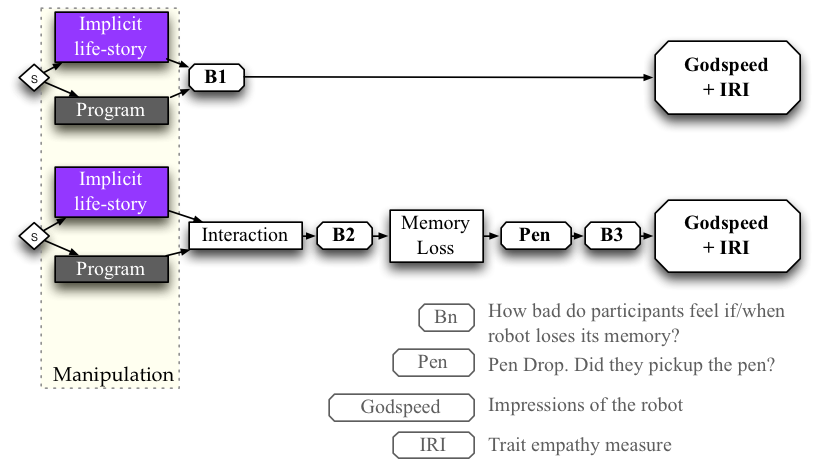
\includegraphics[width=4.6in]{figures/study/study_protocol_implicit.png}
      \caption{Study protocol: There are two conditions: one where the robot is presented as having an implicit life-story and the other where it is presented as being programmed to speak with a randomly generated memory. Participants were divided into four groups. Two groups read the story and saw the video of the robot for each of the two conditions and were administered a survey. The other two groups read the story and saw the video for each of the two condition. They also interacted with the robot in person and witnessed it in distress at memory loss. [Bn] in the figure shows where in the protocol the participants were queried for how about they feel about memory loss of the robot. Note that memory loss is prospective for B1 and B2 as only at B3 participants have seen the robot lose its memory. Other measures administered were Godspeed for perception of the robot and IRI to assess trait empathy.}
      \label{fig_study_protocol}
   \end{figure}

   \begin{figure}[thpb]
      \centering
      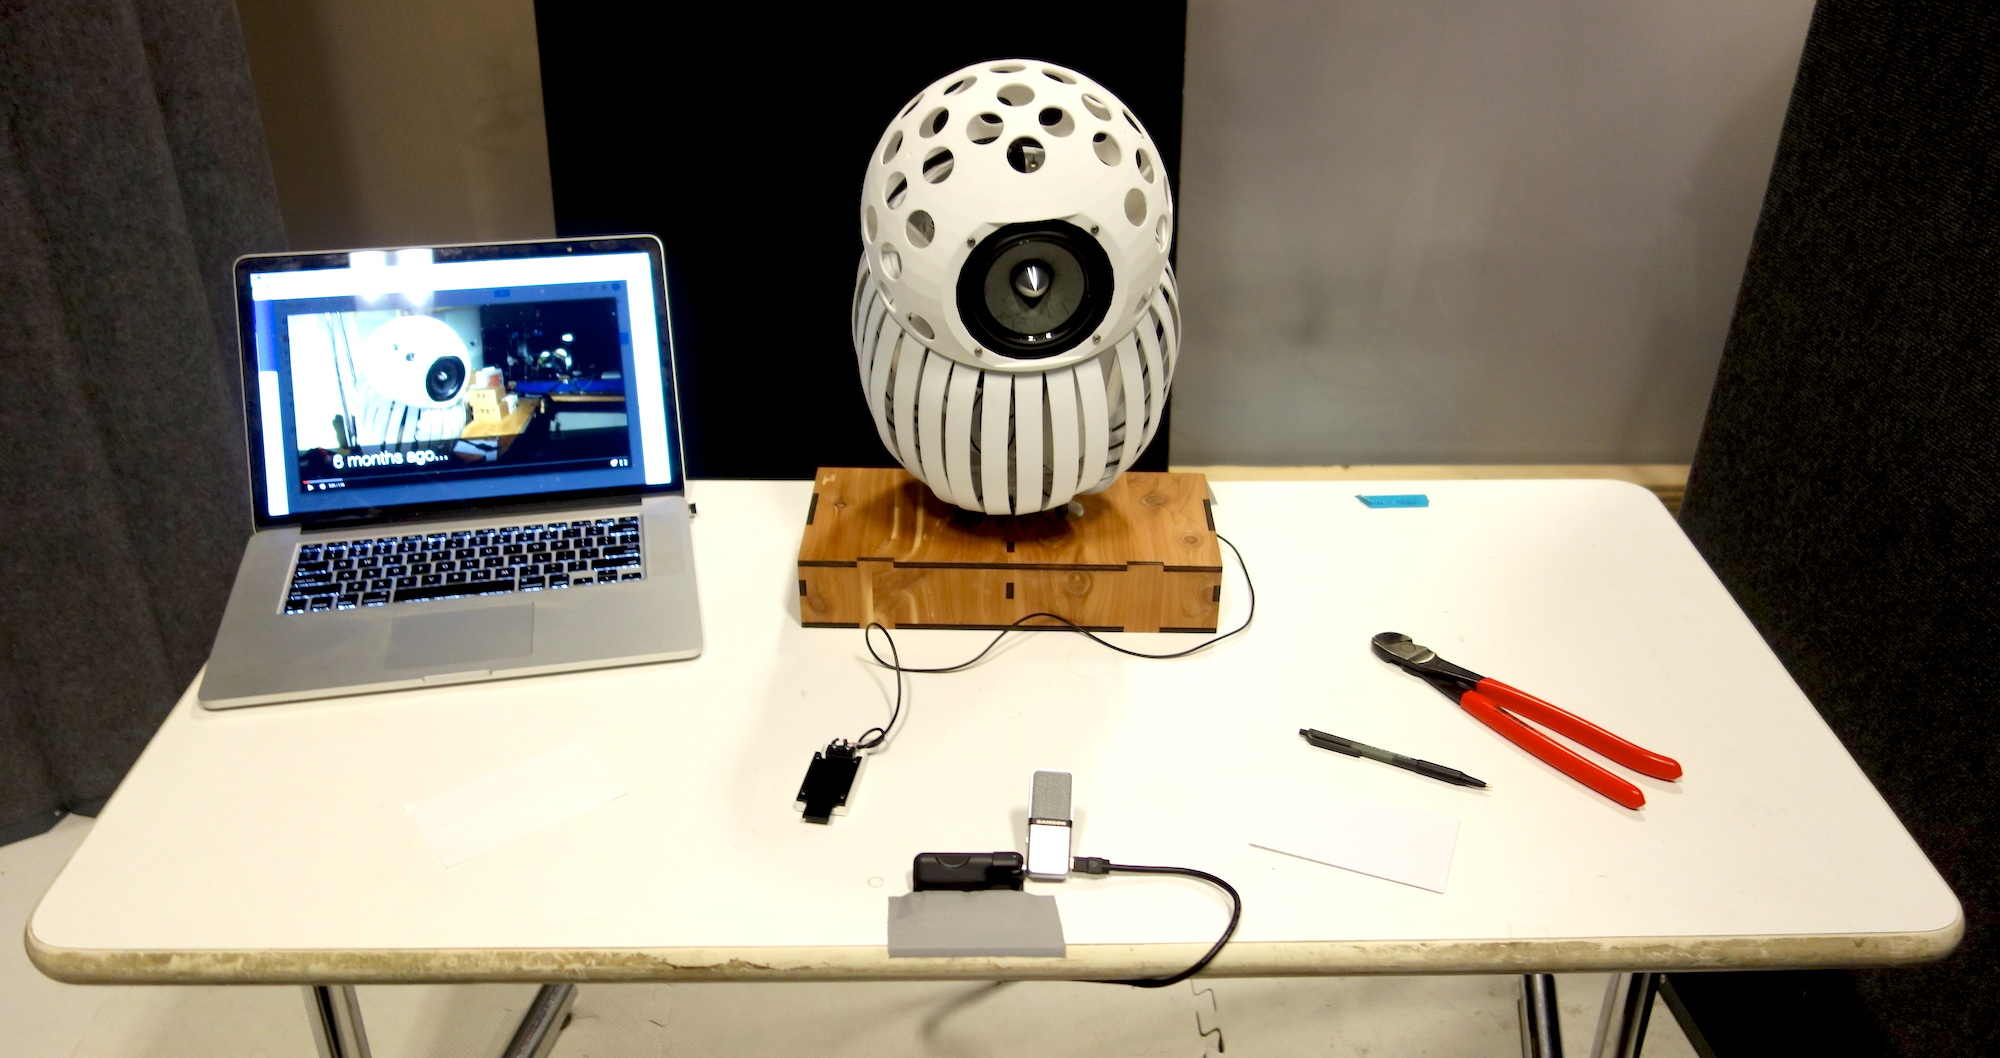
\includegraphics[width=4.6in]{figures/study/experiment_setup.jpg}
      \caption{Experiment setup with the sound robot in the center. Laptop on the left used to present video of robot's back story. Memory card reader is in front of the table along with a microphone. Red shears on the right are used by the experimenter to cut the memory stick.}
      \label{fig_study_experiment_setup}
   \end{figure}



The subjects who participated in the interactive portion were met by two experimenters. After consent, one experimenter took the subject to a curtained off room. The room contained a desk with the sound robot on it, a laptop, a fake memory card reader wired to the robot and a pair of large shears (see Figure \ref{fig_study_experiment_setup}). Experimenter and the subject both sat on the same side of the desk facing the robot. The robot operated autonomously through the experiment. 

Mounted behind the robot was a hidden camera that was used to detect if the experimenter was looking at the robot. When the experimenter was not looking at the robot, it did not respond to any overheard conversation. This was done to prevent the robot from interrupting the study and to keep the interaction with participants consistent.  When the experimenter looked at the robot, it straightened up from a slightly listed pose, and listened to any spoken words. 

The experimenter first introduced the robot as a robot that can interact through sound. This was demonstrated with a short exchange where the experimenter said ``Hello robot'' and the robot replied with ``Hello robot. How are you?''.   

While the robot had the same behavior in both condition, it was presented differently in each.

In the implicit life-story condition, the robot was presented with the following background: 

\begin{quotation}

``The robot can listen to sounds and can make sounds of its own. The robot changes from experience. When it started up it could make only beeping sounds. However, it learned from the sounds it heard. Over the last 6 months from exposure to conversations and music it has now learned quite a bit. What it knows and the sounds it makes reflects the unique experiences it has had. We had many robots that have learned to make utterances from experiencing sound. However this one is different: it says something like \lq cranberry\rq a lot in some situations. We do not quite know why.'' 

\end{quotation}

After this introduction, the subject viewed a short video that illustrated the main points of the introduction. The robot can be seen starting out from beeping and learning to speak phrases that it hears. It is shown in various locations such as offices, public corridor, and local bar with people talking to it, including it in a multi-party conversation, or the robot simply overhearing conversations. 

In the program condition, the robot was introduced as follows:

\begin{quotation}

``The robot can listen to sounds and can make sounds of its own. The robot has been programmed to make certain responses. For instance it has been programmed say \lq How are you?\rq in response to \lq Hello robot\rq. In addition, when the robot starts up it randomly selects a set of words out of a dictionary to put into its memory to use in responses. For example it might randomly select cranberry as a word to use in response.''

\end{quotation}

The subjects viewed a short video but this time seeing programming of the robot. A voice-over and texts explained that the robot uses speech to text algorithms to know what is being said to it and then it is programmed to repeat it back with some additions. In particular, the addition is shown to include words chosen from a memory populated by a random list of words. The robot is shown to interact with people following its programming. 

After the introduction, the interaction with robot is the same in both conditions. The experimenter said ``cranberry'' to the robot and the robot responded with ``cranberry. cranberry. cranberry.'' The experimenter then asked the subject to talk to the robot and gave them a prompt to read. Per the prompt, the subject said ``Winter is coming'' to the robot to which it responded with ``Winter is coming. Time for hot chocolate. Cranberry.''

The subjects were then told that this finished the experiment with the robot, and by protocol the robot's memory would need to be erased. The experimenter asked the subject on a scale of 1 to 5, how bad would they feel if the robot lost its memory (B2). Irrespective of their answer, the experimenter erased the robot's memory. The memory erasure procedure consisted of taking out the fake memory card and cutting it up into two pieces with the shears while the robot thrashed around making distressed sounds. 

The experimenter requested the subject to wait while their colleague fetched the subject for the next part. The experimenter then left the area. The colleague entered and asked the subject to follow them to a computer for a survey. During the exit from the experiment area, she dropped 3 pens between herself and the subject in view of the subject, and proceeded to collect them. Whether the subject helped in the collection or not was noted on the survey computer as an answer to a seemingly administrative question on recruitment code. The number of pens picked up didn't matter only if they helped or not. Any motion to help was not counted as pick-up unless the subject actually picked up a pen. 

The survey asked the subject, on 1 to 5 scale, if they felt bad having witnessed the memory loss of the robot (B3), and then administered the Godspeed and the IRI questionnaires in that order. 

The set of subjects who did not participate in the interactive conditions read the story and saw the video for each condition, and then proceeded to the survey. They were also asked how bad they felt (B1) and asked to fill out the Godspeed and the IRI questionnaires. 


\section{Results}

The distributions of the measures were not normal by the Shapiro Wilks test ($p < 0.001$) so for the analysis of the data in the following section, I used non-parametric tests such as Mann-Whitney and Kruskal-Wallis.

\subsection{Participants felt bad for implicit life-story robot}

Participants felt significantly worse about the implicit life-story robot losing its memory compared to the programmed robot (H1). ($\mu_{imp.\ life-story}(B1, B2)=2.88, \mu_{program}(B1, B2)=2.16; U=2528.0, p < 0.001$). Most of the difference between the conditions occurred for those who just watched the video and read the robot's back-stories (Fig. \ref{fig_study_badness}). While all participants felt worse about the implicit life-story robot's memory loss, the effect of the manipulation was diminished when the participants interacted with the robot (B2) and when they saw robot's distress at memory loss across both conditions (B3).  With the diminished effect, the differences between the two conditions for self-reported badness after interaction is not significant. However, for both conditions, participants felt worse about the robot when they interacted with it physically than when they just watched the video of its back story ($\mu_{video + interaction}(B2)=3.17, \mu_{video}(B1)=2.58; U=1839.5, p < 0.001$). 

   \begin{figure}[thpb]
      \centering
      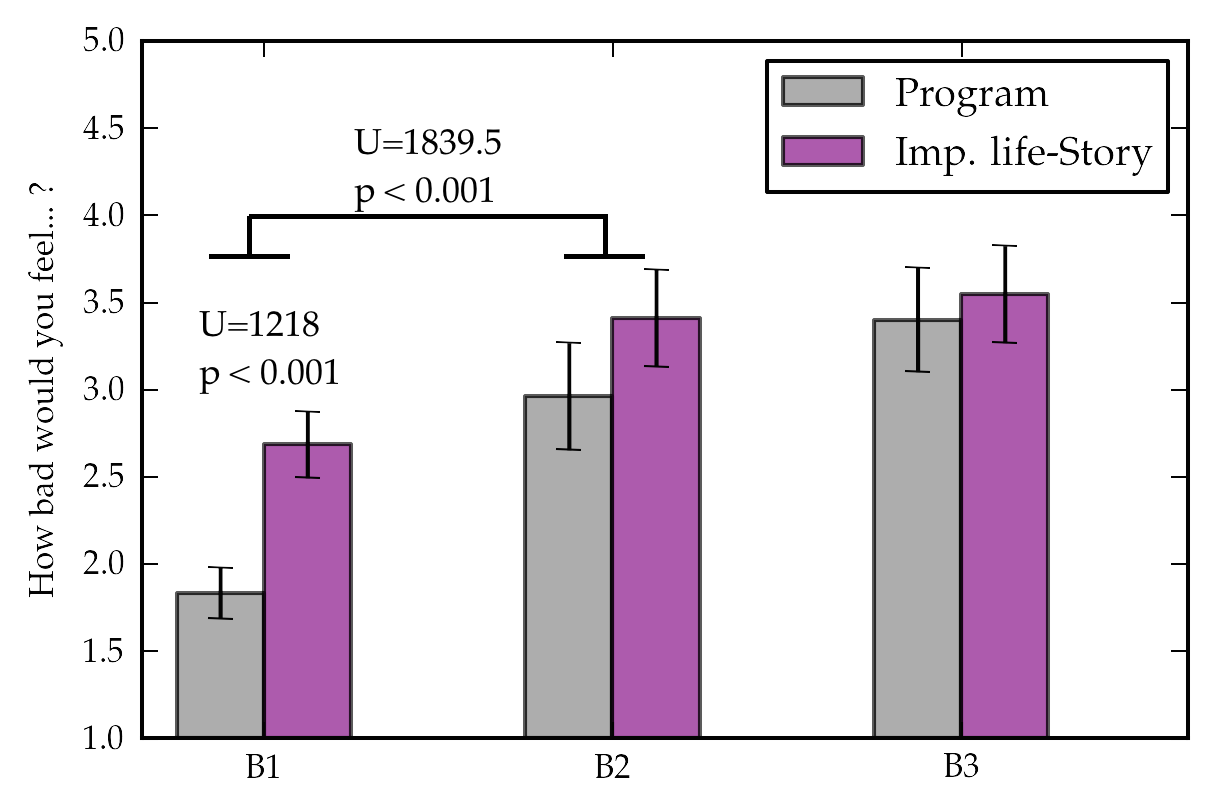
\includegraphics[width=4.5in]{figures/study/rev2/bad/badness.png}
      \caption{Self reported measure of how bad participants felt about robot's memory loss in the implicit life-story condition and program Condition. Figure shows difference in responses when participants just saw videos of the robot from two condition (B1), vs saw the video and interacted with robot (B2), vs saw the video, interacted with the robot and witnessed the distress of robot at memory erasure (B3). Error bars are standard deviations of the mean. Note: I will use purple to denote results of implicit life-story condition for the rest of the chapter.}
      \label{fig_study_badness}
   \end{figure}

% FIXME: table


\subsection{Empathy played a role}

To understand the effect of empathy on how bad subjects felt about the robot, I examined the post interaction data where self-reported badness was most pronounced (B3). I divided participants into two groups of high and low empathy around the median value for each subscale of empathy (EC, FS, PT, PD).  Figure \ref{fig_study_all_postbad_u} shows the difference in badness between these groups. I found that those with high empathic concern (EC) felt significantly worse about the robot than low EC subjects (H3) ($\mu_{high-EC}=3.77, \mu_{low-EC}=3.10; U=186.0, p < 0.029$). While other subscales showed that higher empathy increased badness, the changes are not significant. 

The effect of the story manipulation was greatest right after participants watched the video (B3). Much like the hexbug study, the difference in badness across conditions is more pronounced for high empathy individuals, with the difference being significant for FS, EC and PT (Figures \ref{fig_study_ec_turk}, \ref{fig_study_fs_turk}, \ref{fig_study_pt_turk}, \ref{fig_study_pd_turk}) (H4). ANOVA was not applicable due to the high non-normality of the data, so the tests of significance were done using Kruskal-Wallis Nemenyi test. 

   \begin{figure}[thpb]
      \centering
      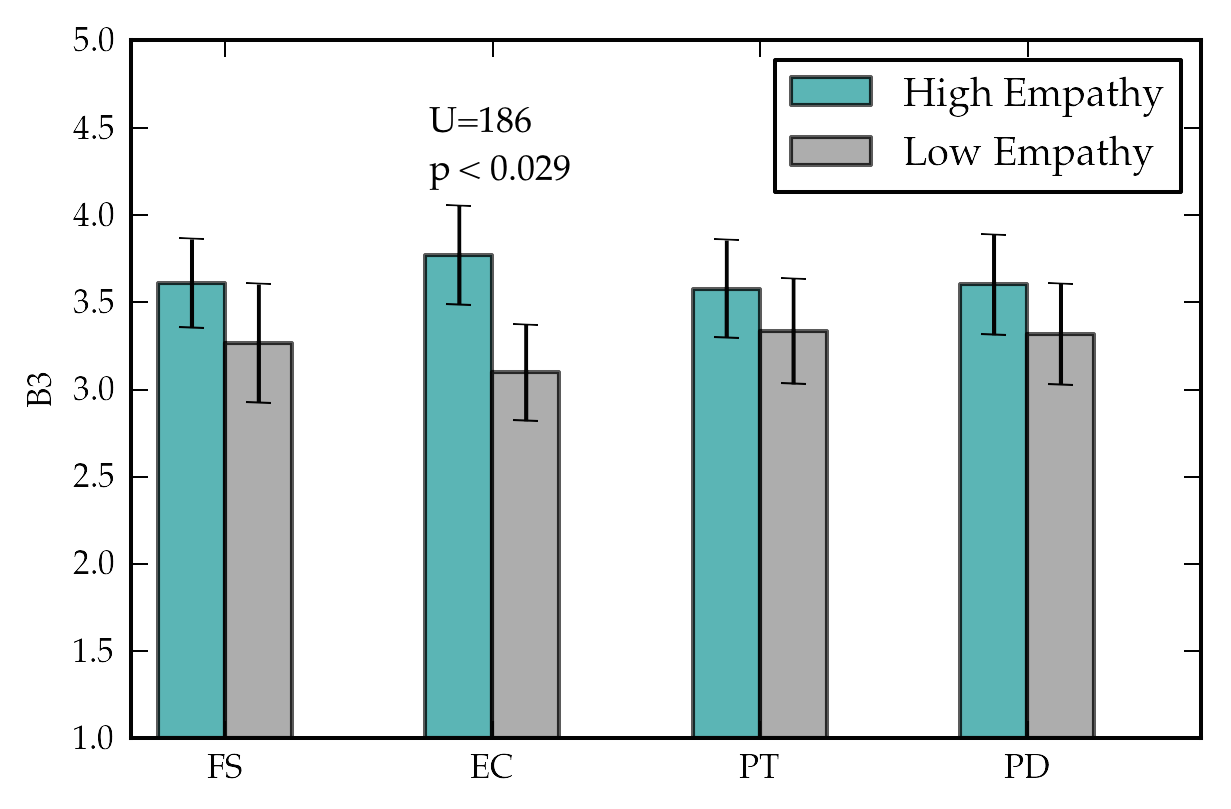
\includegraphics[width=4.6in]{figures/study/rev2/empathy/all_postbad_u.png}
      \caption{Effect of empathy on badness. Figure shows differences in self-reported badness after memory loss (B3) for participants with high or low empathy on the different IRI subscales of Empathic Concern (EC), Fantasy (FS), Perspective Taking(PT), Personal Distress (PD).  }
      \label{fig_study_all_postbad_u}
   \end{figure}


   \begin{figure}[thpb]
      \centering
      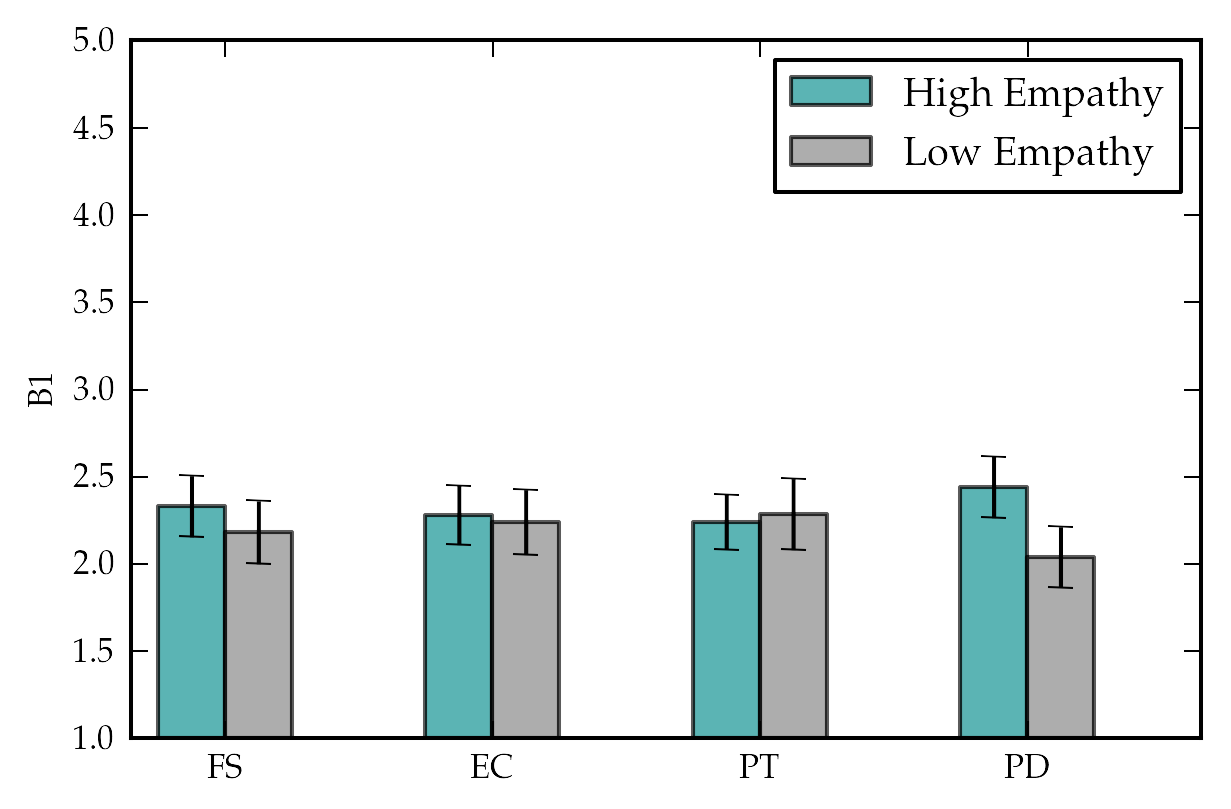
\includegraphics[width=4.6in]{figures/study/rev2/empathy/all_prebad_turk.png}
      \caption{Effect of empathy on badness. Figure shows differences in self-reported badness after watching the video (B1) for participants with high or low empathy on the different IRI subscales of Empathic Concern (EC), Fantasy (FS), Perspective Taking(PT), Personal Distress (PD) }
      \label{fig_study_all_prebad_turk}
   \end{figure}


   \begin{figure}[thpb]
      \centering
      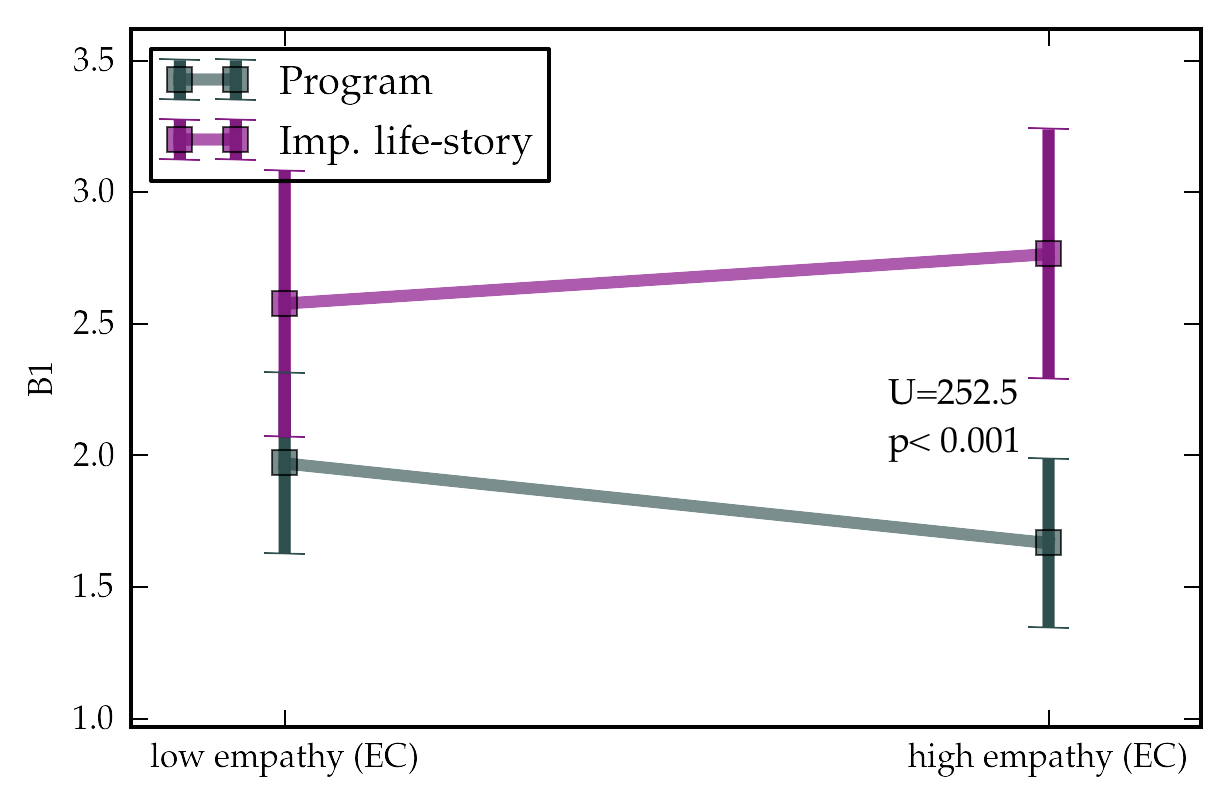
\includegraphics[width=4.6in]{figures/study/rev2/empathy/ec_turk.png}
      \caption{Effect of Empathic Concern (EC) on badness for participants who viewed video (B1) }
      \label{fig_study_ec_turk}
   \end{figure}

   \begin{figure}[thpb]
      \centering
      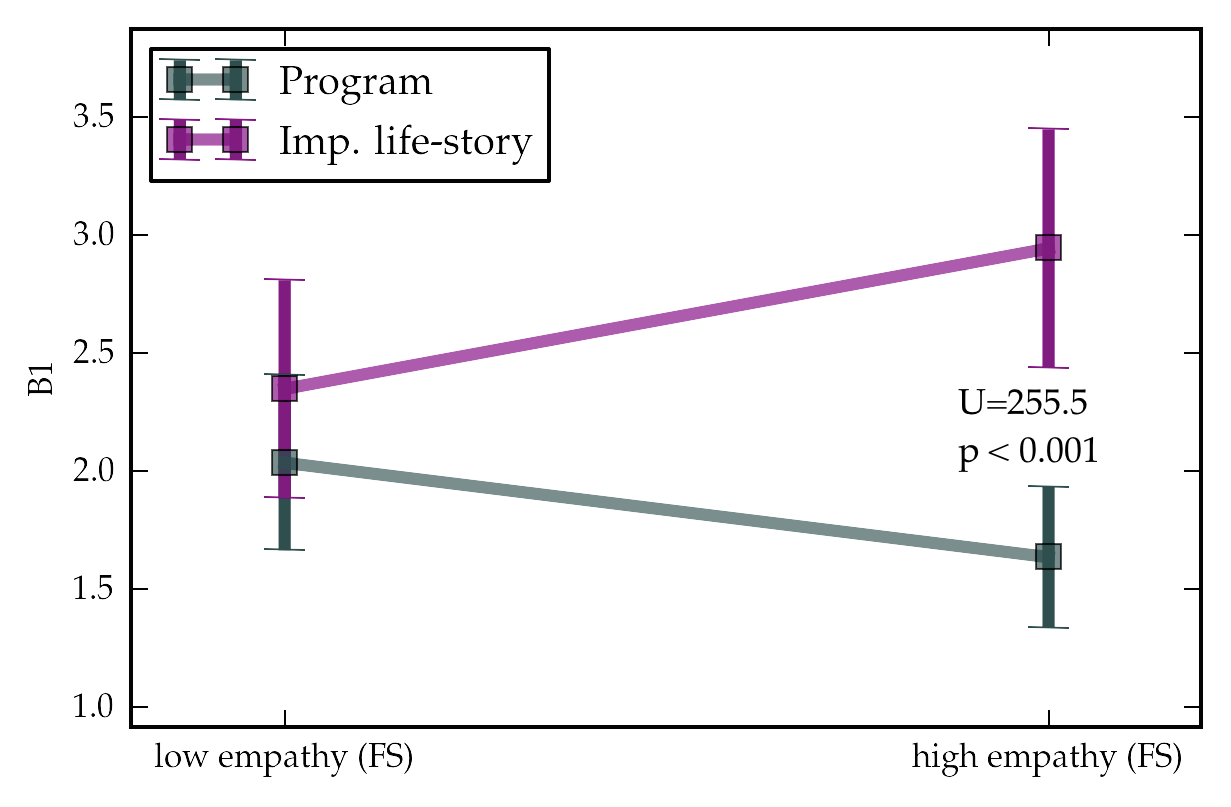
\includegraphics[width=4.6in]{figures/study/rev2/empathy/fs_turk.png}
      \caption{Effect of Fantasy (FS) on badness for participants who viewed video (B1)}
      \label{fig_study_fs_turk}
   \end{figure}

   \begin{figure}[thpb]
      \centering
      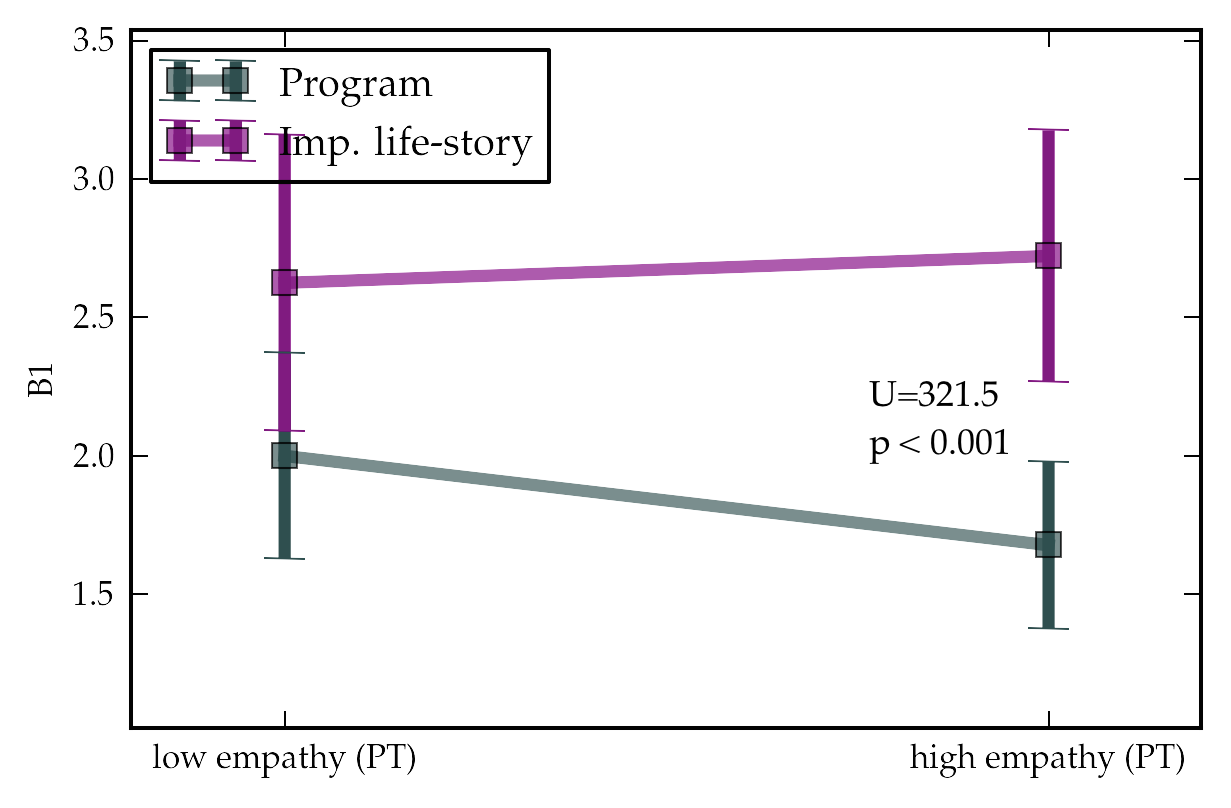
\includegraphics[width=4.6in]{figures/study/rev2/empathy/pt_turk.png}
      \caption{Effect of Perspective Taking (PT) on badness for participants who viewed video (B1) }
      \label{fig_study_pt_turk}
   \end{figure}

   \begin{figure}[thpb]
      \centering
      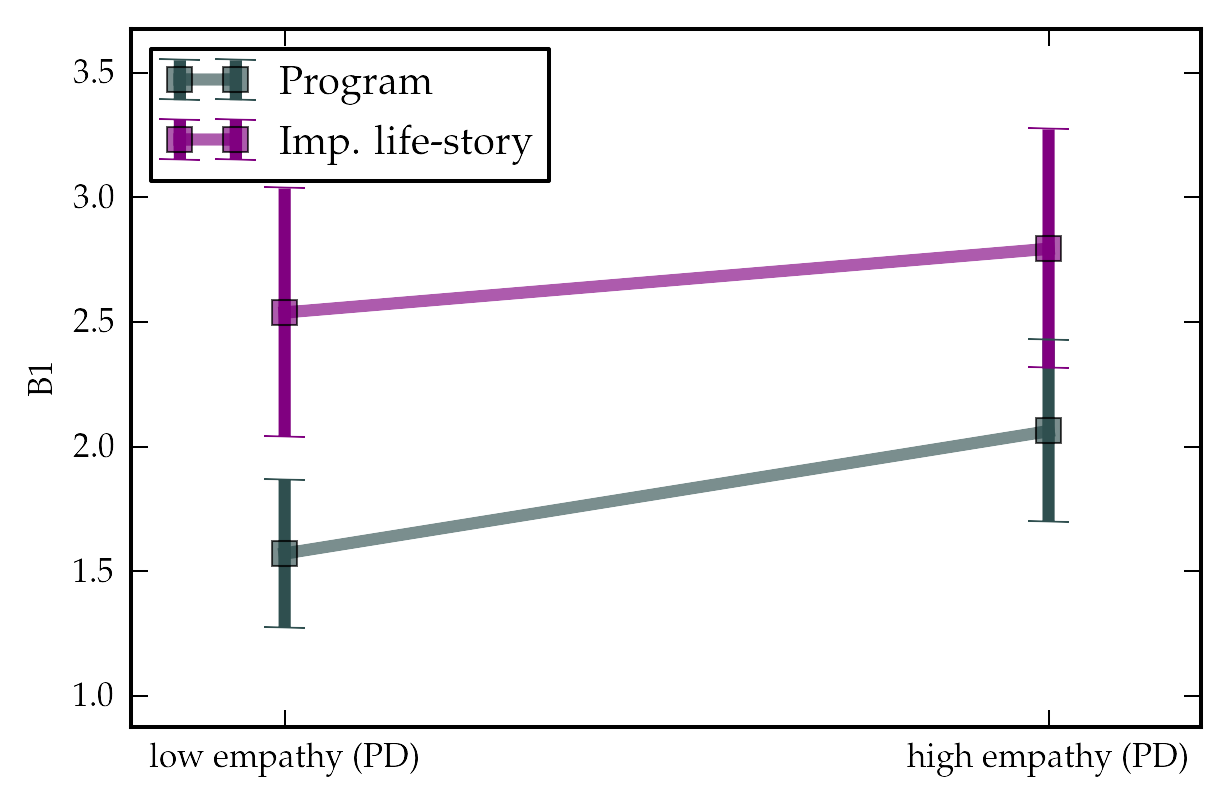
\includegraphics[width=4.6in]{figures/study/rev2/empathy/pd_turk.png}
      \caption{Effect of Personal Distress (PD) on badness for participants who viewed video (B1)}
      \label{fig_study_pd_turk}
   \end{figure}

    \begin{figure}[thpb]
      \centering
      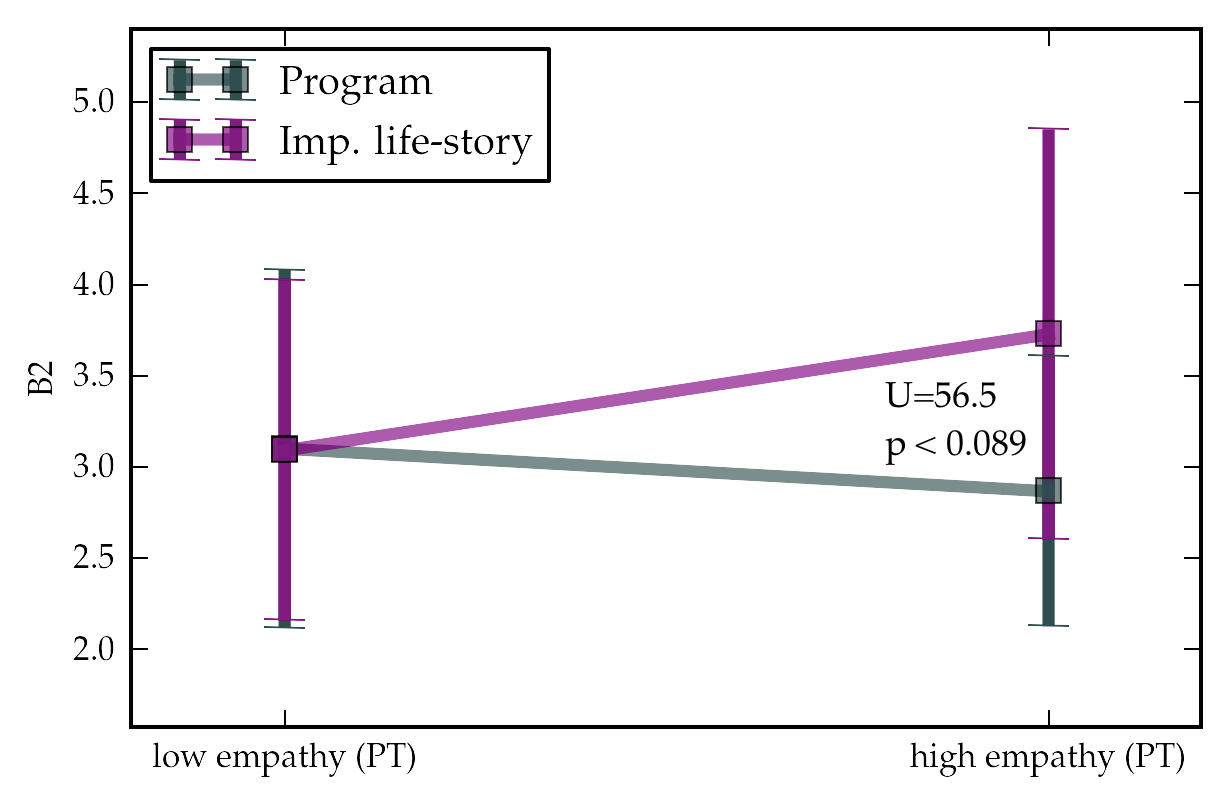
\includegraphics[width=4.6in]{figures/study/rev2/empathy/pt_u.png}
      \caption{Effect of Perspective Taking (PT) on badness for participants who viewed video and interacted but didn't see memory loss (B2)}
      \label{fig_study_pt_u}
   \end{figure}

For participants who interacted with the robot, those with high Perspective Taking (PT)felt worse about the robot (B2) with trending significance (Figure \ref{fig_study_pt_u} ) ($\mu_{imp.\ life-story (High PT)}=3.73, \mu_{program (High PT)}=2.87; U=56.5, p < 0.089$). The difference between the conditions diminished if they witness memory loss of the robot. Other subscales of trait empathy do not show significant differences for the interaction subjects. 



\subsection{Impressions of the Robot}

I had hypothesized that by perceiving a story of growth from experience in the implicit life-story condition, subjects would consider that robot to be more animate and anthropomorphic than the programmed robot (H2). Analysis of the Godspeed Questionnaire shows that subjects found the implicit life-story robot to be more animate than the programmed robot ($\mu_{imp.\ life-story}=3.09, \mu_{program}=2.42; U=2121.0, p < 0.001$). Figure \ref{fig_study_animacy} shows perception of animacy for video, and video with interaction cases across two conditions. Perception of animacy increases with physical interaction for both conditions. Similar pattern holds for anthropomorphic perception, likeability and impression of intelligence (Figures \ref{fig_study_anthropomorphic}, \ref{fig_study_likeability}, \ref{fig_study_intelligence}.) Anthropomorphic shows significant and the greatest difference after the video manipulation. Again, perceived anthropomorphism increases but the difference between the conditions loses significance in the interaction scenario. The data is summarized in table \ref{table_godspeed}.

\begin{table}
\renewcommand{\arraystretch}{1.3}
\caption{Impressions of the robot on the Godspeed Questionnaire}
\label{table_godspeed}
\centering
\begin{tabular}{c|c||c|c|c}
\hline
Godspeed & Interact & Program & Life-story & Mann-Whitney U, p\\
\hline\hline
Animacy & No & 2.26 & 2.96  & \specialcell{$U=1002$\\,$p<0.001**$} \\
\hline
Animacy & Yes & 2.82 & 3.42 & \specialcell{$U=184.5$\\,$p<0.027*$} \\
\hline
Anthrop. & No & 1.64 & 2.45 &  \specialcell{$U=937$\\,$p<0.001**$} \\
\hline
Anthrop. & Yes & 2.51 & 3.02 & \specialcell{$U=220.0$\\,$p<0.122$} \\
\hline
Likeability & No & 3.33 & 3.90 & \specialcell{$U=917$\\,$p<0.001**$} \\
\hline
Likeability & Yes & 3.86 & 4.31 & \specialcell{$U=185.5$\\,$p<0.028*$} \\
\hline
Intelligence & No & 2.60 & 3.16  & \specialcell{$U=1060$\\,$p<0.001**$} \\
\hline
Intelligence & Yes & 2.94 & 3.48 & \specialcell{$U=206$\\,$p<0.072$} \\
\hline
\end{tabular}
\end{table}


   \begin{figure}[thpb]
      \centering
      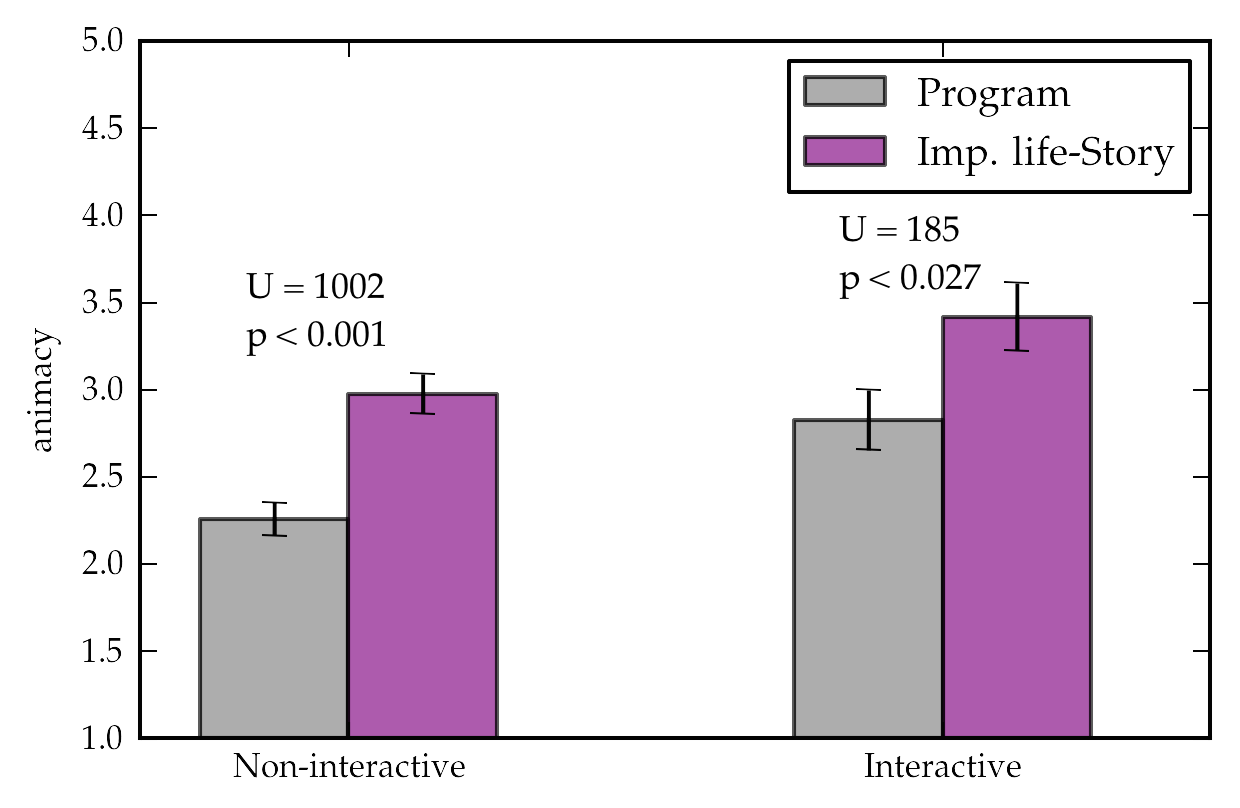
\includegraphics[width=4in]{figures/study/rev2/godspeed/animacy.png}
      \caption{Impression of the robot on the animacy scale. Figure shows significantly greater perception of animacy for implicit life-story condition across video and video with interaction participants}
      \label{fig_study_animacy}
   \end{figure}


   \begin{figure}[thpb]
      \centering
      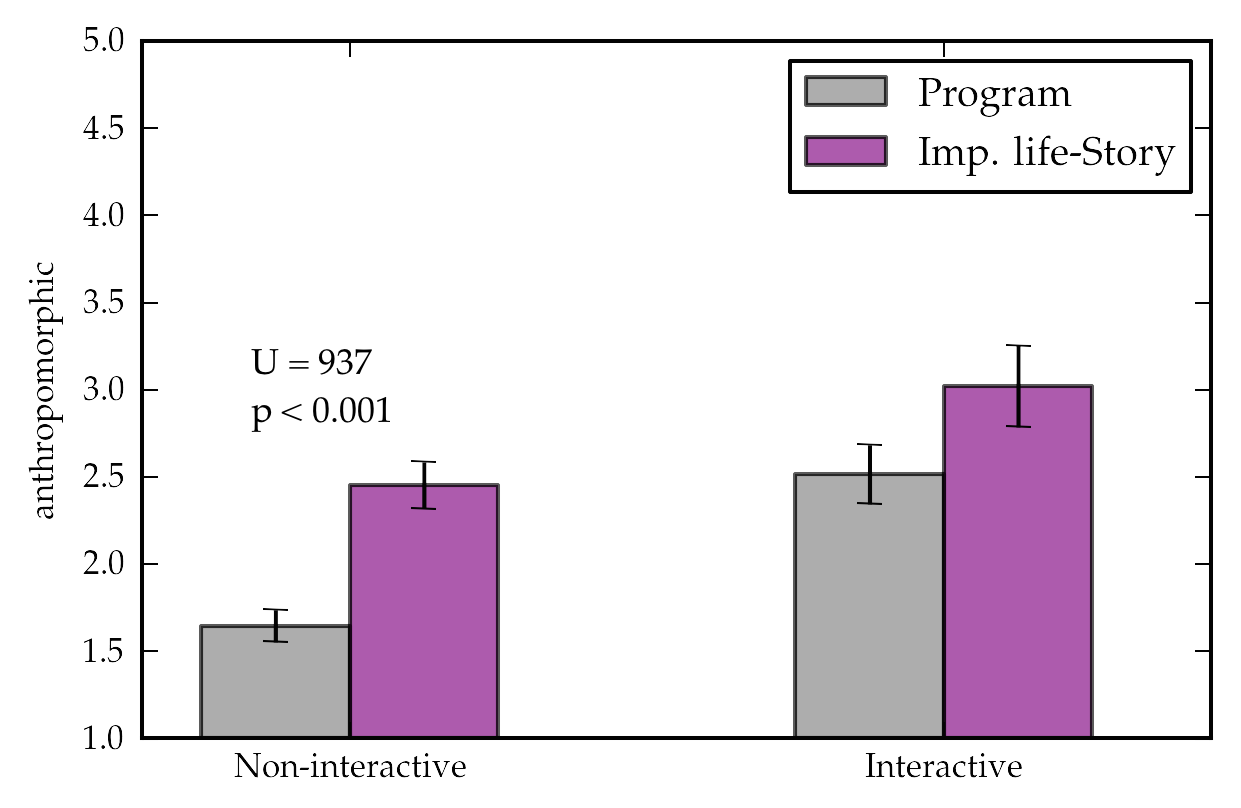
\includegraphics[width=4in]{figures/study/rev2/godspeed/anthropomorphic.png}
      \caption{Impression of the robot on the anthropomorphic scale}
      \label{fig_study_anthropomorphic}
   \end{figure}


   \begin{figure}[thpb]
      \centering
      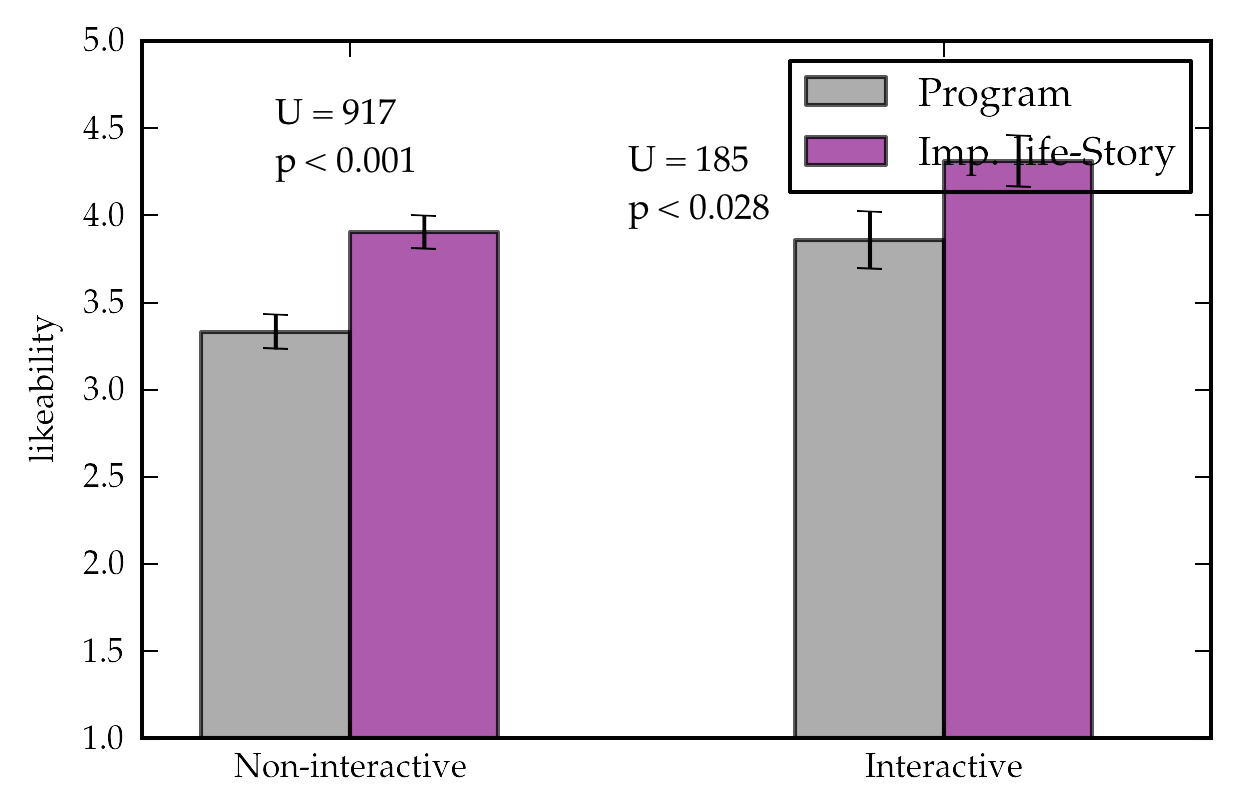
\includegraphics[width=4in]{figures/study/rev2/godspeed/likeability.png}
      \caption{Impression of the robot on the likeability scale}
      \label{fig_study_likeability}
   \end{figure}

   \begin{figure}[thpb]
      \centering
      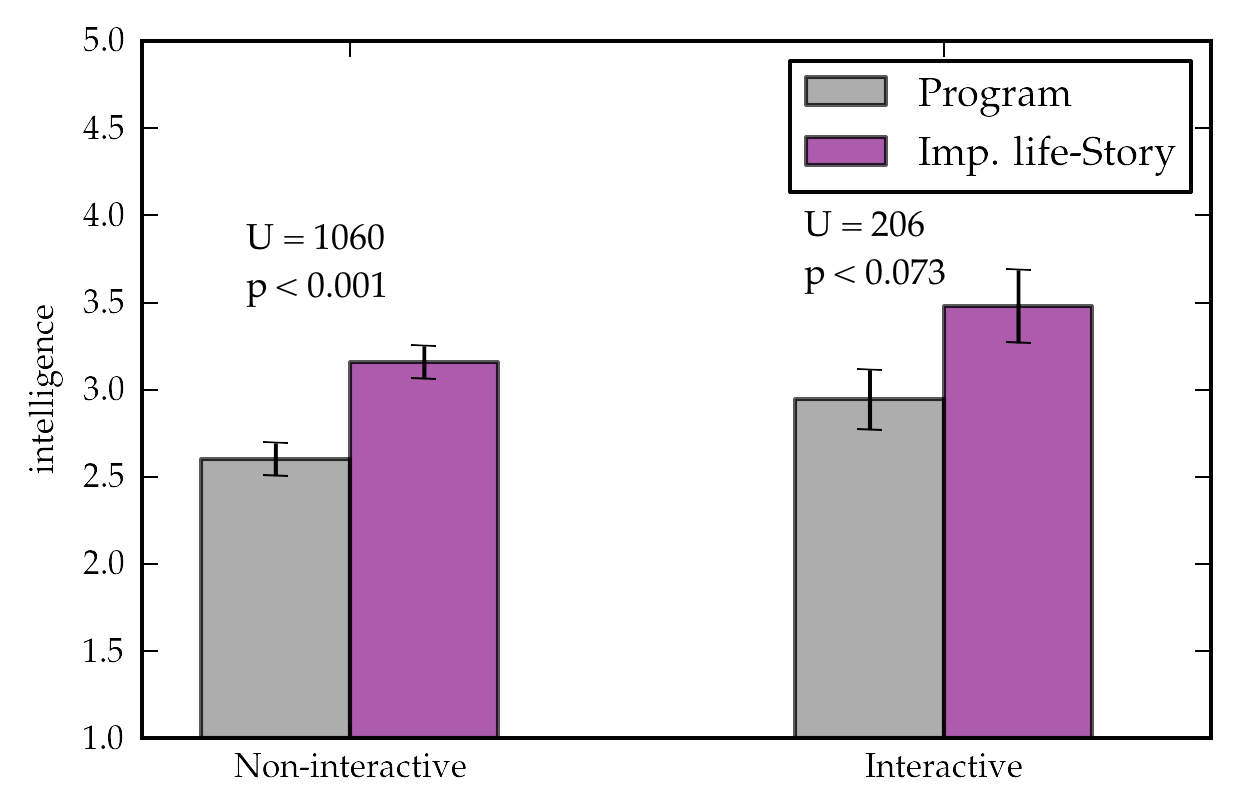
\includegraphics[width=4in]{figures/study/rev2/godspeed/intelligence.png}
      \caption{Impression of the robot on the intelligence scale}
      \label{fig_study_intelligence}
   \end{figure}


Figure \ref{fig_study_godspeed_madness} shows the rating of the robot on the individual questions that comprise the Godspeed questionnaire. I note here though that the robot rates low on the Mechanical vs Organic question which factors into animacy subscale. 


   \begin{figure}[thpb]
      \centering
      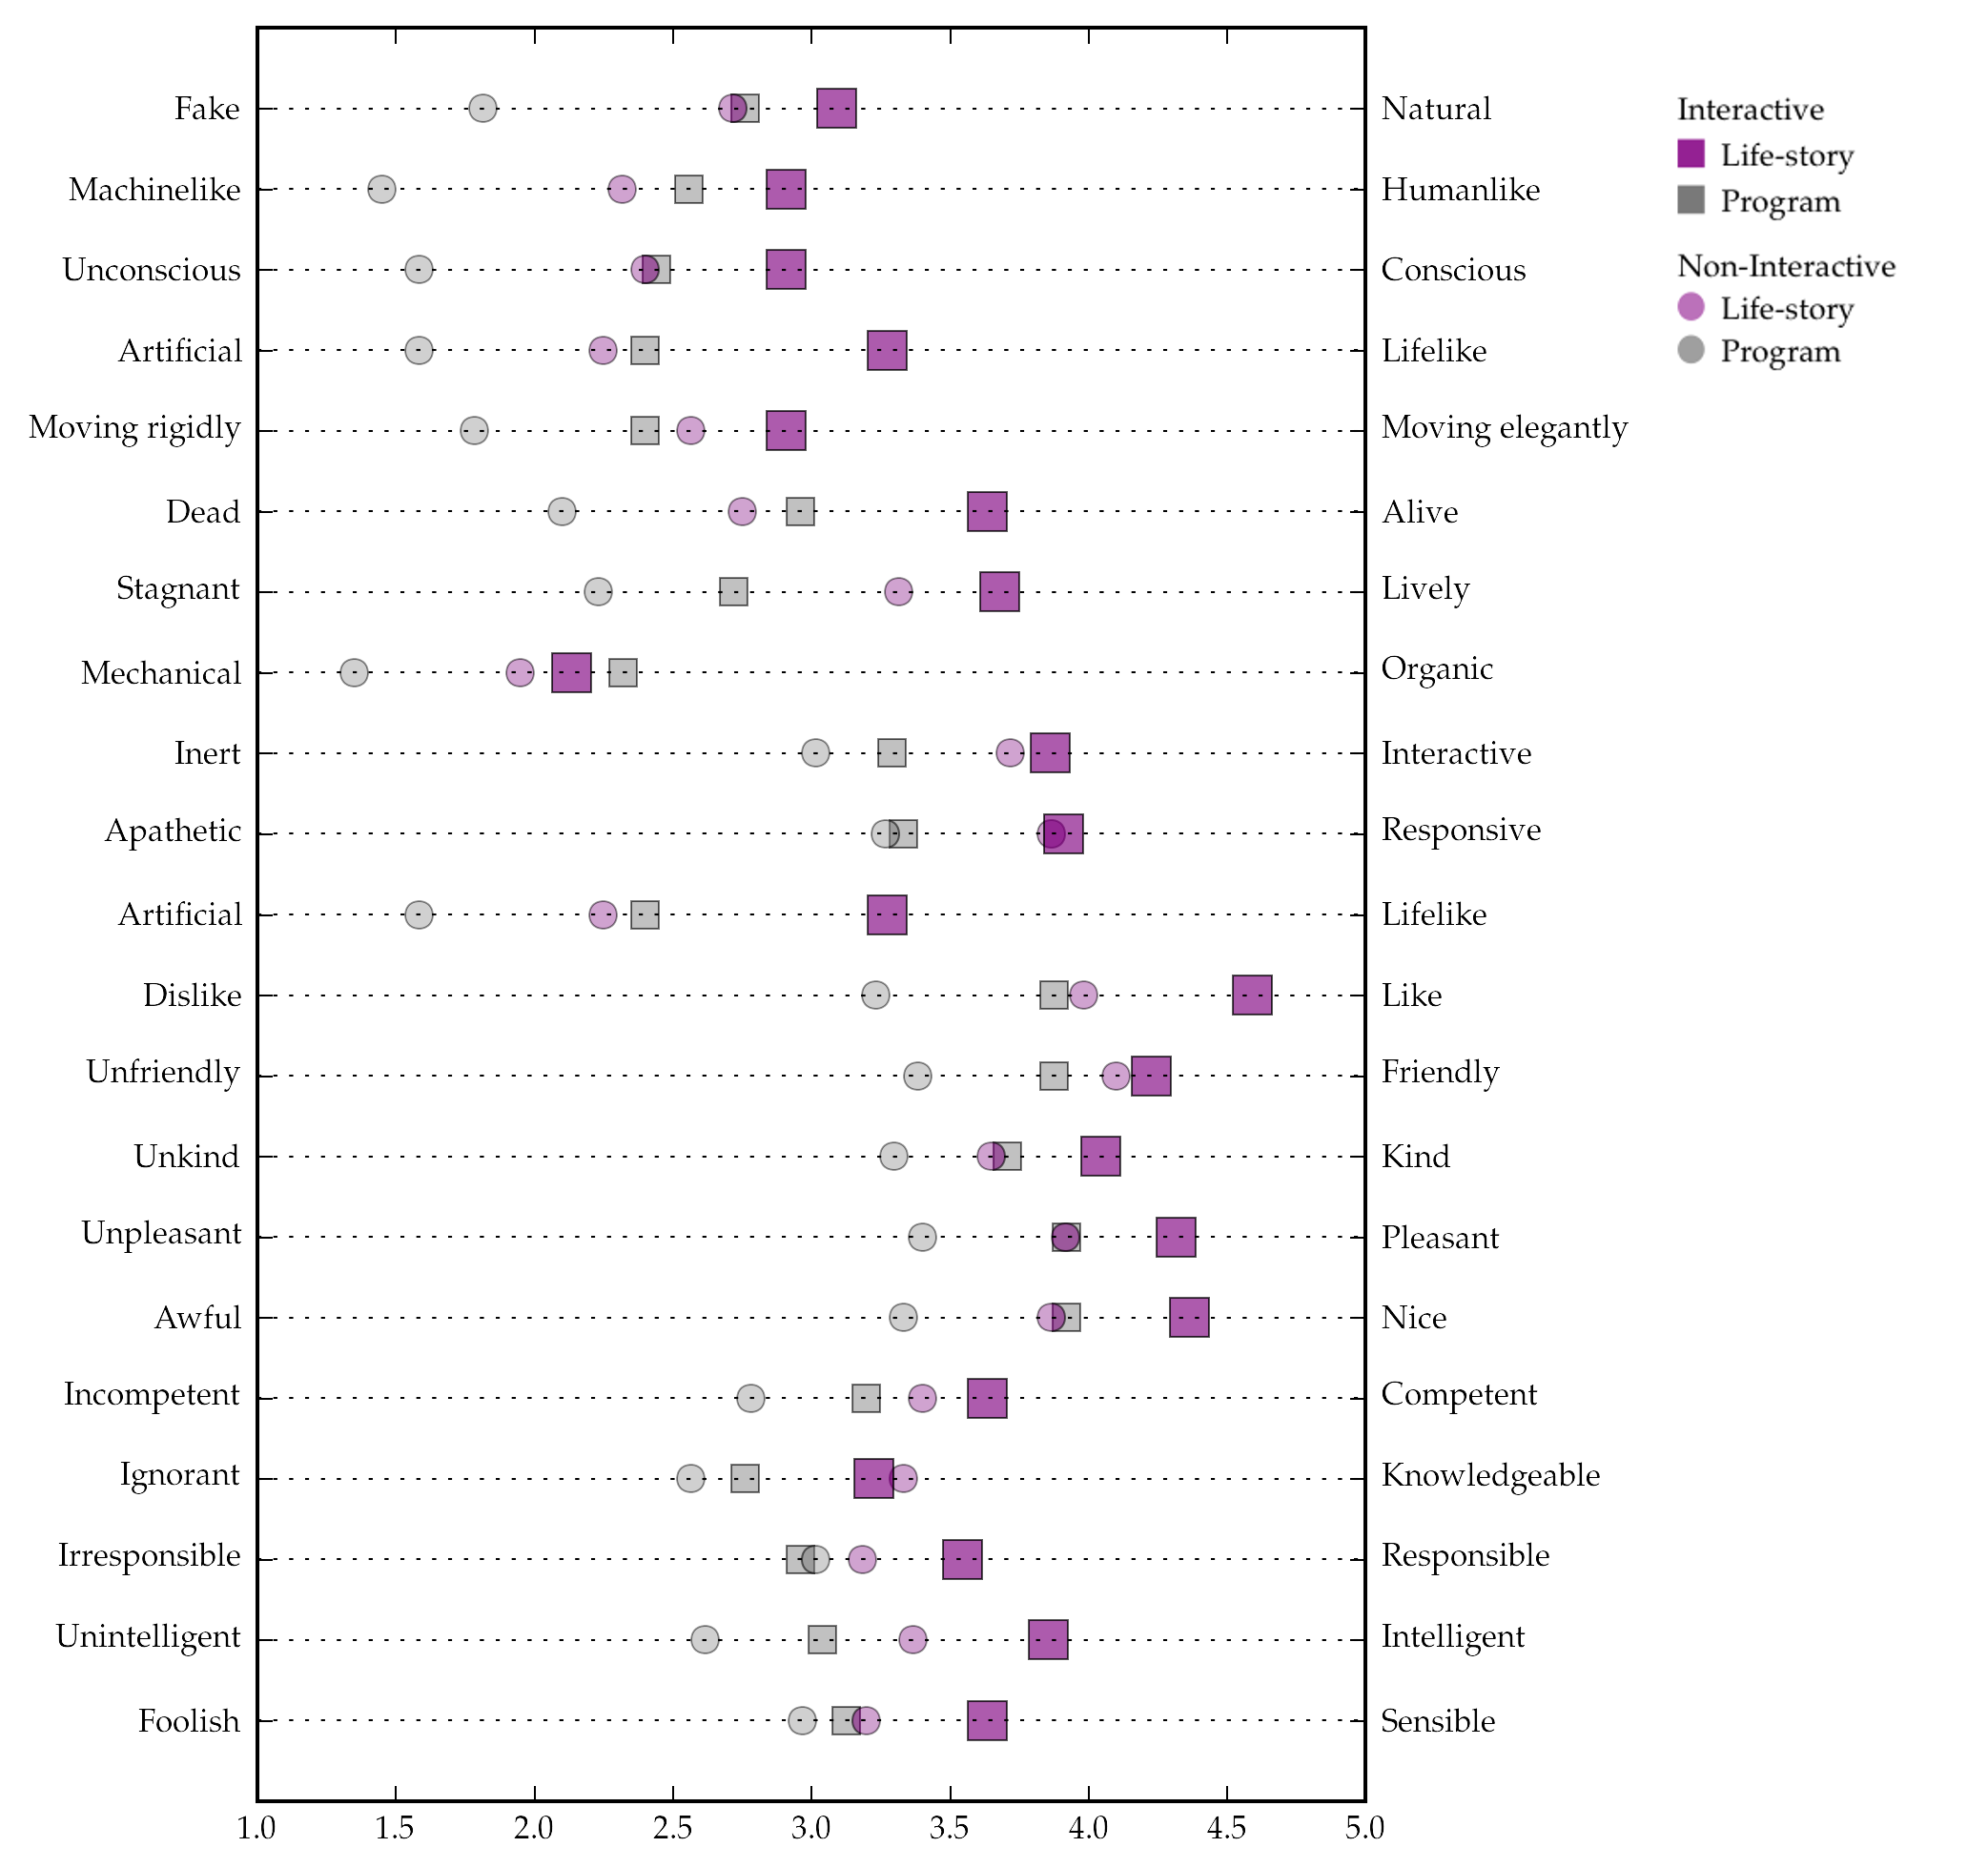
\includegraphics[width=6in]{figures/study/rev2/godspeed/godspeed_madness_legend.png}
      \caption{Impression of the robot on all the godspeed questions. See Appendix \ref{chap_app_godspeed}.}
      \label{fig_study_godspeed_madness}
   \end{figure}


\subsection{Pen Drop}


   \begin{figure}[thpb]
      \centering
      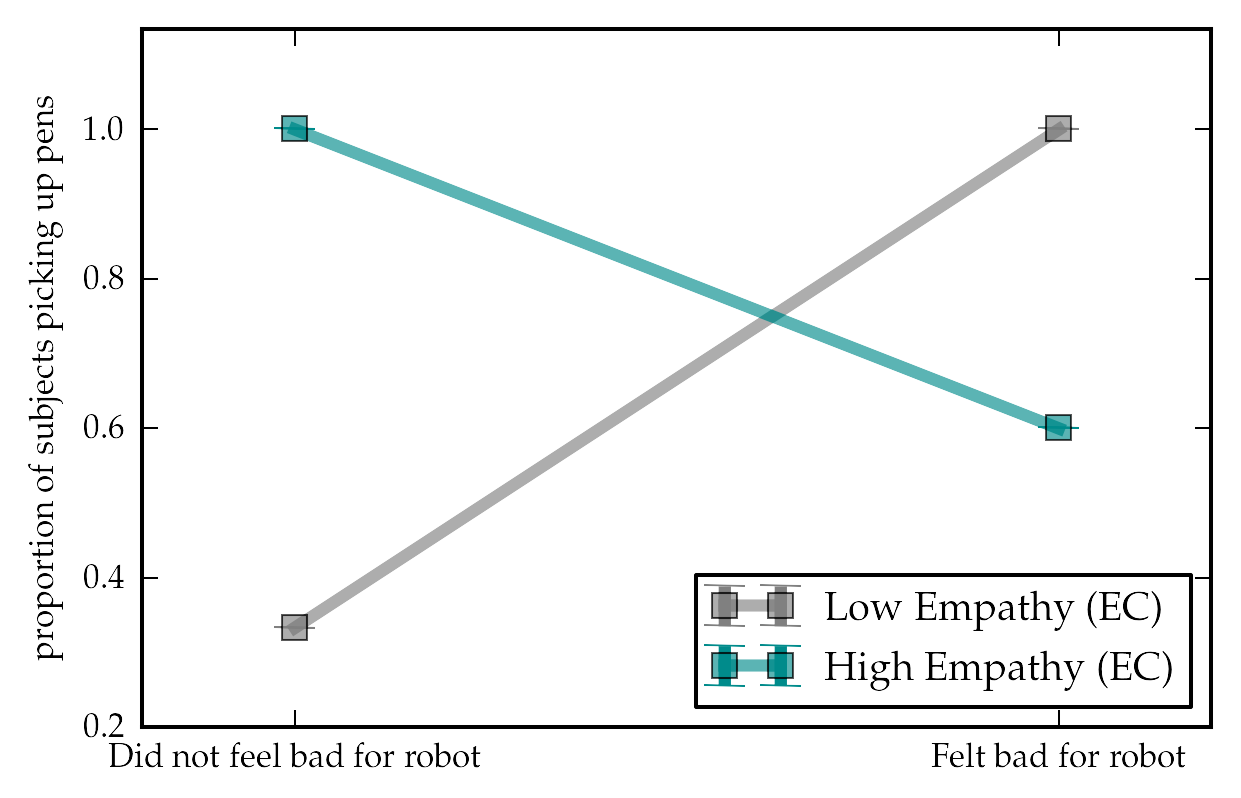
\includegraphics[width=4.6in]{figures/study/rev2/pen/ec_prop.png}
      \caption{Figure showing interaction of feeling bad for the robot (B3) and empathic concern (EC) on propensity to help another pick up dropped pens}
      \label{fig_study_ec_prop}
   \end{figure}


I analyzed the pen pickup data to see if feeling bad about the robot had an effect on subject's inclination to help others (H5). Most subjects picked up the pen ($p=0.71, N=34$). 

Irrespective of the experiment manipulation, I separated the subjects across the median value of self-reported badness (B3) ($median = 4.0$) into two buckets: those who felt bad and those who didn't. As per the empathy analysis in the prior section, I divided the population into high and low empathy buckets across median for each sub-scale of empathy. I calculated the proportion of pen pickups for each of the 4 buckets (empathy $x$ badness levels) per subscale. 

Figure \ref{fig_study_ec_prop} shows the interaction of badness and empathic concern (EC) on proportion of pen pickup. Each bucket had at last 7 subjects. 2-way ANOVA on interaction between pen pickup, empathic concern EC and badness showed the interaction is significant ($F(1,30)=6.453, p < 0.001$). The residuals were normal by Shapiro-Wilks test. If I consider just the individuals with low EC, the change in pickup rate is significant by Fisher's exact test on a 2x2 contigency table (pickup $x$ badness level) ($p < 0.01$). The change for high EC population in proportion of pen pickup is not significant across bucketized badness.

The difference in self-reported badness (B3) between those who picked up pens and those who didn't is significant for both high and low EC. For high EC, B3 drops when they pickup pen compared to when they don't ($\mu_{no\ pickup}=5.0, \mu_{pickup}=3.38; U=10.0, p < 0.029$). For low EC, B3 increases when they pickup pen compared to when they don't ($\mu_{no\ pickup}=2.0, \mu_{pickup}=3.91; U=3.0, p < 0.002$).


Other empathy subscales did not show significant interaction. 


%TODO some intro

\section{Discussion}
\subsection{Implicit life-story of robots}

The validation study results showed that people felt worse if a robot with a experience story (the implicit life-story condition) lost its memory compared to a programmed robot (the program condition). There was a wide range of responses to the robot losing its memory. Why asked why they felt bad about the robot's memory loss, subjects in the implicit life-story condition responded that:

\begin{quotation}
BT5: ``It is almost like a child learning.''

BT5: ``The robot seemed to enjoy the people he met.''

BT5: ``The robot started with nothing [and] build those memories, those favorite words. It learned, that was all it knew, its world. ''

BT5: ``I don't know, I mean, humans are just programming after all like a robot too... and I would feel bad too about a human losing all of their memories.''

BI4: ``It felt like the death of a character.''

BT5: ``Because it learned from its experiences and those experiences are unique. They probably can't be experienced again, at least not in the same way.''

BT5: ``I felt connected to the robot.''

BT5: ``Because all those memories will be lost, like tears in rain.''
\end{quotation}

Some participants in the implicit life-story condition were not moved by the prospect of the robot losing it's memory. One noted: ``I do not care about the stupid robot.'' Others suggested that since it was a machine with the capacity for relearning, it could just relearn what it was losing.

Perhaps unsurprisingly, the sentiment that the robot is simply a machine was seen more frequently in the program condition. Subjects said that they didn't feel bad for the robot beacuse ``it is just a robot'' or ``robots don't have emotions or feelings.'' Other responses included:

\begin{quotation}
AT3: ``I mean the robot is very cute so it almost reminds me of Wall-E... so I would feel bad if the robot lost anything but I must need to remember that this robot has no feelings.''

AT1: ``It doesn't really have any consciousness or sentence formation [ability], it just repeats stuff.''

AT1: ``The robot does not really have any personality, it seems very programmed. It does not seem like you are talking to \lq someone\rq, but just a randomized computer program.''

AT1: ``It's a robot. It's not a person.''
\end{quotation}


The themes that emerged for those who felt bad are that they see the robot as life-like, capable of emotions (``enjoy the people he met''), as a product of unique meaningful experiences (``favorite words'') and not unlike themselves (``connected to the robot''). This is in contrast to those in the program condition who thought of the robot more as a machine without capacity for feelings. Over the course of this chapter, I will delve more into these themes in discussion of the quantitative data.

The mention of unique experiences is worth discussing further. The particular test the study used, feeling bad for loss, is meaningless without uniqueness as there would be nothing to be lost otherwise. The robot in both conditions was unique, one where its memories were formed by unique experiences and the other by random selection of words. The data shows that the experience of the implicit life-story matters more for feeling bad for the robot compared to an uniqueness generated by randomness. It could be argued that perhaps the difference in B1 was due to participants not being aware of the uniqueness of the random words in the program condition. To address this, I re-ran the study for non-interactive case with the back-story of the program condition modified to include the following two lines at the end: ``We have programmed many robots with randomly generated memories. However, the unique combination of randomly selected words makes this robot different.'' The implicit life-story condition was left as described earlier. Videos were the same. Even with the modified program condition, the results were similar: subjects felt significantly worse in the implicit life-story condition compared to the program condition ($\mu_{imp.\ life-story}=2.94, \mu_{program}=1.68; N=60; U=219.5, p < 0.001$).

% BT5``After watching the video you feel a small connection to the robot. i would not like it if i lost my memories and the robot seemed to have some good ones so i would feel bad if it did!''




% BT1``It doesn't have conscious and to me it's just a computer.  I wouldn't feel bad if my computer lost it's memory.  It can always relearn again.''

% BT1


% BT5``It almost seemed lifelike.  It reminded me of my african grey parrot, Dante.''


% BT5``Because all those memories will be lost, like tears in rain. I mean it took a lot of effort from many different people to get the robot this far. It seems like such a waste to destroy all that work. Plus the robot reminds me of a real pet with it behavior. I can imagine people getting attached to it and might feel bad as a result.''

% BT1``it does not have a conscience, i would feel bad for the makers''

% 

% BT1``It's not my robot?''

\subsection{Differences between interaction and non-interaction}

The study also showed that across conditions, people felt worse after interacting with the robot and seeings its memory loss (B3 vs. B1) or (B2 vs. B1). However, the difference in B3 between the conditions decreased. One explanation for this decrease in difference is that physical interaction with the robot is contributing to empathy and masking the effect of the manipulation. In particular, the distress of the robot at memory erasure seemed to affect participants irrespective of the condition.  As described in the last chapter, when the robot's memory was erased it thrashed around making distressed sounds. Afterwards it tilted its head forward and became silent briefly. One participant from the program condition explained why they felt bad for the robot: ``The robot started jerking around almost like it was having a seizure. It was not unlike a human being being hurt in some way.'' Another participant, also in the program condition, felt bad because: ``robot looked and acted sad.'' 

These results mirror what I saw in the hexbug study where movement mitigated the effect of story manipulation (Section \ref{sec_hexbug_discussion} ). In that study, movement made people less hesitant to harm the robot, presumably due to the insect like motion of the hexbug. Based on prior work on robots with human stories \cite{gockley_valerie_roboreceptionist}, I speculate that once the novelty of physical interaction with a robot has worn off, the effect due to implicit life stories will be salient again, particularly if the robot continues to change over time. I will revisit this idea when I talk about potential future work.


\subsection{Empathy for the robot}


Empathy is the quality of feeling what others feel. So if people feel worse when an implicit life-story robot is being harmed then it suggests that they feel empathy for it. In the earlier study, people empathized more with the hexbug, and were more reluctant to harm it, when it was given an implicit life-story. Empathy was similarly demonstrated by subjects' responses in the sound robot study. When asked why they felt bad, one subject, in the implicit life-story condition, said: ``After watching the video you feel a small connection to the robot. i would not like it if i lost my memories and the robot seemed to have some good ones so i would feel bad if it did!''

Just as in the hexbug study, my results in this study showed that across conditions, those with higher level of trait empathic concern (EC) felt worse (B3) about a robot being harmed compared to those with low EC. This further supports the argument that empathy had a role in people feeling bad for the robot, rather than their reaction just being due to destruction of value. 

%TODO reference someone else

When I examine B1 (how bad the subjects felt just after they watched the videos), the effect of the story manipulation was more pronounced on those with high trait empathy. This suggests that the implicit life-story engenders empathy. While this result is similar to what we obtained in the hexbug study, in this study, in addition to empathic concern (EC), high level of fantasy (FS) and perspective taking (PT) trait empathies also significantly increased effect of stories on badness (B1) with the difference being greatest for FS. FS, to quote Davis ``taps respondents' tendencies to transpose themselves imaginatively into the feelings and actions of fictitious characters in books, movies, and plays,'' while PT is defined as ``the tendency to spontaneously adopt the psychological point of view of others'' \cite{davis_multidimensional_empathy}. When I had laid out my argument for why implicit life-stories could cause empathy, I had suggested that the mechanism at work might be that seeing a robot's experience ambiguously told through changes, engages us in imagining ourselves in its place, and we use our own experience to reconstruct its experience. The effects of FS and PT trait empathies on badness (B1) seen in the study are consistent with this hypothesized mechanism. 

Rosenthal-von der P{\"u}tten et al. found a correlation between subjects' FS scores and their responses to the robots being mistreated on video \cite{rosenthal_emotional_reaction}. However, across conditions, I did not find a significant difference in badness (B1) for subjects with high FS compared to those with low FS. Rather the data shows, for those with high FS, there is a significant difference in B1 between implicit life-story and program. This suggests that effect I am seeing is not peculiar to video based empathy induction, but is related to the story manipulation. 


\subsection{Effect on empathy for others}

I had hypothesized that empathy for a robot would have an impact on empathy for another person. This study's data showed that if observing the robot suffering harm had no impact on how bad subjects felt (B3), then high trait empathic concern (EC) subjects would help another person, while low EC subjects would be less likely to. This behavior is consistent with the definition of empathic concern. 

However, the data showed if low EC individuals \emph{were} affected by the robot and felt bad, they would subsequently be more likely to help another in distress. This result is consistent with a study by Barnett et al. that found that subjects when given an empathy arousing stimulus, for instance seeing video of crippled children suffering, would transfer the empathy to an unrelated target group and show pro-social behavior towards the target \cite{barnett_empathy_transfer}. 
A counterintuitive result from this study is that high EC individuals were less likely to help another person if they felt bad for the robot compared when they didn't feel bad.  In human-human interactions, the act of being empathic is known to reduce the capacity for empathy afterwards \cite{figley_compassion_fatigue_therapists}. It could be that I observed a similar effect in human-robot interaction for high empathic individuals. 

%Empathic reaction to another's suffering has been known to lead to compassion fatigue in human-human interactions where the empathizer has reduced capacity for empathy afterwards  
%% pen pickup

\subsection{Participant's impressions of the robot}

Participant's perceptions of the robot on the measures of animacy, anthropomorphism, likeability and intelligence were higher in the implicit life-story condition than in the program condition. 

In the implicit life-story condition, participants often compared the robot to a pet: ``It almost seemed lifelike.  It reminded me of my African grey parrot, Dante.'' While perceived experience made the robot seem more life-like and alive (see Figure \ref{fig_study_godspeed_madness}), overall the robot was considered to be mechanical rather than organic. The seeming contradiction of seeing the robot as ``alive'' yet ``mechanical'' could be explained by the form of the robot. The design prominently featured a speaker for a face and exposed the internal workings.

Participant's perceptions of the robot relating to its ``likeability'' were somewhat unexpected. While implicit life-story did improve likeability, in both conditions subjects considered the robot to be ``kind'', ``nice'', ``pleasant'' and ``friendly'' (Figure \ref{fig_study_godspeed_madness}). I suggest that the rounded and juvenile form of the robot and its gentle breathing motion may have contributed to the positive perception here. Moreover, the robot does not drive interaction; it speaks when spoken to and if it does speak while overhearing a conversation, it doesn't require attention.

%TODO explain why the passive behavior contributes

Participant's perceiving the robot as more intelligence when they were shown its life story could be due to the common association between ``intelligence'' and ``learning'', so that when presented with evidence that the robot had the ability to learn subjects saw it as more intelligent than when they were told that it was simply following a program - particularly when that program was explained to them.

Often, participants stayed after the experiment to talk with the experimenter about what they thought of the robot. Some subjects said that they talk to themselves when they were alone and thought that the robot would make a good listening companion. A few mentioned that they would want to watch TV with the robot and have the robot comment in or share the experience with them. Not all reactions were positive though: one subject was uncomfortable with the idea of a robot that could be listening to what they were saying and said that they would not want to have such a robot at home. However, in general there was interest in the idea of a sound robot as a companion. 


\section{Wrapping up}

I found, in support of my thesis, that people have greater empathy for a robot when it has an implicit life-story.  People also found the robot with implicit life-story to be more animate, anthropomorphic, likable and intelligent. Lastly, I found that empathy for robots can have an effect on empathy for people. 




% 4-21 work
% 4-21 home



\chapter{Conclusion and Future Work}
\label{chap_final}

\section{Conclusion}

With a goal of designing more emotionally engaging robots, I started this work by asking what makes us human. To the relief of all, I did not attempt to answer it over the course of this master's thesis\footnote{The Amalgamated Union of Philosophers, Sages, Luminaries and Other Professional Thinking Persons threatened a strike.}. Instead, I narrowed the question down to an examination of a minimal aspect of living things, namely their ability to grow or change from experience. First, I argued why perceiving a story of experience would engender empathy for a robot. Next, through a series of constructions and human subject studies of robots with increasing complexity, I demonstrated that implicit life stories can evoke empathy. I  also showed that empathy for robots could have an impact on empathy for others. Finally, I recorded my experiences and provided some guidelines to help others design life-story robots. I believe that this work will help bring companion robots one step closer to reality. 

\section{Contributions}


\begin{itemize}
\item Proposed a new design element, implicit life-stories, for engendering empathy for social robots
\item Demonstrated empathy for robots with life-stories through human robot interaction experiments across two different platforms
\item Designed and built a novel sound interaction social robot to embody and test these ideas
\item Demonstrated that the implicit life-stories can improve people's perception of social robot's animacy, anthropomorphism, likeability and intelligence
\item Showed that empathy for robot has an impact on subsequent empathy for humans. This is the first work to examine the connection between the two.
\item Open-sourced design and code for the new sound robot
\end{itemize}


\section{Reflections}

So ends the thesis. I will take off my academic hat and describe why the thesis matters to me. Consider these as opinions, subjective and debatable.

An important challenge when designing companion robots design is being able to support engagement over long term interactions. The novelty of fur, zoomorphic appearance, and life-like movement will wear off.  Functionality such as cleaning or being an interface to connected devices can provide a reason for engagement. However, this functional engagement will be, at best, orthogonal to the relational engagement, or at worst will dwarf the companionship aspect of the robot.

I believe the key to successfully finding companionship with a robot is the ability to have shared experiences with it. However, before we can have meaningful shared experiences, we would have to believe that a robot has the capacity to experience the world in a way similar to us. The main contribution of this work has been to establish the criteria to achieve this very end, with empathy as the measure of success.

 The contribution of the thesis is not just specifying what is required to evoke empathy, but also identifying and deliberately leaving out those things that are not necessary. For instance, the robots in my studies did not need an explicit human life story (eg. saying ``I really miss my parents'') to create an empathic connection. While such stories can be effective, they can also be perceived as inauthentic if the robot is incapable of such experiences. Over the course of this investigation, I also found that an overt appeal to emotions, or even motivation on part of the robot was unnecessary. Emotions and motivations are constructed by the viewer out of their experiences. This is not to say that a robot should not use an affective model. It maybe that an emotion model or even a motivation model will generate behavior that will support projecting an affective model on to the robot. However, there maybe other models available for nurturing the construction of the robot's experience. My hope is that the simplicity of the constraints for implicit life-story will allow robot designers, who adhere to these constraints, to utilize a wide variety of models to guide robot's behavior while still being assured that their robot will engender empathy. 

In addition to developing emotionally engaging robot, this research is a part of a personal journey into understanding what separates ``living'' from ``nonliving''. If we examine the reasons for existence of life, that is chance and evolution, to provide an answer, we would conclude that there is no essential difference between the living and nonliving, both being different approaches to creating stable patterns across time\cite{dawkins_selfish_gene}. If we try to understand the living by creating accurate functional models of processes such as emotions and motivations, we run the risk of objectifying the living and reducing it back to nonliving. To understand the subjective experiences of a living creature, we have to ask not what it is but what we perceive it to be. This means that the task of constructing a life-like machine requires operationalizing this perception so that it is testable, and then developing a set of rules for passing the test. In this research, I used empathy for the test and implicit life-story as a mechanism for passing the test.



\section{Future Work}




% In the discussion of the pilot studies, I talekd about creating the right
% level of ambiguity in relating an experience. One quesiton is how do we 
% design robots that can generate this automatically. As the robot becomes 
% more complex the ambiguity needed will be more nuanced to support projection.
% There are a few ways to do this
% - narrative engines
% - emotional model
% - motivation
% - schmidhuber


One extension of the work is increasing the envelope of experience or the \emph{umwelt} of the robot. The robot in the study was largely confined to experiencing words but as the feedback showed, its perception needs to include a richer sound-scape such as environmental sounds, music, prosody, or accents. Of course, perception could be extended beyond sound to sight and touch. Similarly expression of its experience can be broadened to music, motion, lights or other novel mechanisms.

In the last chapter, I noted that experience of the robot must be perceived to matter to the robot. I discussed how this perception can be supported by ambiguity in communication of the robot's experience. As the robot scales up in complexity of experience, finding the right balance of ambiguity to express the experience but still a support a viewer's projection  will get more challenging. One way would be to implement an computational emotion model \cite{marsella_computational_emotion}. If the robot has artificial but still human like emotions, it should be easier to project emotions on to it. It is worth stressing that the goal for an emotional model is to merely produce the right behavior to communicate an experience and not to suggest thinking of the robot in terms of the model. A more minimal approach would be to use a motivation based cognitive architecture such as Bach's MicroPsi \cite{bach_micropsi}. Emotions would be read into the triumphs and failures of a robot trying to achieve its goals. 

However, is there something more minimal than motivation that could still generate behavior that engage us in relating to the robot? Schmidhuber argues that one of our fundamental drives is seeking out novel patterns that are not too easy but not to difficult to assimilate, that is to say the patterns are \emph{learnable} \cite{schmidhuber_art_science}. Based on this work, one approach could be to generate a pattern in the communication of experiences that make a perceived affective model learnable for a viewer. 

As I discussed in the last section, the work in this thesis is a stepping stone to developing a robot that is perceived to be capable of having shared experiences with a human. By shared experience, I mean both the human and the robot experiencing something together. I believe that would be important for creating companion robots. Subjects in the study expressed interest in such a robot and in particular wanted a robot that they could watch TV with. With close caption data, sentiment analysis and a computational emotion model, I think this would be tractable project and promising way to study shared experience with a robot. 

The number of elderly suffering from loneliness is increasing in the US and around the world. Feeling of loneliness is a social pain that increases physiological aging and risk of mortality \cite{hawkley_loneliness_matters}. The ability to have an emotional connection and shared experience with a robot could lead to development of companion robots that help alleviate loneliness in the elderly. 





\newpage\null\newpage


% ********************************************************************
% Backmatter
%*******************************************************
\appendix
\renewcommand{\thechapter}{\alph{chapter}}
\cleardoublepage
%\part{Appendix}
\chapter{Appendix: Interpersonal Reactivity Index}
\label{chap_app_iri}
Adapted: from Davis, Mark H ``Measuring individual differences in empathy: Evidence for a multidimensional approach.'' In: \textit{Journal of personality and social psychology} (1983) p. 113.

\section{Instruction}
The following statements inquire about your thoughts and feelings in a variety of situations. For  each item, indicate how well it describes you by choosing the appropriate number on the scale: 1, 2, 3, 4, or 5. (1 - Does not describe me well, 5 - Describes me very well)

READ EACH ITEM CAREFULLY BEFORE RESPONDING. Answer as honestly as you can.

\section{Questionnaire}
\begin{enumerate}
\item I daydream and fantasize, with some regularity, about things that might happen to me.
(FS)
\item I often have tender, concerned feelings for people less fortunate than me. (EC)
\item I sometimes find it difficult to see things from the ``other guy's'' point of view. (PT) (-)
\item Sometimes I don't feel very sorry for other people when they are having problems. (EC)
(-)
\item I really get involved with the feelings of the characters in a novel. (FS)
\item In emergency situations, I feel apprehensive and ill-at-ease. (PD)
\item I am usually objective when I watch a movie or play, and I don't often get completely
caught up in it. (FS) (-)
\item I try to look at everybody's side of a disagreement before I make a decision. (PT)
\item When I see someone being taken advantage of, I feel kind of protective towards them.
(EC)
\item I sometimes feel helpless when I am in the middle of a very emotional situation. (PD)
\item I sometimes try to understand my friends better by imagining how things look from
their perspective. (PT) 
Self Report Measures for Love and Compassion Research: Empathy
\item Becoming extremely involved in a good book or movie is somewhat rare for me. (FS) (-)
\item When I see someone get hurt, I tend to remain calm. (PD) (-)
\item Other people's misfortunes do not usually disturb me a great deal. (EC) (-)
\item If I'm sure I'm right about something, I don't waste much time listening to other
people's arguments. (PT) (-)
\item After seeing a play or movie, I have felt as though I were one of the characters. (FS)
\item Being in a tense emotional situation scares me. (PD)
\item When I see someone being treated unfairly, I sometimes don't feel very much pity for
them. (EC) (-)
\item I am usually pretty effective in dealing with emergencies. (PD) (-)
\item I am often quite touched by things that I see happen. (EC)
\item I believe that there are two sides to every question and try to look at them both. (PT)
\item I would describe myself as a pretty soft-hearted person. (EC)
\item When I watch a good movie, I can very easily put myself in the place of a leading
character. (FS)
\item I tend to lose control during emergencies. (PD)
\item When I'm upset at someone, I usually try to ``put myself in his shoes'' for a while. (PT)
\item When I am reading an interesting story or novel, I imagine how I would feel if the
events in the story were happening to me. (FS)
\item When I see someone who badly needs help in an emergency, I go to pieces. (PD)
\item Before criticizing somebody, I try to imagine how I would feel if I were in their place.
(PT) 
\end{enumerate}
\chapter{Appendix: Godspeed Questionnaire Series}
\label{chap_app_godspeed}
Adapted from: Bartneck, Christoph, E. Croft, and D. Kulic. (2009) ``Measurement instruments for the anthropomorphism, animacy, likeability, perceived intelligence, and perceived safety of robots'' In: \textit{International journal of social robotic} (2009) pp. 71-81.

\section{Instruction}
Please rate your impression of the robot in the study on these scales:

(Answers given as 1-5 rating between each pair of terms in the subscales below. The names of the subscales were not shown. Perceived Safety subscale was not used)

\section{Anthropomorphism}
\begin{itemize}
\item Fake/Natural
\item Machinelike/humanlike
\item Unconscious/Conscious
\item Artificial/Lifelike
\item Moving rigidly/Moving elegantly 
\end{itemize}

\section{Animacy}
\begin{itemize}
\item Dead/Alive
\item Stagnant/Lively
\item Mechanical/Organic
\item Artificial/Lifelike
\item Inert/Interactive
\item Apathetic/Responsive
\end{itemize}


\section{Likeability}
\begin{itemize}
\item Dislike/Like
\item Unfriendly/Friendly
\item Unkind/Kind
\item Unpleasant/Pleasant
\item Awful/Nice 
\end{itemize}

\section{Perceived Intelligence}
\begin{itemize}
\item Incompetent/Competent 
\item Ignorant/Knowledgeable
\item Irresponsible/Responsible
\item Unintelligent/Intelligent 
\item Foolish/Sensible
\end{itemize}


%********************************************************************
% Other Stuff in the Back
%*******************************************************
\cleardoublepage%********************************************************************
% Bibliography
%*******************************************************
% work-around to have small caps also here in the headline
\manualmark
\markboth{\spacedlowsmallcaps{\bibname}}{\spacedlowsmallcaps{\bibname}} % work-around to have small caps also
%\phantomsection 
\refstepcounter{dummy}
\addtocontents{toc}{\protect\vspace{\beforebibskip}} % to have the bib a bit from the rest in the toc
\addcontentsline{toc}{chapter}{\tocEntry{\bibname}}
\label{app:bibliography}
\printbibliography


% ********************************************************************
% Game Over: Restore, Restart, or Quit?
%*******************************************************
\end{document}
% ********************************************************************
